% ============================================================================
% Tesis — Actualización del núcleo tecnológico de EDDIE (versión preliminar)
% Este main.tex sirve para compilar y revisar los capítulos. Para la entrega,
% usa la plantilla oficial del Departamento: copia capitulos/, datos/,
% figuras/, referencias.bib y comandos_eddie.tex a tu proyecto de Overleaf y
% sigue las instrucciones de LEEME.md.
% ============================================================================
\documentclass[12pt,letterpaper,oneside]{report}
\usepackage[utf8]{inputenc}
\usepackage[T1]{fontenc}
\usepackage[spanish,es-tabla,es-nodecimaldot,es-noshorthands]{babel}
\usepackage{helvet}
\renewcommand{\familydefault}{\sfdefault}
\usepackage[left=3cm,right=2.5cm,top=3cm,bottom=2.5cm]{geometry}
\usepackage{setspace}
\onehalfspacing
\setlength{\parindent}{2.5em}
\usepackage[labelsep=colon,font=small]{caption}
\captionsetup[table]{position=top}
\usepackage[round,authoryear]{natbib}
\usepackage{titlesec}
\titleformat{\chapter}[hang]{\normalfont\Large\bfseries\raggedright}{CAPÍTULO \thechapter.}{0.5em}{\MakeUppercase}
\titlespacing*{\chapter}{0pt}{0pt}{24pt}
\titleformat{\section}{\normalfont\large\bfseries}{\thesection}{0.6em}{\MakeUppercase}
\titleformat{\subsection}{\normalfont\normalsize\bfseries}{\thesubsection}{0.6em}{}
\titleformat{\subsubsection}{\normalfont\normalsize\itshape}{\thesubsubsection}{0.6em}{}
\setcounter{secnumdepth}{3}
\setcounter{tocdepth}{3}
% ============================================================================
% comandos_eddie.tex — paquetes y comandos que usan los capítulos de la tesis.
% En tu proyecto de Overleaf: agrega % ============================================================================
% comandos_eddie.tex — paquetes y comandos que usan los capítulos de la tesis.
% En tu proyecto de Overleaf: agrega % ============================================================================
% comandos_eddie.tex — paquetes y comandos que usan los capítulos de la tesis.
% En tu proyecto de Overleaf: agrega \input{comandos_eddie} al preámbulo de tu
% plantilla (después de sus propios paquetes). Si la plantilla ya carga alguno
% de estos paquetes no pasa nada: LaTeX no los carga dos veces.
% ============================================================================
\usepackage{graphicx}
\usepackage{booktabs}
\usepackage{tabularx}
\usepackage{longtable}
\usepackage{array}
\usepackage{multirow}
\usepackage{amsmath}
\usepackage{amssymb}
\usepackage[table]{xcolor}
\usepackage{float}
\usepackage{tikz}
\usetikzlibrary{arrows.meta,positioning,fit,backgrounds,shapes.geometric}
\usepackage[ruled,vlined,linesnumbered,spanish,onelanguage]{algorithm2e}
\usepackage{tcolorbox}
\usepackage{xurl}  % \nolinkurl corta nombres de archivo largos en cualquier punto

\definecolor{eddietinta}{HTML}{1B2440}
\definecolor{eddieacento}{HTML}{0B7A87}
\definecolor{eddiepend}{HTML}{B26A00}
\definecolor{eddiefondo}{HTML}{EEF1F6}

% Pie de tablas y figuras: «Fuente: …» (igual que en la plantilla del borrador)
\providecommand{\fuente}[1]{\par\vspace{2pt}{\footnotesize\centering\textit{Fuente:} #1\par}}

% Resultado que todavía no existe (se mide en el laboratorio). Se ve en el PDF para no olvidarlo.
\newcommand{\pendiente}[1]{{\color{eddiepend}\footnotesize\textsf{[Pendiente:} #1\textsf{]}}}

% Etiqueta del tipo de medición de cada prototipo
\newcommand{\tipomed}[1]{\textsf{\footnotesize[#1]}}

% Ficha de validación de un prototipo (misma estructura del borrador)
% #1 título, #2 etiqueta, #3 objetivo, #4 librerías/hardware, #5 contrato, #6 requisitos, #7 resultados
\newcommand{\ficha}[7]{%
\begin{table}[H]
\centering
\caption{Ficha de validación del prototipo: #1.}
\label{#2}
\small
\begin{tabularx}{\textwidth}{>{\bfseries}p{3.2cm} X}
\toprule
Objetivo & #3 \\ \midrule
Librerías / Hardware & #4 \\ \midrule
Contrato destino & #5 \\ \midrule
Requisitos asociados & #6 \\ \midrule
Resultados y hallazgos & #7 \\ \bottomrule
\end{tabularx}
\fuente{Elaboración propia, con \texttt{mediciones/medir\_prototipos.py} (P-00).}
\end{table}}

% Resultados numéricos generados a partir de las evidencias (ver datos/actualizar_datos.py)
\input{datos/prototipos_datos}
\input{datos/avances_datos}

% Figura que está en tu Overleaf pero no en este paquete: si el archivo existe se
% incluye; si no, se dibuja un recuadro con el nombre que debe tener.
\newcommand{\figuraopcional}[2]{%
  \IfFileExists{#1}{\includegraphics[width=#2]{#1}}{%
    \fbox{\parbox[c][4cm][c]{#2}{\centering\footnotesize Subir a Overleaf:\\ \texttt{\detokenize{#1}}}}}}

% Nombres largos de código (con guion bajo) pueden cortarse al final de línea.
\let\eddieunderscore\_
\renewcommand{\_}{\eddieunderscore\allowbreak}
\setlength{\emergencystretch}{3em}
 al preámbulo de tu
% plantilla (después de sus propios paquetes). Si la plantilla ya carga alguno
% de estos paquetes no pasa nada: LaTeX no los carga dos veces.
% ============================================================================
\usepackage{graphicx}
\usepackage{booktabs}
\usepackage{tabularx}
\usepackage{longtable}
\usepackage{array}
\usepackage{multirow}
\usepackage{amsmath}
\usepackage{amssymb}
\usepackage[table]{xcolor}
\usepackage{float}
\usepackage{tikz}
\usetikzlibrary{arrows.meta,positioning,fit,backgrounds,shapes.geometric}
\usepackage[ruled,vlined,linesnumbered,spanish,onelanguage]{algorithm2e}
\usepackage{tcolorbox}
\usepackage{xurl}  % \nolinkurl corta nombres de archivo largos en cualquier punto

\definecolor{eddietinta}{HTML}{1B2440}
\definecolor{eddieacento}{HTML}{0B7A87}
\definecolor{eddiepend}{HTML}{B26A00}
\definecolor{eddiefondo}{HTML}{EEF1F6}

% Pie de tablas y figuras: «Fuente: …» (igual que en la plantilla del borrador)
\providecommand{\fuente}[1]{\par\vspace{2pt}{\footnotesize\centering\textit{Fuente:} #1\par}}

% Resultado que todavía no existe (se mide en el laboratorio). Se ve en el PDF para no olvidarlo.
\newcommand{\pendiente}[1]{{\color{eddiepend}\footnotesize\textsf{[Pendiente:} #1\textsf{]}}}

% Etiqueta del tipo de medición de cada prototipo
\newcommand{\tipomed}[1]{\textsf{\footnotesize[#1]}}

% Ficha de validación de un prototipo (misma estructura del borrador)
% #1 título, #2 etiqueta, #3 objetivo, #4 librerías/hardware, #5 contrato, #6 requisitos, #7 resultados
\newcommand{\ficha}[7]{%
\begin{table}[H]
\centering
\caption{Ficha de validación del prototipo: #1.}
\label{#2}
\small
\begin{tabularx}{\textwidth}{>{\bfseries}p{3.2cm} X}
\toprule
Objetivo & #3 \\ \midrule
Librerías / Hardware & #4 \\ \midrule
Contrato destino & #5 \\ \midrule
Requisitos asociados & #6 \\ \midrule
Resultados y hallazgos & #7 \\ \bottomrule
\end{tabularx}
\fuente{Elaboración propia, con \texttt{mediciones/medir\_prototipos.py} (P-00).}
\end{table}}

% Resultados numéricos generados a partir de las evidencias (ver datos/actualizar_datos.py)
% Generado por mediciones/medir_prototipos.py — no editar a mano; volver a ejecutar el script.
\newcommand{\MedicionFecha}{2026-11-08}
\newcommand{\MedicionSistema}{Linux 6.18.44-fc-v310}
\newcommand{\MedicionPDF}{\texttt{borrador\_tesis.pdf}}
\newcommand{\FUnoTipo}{laboratorio}
\newcommand{\FDosPaginas}{30}
\newcommand{\FDosEficaciaPct}{25{,}8}
\newcommand{\FDosEficaciaSd}{2{,}7}
\newcommand{\FDosFTintaPct}{32{,}2}
\newcommand{\FDosEficaciaAdaptativoPct}{96{,}8}
\newcommand{\FDosTiempoMs}{0{,}67}
\newcommand{\FDosTiempoSdMs}{0{,}07}
\newcommand{\FDosTipo}{sintético}
\newcommand{\FTresBloques}{60}
\newcommand{\FTresCerLimpioPct}{1{,}46}
\newcommand{\FTresWerLimpioPct}{6{,}86}
\newcommand{\FTresCerDegradadoPct}{2{,}53}
\newcommand{\FTresWerDegradadoPct}{9{,}27}
\newcommand{\FTresCerSinPreprocesoPct}{0{,}42}
\newcommand{\FTresWerSinPreprocesoPct}{0{,}71}
\newcommand{\FTresCaracteres}{16353}
\newcommand{\FTresPalabras}{2405}
\newcommand{\FTresTiempoMs}{381{,}1}
\newcommand{\FTresTiempoSdMs}{48{,}2}
\newcommand{\FTresTipo}{pdf}
\newcommand{\FCuatroEscenas}{80}
\newcommand{\FCuatroExitoPct}{97{,}5}
\newcommand{\FCuatroRmsePx}{2{,}26}
\newcommand{\FCuatroRmseSdPx}{0{,}14}
\newcommand{\FCuatroTipo}{sintético}
\newcommand{\FCincoCuadros}{600}
\newcommand{\FCincoDeteccionPct}{100}
\newcommand{\FCincoFalsasPor}{0}
\newcommand{\FCincoDeteccionRojoPct}{0}
\newcommand{\FCincoFalsasRojoPor}{99{,}7}
\newcommand{\FCincoErrorPx}{0{,}73}
\newcommand{\FCincoErrorSdPx}{0{,}3}
\newcommand{\FCincoTiempoMs}{1{,}93}
\newcommand{\FCincoTipo}{sintético}
\newcommand{\FSeisCuadros}{200}
\newcommand{\FSeisIouPct}{96{,}5}
\newcommand{\FSeisPuntaOkPct}{96{,}5}
\newcommand{\FSeisErrorPuntaPx}{1{,}2}
\newcommand{\FSeisTiempoMs}{2{,}17}
\newcommand{\FSeisTipo}{sintético}
\newcommand{\FSieteEnsayos}{300}
\newcommand{\FSieteErrorPx}{1{,}53}
\newcommand{\FSieteErrorSdPx}{0{,}51}
\newcommand{\FSietePPx}{2{,}46}
\newcommand{\FSieteTipo}{sintético}
\newcommand{\FNueveTipo}{laboratorio}
\newcommand{\FDiezMuestras}{3000}
\newcommand{\FDiezRecibidas}{3000}
\newcommand{\FDiezPerdidaPct}{0}
\newcommand{\FDiezFrecuenciaHz}{60}
\newcommand{\FDiezJitterMs}{0{,}45}
\newcommand{\FDiezTipo}{sintético}
\newcommand{\FOnceModulos}{8}
\newcommand{\FOnceCargas}{240}
\newcommand{\FOnceFallas}{0}
\newcommand{\FOnceTiempoMs}{0{,}36}
\newcommand{\FOnceTiempoSdMs}{0{,}79}
\newcommand{\FOnceTipo}{código}
\newcommand{\FDoceUmbralS}{0{,}6}
\newcommand{\FDoceRadioPx}{45}
\newcommand{\FDoceVoluntariasPct}{100}
\newcommand{\FDoceAccidentalesPorMin}{3{,}5}
\newcommand{\FDoceMiradasVoluntarias}{30}
\newcommand{\FDoceVoluntariasRuidoBajoPct}{100}
\newcommand{\FDoceAccidentalesRuidoBajo}{7{,}9}
\newcommand{\FDoceVoluntariasRuidoAltoPct}{50}
\newcommand{\FDoceAccidentalesRuidoAlto}{0{,}3}
\newcommand{\FDoceBarrido}{0{,}4 & 25 & 33{,}3 & 1 \\
0{,}4 & 35 & 76{,}7 & 10{,}5 \\
0{,}4 & 45 & 100 & 29{,}3 \\
0{,}5 & 25 & 26{,}7 & 0 \\
0{,}5 & 35 & 76{,}7 & 1{,}4 \\
0{,}5 & 45 & 100 & 9{,}6 \\
0{,}6 & 25 & 13{,}3 & 0 \\
0{,}6 & 35 & 66{,}7 & 0{,}4 \\
0{,}6 & 45 & 100 & 3{,}5 \\
0{,}8 & 25 & 3{,}3 & 0 \\
0{,}8 & 35 & 50 & 0 \\
0{,}8 & 45 & 93{,}3 & 0{,}3}
\newcommand{\FDoceTipo}{sintético}
\newcommand{\FTreceTiempoMs}{0{,}82}
\newcommand{\FTreceTiempoSdMs}{0{,}06}
\newcommand{\FTreceFpsMax}{1224{,}6}
\newcommand{\FTreceTipo}{sintético}
\newcommand{\FCatorcePaginas}{64}
\newcommand{\FCatorceConsultas}{1920}
\newcommand{\FCatorceCoincidencias}{1836}
\newcommand{\FCatorceCoherenciaPct}{82}
\newcommand{\FCatorceTiempoMs}{1{,}03}
\newcommand{\FCatorceTiempoSdMs}{0{,}62}
\newcommand{\FCatorceTipo}{pdf}
\newcommand{\FQuinceAnotaciones}{48}
\newcommand{\FQuincePersistidas}{48}
\newcommand{\FQuinceTiempoMs}{13{,}8}
\newcommand{\FQuinceTiempoSdMs}{1{,}7}
\newcommand{\FQuinceTipo}{pdf}
\newcommand{\FDieciseisNotas}{40}
\newcommand{\FDieciseisDetectadasPct}{100}
\newcommand{\FDieciseisErrorPt}{0{,}68}
\newcommand{\FDieciseisErrorSdPt}{0}
\newcommand{\FDieciseisTipo}{sintético}
\newcommand{\FDiecisieteFiguras}{60}
\newcommand{\FDiecisieteExactitudPct}{80}
\newcommand{\FDiecisieteIouPct}{90{,}1}
\newcommand{\FDiecisieteIouSd}{2{,}8}
\newcommand{\FDiecisieteTipo}{sintético}
\newcommand{\FVeinticuatroTipo}{laboratorio}
\newcommand{\FVeinticincoTipo}{laboratorio}
\newcommand{\FVeintisieteAlfa}{0{,}3}
\newcommand{\FVeintisieteTiempoMs}{0{,}58}
\newcommand{\FVeintisieteTiempoSdMs}{0{,}07}
\newcommand{\FVeintisieteTipo}{sintético}

% Generado por datos/actualizar_datos.py a partir de las evidencias de los avances. No editar.
\newcommand{\PUnoPruebas}{34}
\newcommand{\PUnoXfail}{0}
\newcommand{\PUnoCobertura}{81}
\newcommand{\PUnoCicloMedia}{0{,}75}
\newcommand{\PUnoCicloPnoventaycinco}{0{,}98}
\newcommand{\PUnoCicloMax}{2{,}5}
\newcommand{\PUnoFecha}{2026-11-08}
\newcommand{\PDosPruebas}{41}
\newcommand{\PDosXfail}{1}
\newcommand{\PDosCobertura}{73}
\newcommand{\PDosCicloMedia}{0{,}15}
\newcommand{\PDosCicloPnoventaycinco}{0{,}2}
\newcommand{\PDosCicloMax}{2{,}49}
\newcommand{\PDosFecha}{2026-11-08}
\newcommand{\PTresPruebas}{65}
\newcommand{\PTresXfail}{0}
\newcommand{\PTresCobertura}{67}
\newcommand{\PTresCicloMedia}{0{,}15}
\newcommand{\PTresCicloPnoventaycinco}{0{,}2}
\newcommand{\PTresCicloMax}{0{,}58}
\newcommand{\PTresFecha}{2026-11-08}
\newcommand{\PCuatroPruebas}{79}
\newcommand{\PCuatroXfail}{1}
\newcommand{\PCuatroCobertura}{72}
\newcommand{\PCuatroCicloMedia}{0{,}6}
\newcommand{\PCuatroCicloPnoventaycinco}{1{,}5}
\newcommand{\PCuatroCicloMax}{1{,}76}
\newcommand{\PCuatroFecha}{2026-11-08}
\newcommand{\PCincoPruebas}{94}
\newcommand{\PCincoXfail}{1}
\newcommand{\PCincoCobertura}{74}
\newcommand{\PCincoCicloMedia}{0{,}58}
\newcommand{\PCincoCicloPnoventaycinco}{1{,}41}
\newcommand{\PCincoCicloMax}{3{,}53}
\newcommand{\PCincoFecha}{2026-11-08}
\newcommand{\PSeisPruebas}{100}
\newcommand{\PSeisXfail}{2}
\newcommand{\PSeisCobertura}{81}
\newcommand{\PSeisCicloMedia}{0{,}66}
\newcommand{\PSeisCicloPnoventaycinco}{1{,}49}
\newcommand{\PSeisCicloMax}{10{,}28}
\newcommand{\PSeisFecha}{2026-11-08}
\newcommand{\PSietePruebas}{107}
\newcommand{\PSieteXfail}{0}
\newcommand{\PSieteCobertura}{81}
\newcommand{\PSieteCicloMedia}{0{,}59}
\newcommand{\PSieteCicloPnoventaycinco}{1{,}48}
\newcommand{\PSieteCicloMax}{2{,}31}
\newcommand{\PSieteFecha}{2026-11-08}
\newcommand{\PSieteCiclos}{500}
\newcommand{\PSieteTablaLatencias}{TextCamera & 0{,}117 & 0{,}182 & 0{,}76 \\
GestureCamera & 0{,}264 & 0{,}369 & 2{,}12 \\
ImageProcessor & 0{,}006 & 0{,}008 & 0{,}057 \\
ColorPenRecognition & 0{,}122 & 0{,}932 & 1{,}189 \\
HandSkinRecognition & 0{,}003 & 0{,}005 & 0{,}046 \\
MouseRecognition & 0{,}002 & 0{,}003 & 0{,}013 \\
EyeTrackerMock & 0{,}01 & 0{,}015 & 0{,}16 \\
SpeechProvider & 0{,}003 & 0{,}004 & 0{,}079 \\
GazeSession & 0{,}005 & 0{,}006 & 0{,}13 \\
ConsistencyProvider & 0{,}009 & 0{,}011 & 0{,}074}
\newcommand{\PSieteEntorno}{Linux 6.18.44-fc-v310, Python 3.13.18}


% Figura que está en tu Overleaf pero no en este paquete: si el archivo existe se
% incluye; si no, se dibuja un recuadro con el nombre que debe tener.
\newcommand{\figuraopcional}[2]{%
  \IfFileExists{#1}{\includegraphics[width=#2]{#1}}{%
    \fbox{\parbox[c][4cm][c]{#2}{\centering\footnotesize Subir a Overleaf:\\ \texttt{\detokenize{#1}}}}}}

% Nombres largos de código (con guion bajo) pueden cortarse al final de línea.
\let\eddieunderscore\_
\renewcommand{\_}{\eddieunderscore\allowbreak}
\setlength{\emergencystretch}{3em}
 al preámbulo de tu
% plantilla (después de sus propios paquetes). Si la plantilla ya carga alguno
% de estos paquetes no pasa nada: LaTeX no los carga dos veces.
% ============================================================================
\usepackage{graphicx}
\usepackage{booktabs}
\usepackage{tabularx}
\usepackage{longtable}
\usepackage{array}
\usepackage{multirow}
\usepackage{amsmath}
\usepackage{amssymb}
\usepackage[table]{xcolor}
\usepackage{float}
\usepackage{tikz}
\usetikzlibrary{arrows.meta,positioning,fit,backgrounds,shapes.geometric}
\usepackage[ruled,vlined,linesnumbered,spanish,onelanguage]{algorithm2e}
\usepackage{tcolorbox}
\usepackage{xurl}  % \nolinkurl corta nombres de archivo largos en cualquier punto

\definecolor{eddietinta}{HTML}{1B2440}
\definecolor{eddieacento}{HTML}{0B7A87}
\definecolor{eddiepend}{HTML}{B26A00}
\definecolor{eddiefondo}{HTML}{EEF1F6}

% Pie de tablas y figuras: «Fuente: …» (igual que en la plantilla del borrador)
\providecommand{\fuente}[1]{\par\vspace{2pt}{\footnotesize\centering\textit{Fuente:} #1\par}}

% Resultado que todavía no existe (se mide en el laboratorio). Se ve en el PDF para no olvidarlo.
\newcommand{\pendiente}[1]{{\color{eddiepend}\footnotesize\textsf{[Pendiente:} #1\textsf{]}}}

% Etiqueta del tipo de medición de cada prototipo
\newcommand{\tipomed}[1]{\textsf{\footnotesize[#1]}}

% Ficha de validación de un prototipo (misma estructura del borrador)
% #1 título, #2 etiqueta, #3 objetivo, #4 librerías/hardware, #5 contrato, #6 requisitos, #7 resultados
\newcommand{\ficha}[7]{%
\begin{table}[H]
\centering
\caption{Ficha de validación del prototipo: #1.}
\label{#2}
\small
\begin{tabularx}{\textwidth}{>{\bfseries}p{3.2cm} X}
\toprule
Objetivo & #3 \\ \midrule
Librerías / Hardware & #4 \\ \midrule
Contrato destino & #5 \\ \midrule
Requisitos asociados & #6 \\ \midrule
Resultados y hallazgos & #7 \\ \bottomrule
\end{tabularx}
\fuente{Elaboración propia, con \texttt{mediciones/medir\_prototipos.py} (P-00).}
\end{table}}

% Resultados numéricos generados a partir de las evidencias (ver datos/actualizar_datos.py)
% Generado por mediciones/medir_prototipos.py — no editar a mano; volver a ejecutar el script.
\newcommand{\MedicionFecha}{2026-11-08}
\newcommand{\MedicionSistema}{Linux 6.18.44-fc-v310}
\newcommand{\MedicionPDF}{\texttt{borrador\_tesis.pdf}}
\newcommand{\FUnoTipo}{laboratorio}
\newcommand{\FDosPaginas}{30}
\newcommand{\FDosEficaciaPct}{25{,}8}
\newcommand{\FDosEficaciaSd}{2{,}7}
\newcommand{\FDosFTintaPct}{32{,}2}
\newcommand{\FDosEficaciaAdaptativoPct}{96{,}8}
\newcommand{\FDosTiempoMs}{0{,}67}
\newcommand{\FDosTiempoSdMs}{0{,}07}
\newcommand{\FDosTipo}{sintético}
\newcommand{\FTresBloques}{60}
\newcommand{\FTresCerLimpioPct}{1{,}46}
\newcommand{\FTresWerLimpioPct}{6{,}86}
\newcommand{\FTresCerDegradadoPct}{2{,}53}
\newcommand{\FTresWerDegradadoPct}{9{,}27}
\newcommand{\FTresCerSinPreprocesoPct}{0{,}42}
\newcommand{\FTresWerSinPreprocesoPct}{0{,}71}
\newcommand{\FTresCaracteres}{16353}
\newcommand{\FTresPalabras}{2405}
\newcommand{\FTresTiempoMs}{381{,}1}
\newcommand{\FTresTiempoSdMs}{48{,}2}
\newcommand{\FTresTipo}{pdf}
\newcommand{\FCuatroEscenas}{80}
\newcommand{\FCuatroExitoPct}{97{,}5}
\newcommand{\FCuatroRmsePx}{2{,}26}
\newcommand{\FCuatroRmseSdPx}{0{,}14}
\newcommand{\FCuatroTipo}{sintético}
\newcommand{\FCincoCuadros}{600}
\newcommand{\FCincoDeteccionPct}{100}
\newcommand{\FCincoFalsasPor}{0}
\newcommand{\FCincoDeteccionRojoPct}{0}
\newcommand{\FCincoFalsasRojoPor}{99{,}7}
\newcommand{\FCincoErrorPx}{0{,}73}
\newcommand{\FCincoErrorSdPx}{0{,}3}
\newcommand{\FCincoTiempoMs}{1{,}93}
\newcommand{\FCincoTipo}{sintético}
\newcommand{\FSeisCuadros}{200}
\newcommand{\FSeisIouPct}{96{,}5}
\newcommand{\FSeisPuntaOkPct}{96{,}5}
\newcommand{\FSeisErrorPuntaPx}{1{,}2}
\newcommand{\FSeisTiempoMs}{2{,}17}
\newcommand{\FSeisTipo}{sintético}
\newcommand{\FSieteEnsayos}{300}
\newcommand{\FSieteErrorPx}{1{,}53}
\newcommand{\FSieteErrorSdPx}{0{,}51}
\newcommand{\FSietePPx}{2{,}46}
\newcommand{\FSieteTipo}{sintético}
\newcommand{\FNueveTipo}{laboratorio}
\newcommand{\FDiezMuestras}{3000}
\newcommand{\FDiezRecibidas}{3000}
\newcommand{\FDiezPerdidaPct}{0}
\newcommand{\FDiezFrecuenciaHz}{60}
\newcommand{\FDiezJitterMs}{0{,}45}
\newcommand{\FDiezTipo}{sintético}
\newcommand{\FOnceModulos}{8}
\newcommand{\FOnceCargas}{240}
\newcommand{\FOnceFallas}{0}
\newcommand{\FOnceTiempoMs}{0{,}36}
\newcommand{\FOnceTiempoSdMs}{0{,}79}
\newcommand{\FOnceTipo}{código}
\newcommand{\FDoceUmbralS}{0{,}6}
\newcommand{\FDoceRadioPx}{45}
\newcommand{\FDoceVoluntariasPct}{100}
\newcommand{\FDoceAccidentalesPorMin}{3{,}5}
\newcommand{\FDoceMiradasVoluntarias}{30}
\newcommand{\FDoceVoluntariasRuidoBajoPct}{100}
\newcommand{\FDoceAccidentalesRuidoBajo}{7{,}9}
\newcommand{\FDoceVoluntariasRuidoAltoPct}{50}
\newcommand{\FDoceAccidentalesRuidoAlto}{0{,}3}
\newcommand{\FDoceBarrido}{0{,}4 & 25 & 33{,}3 & 1 \\
0{,}4 & 35 & 76{,}7 & 10{,}5 \\
0{,}4 & 45 & 100 & 29{,}3 \\
0{,}5 & 25 & 26{,}7 & 0 \\
0{,}5 & 35 & 76{,}7 & 1{,}4 \\
0{,}5 & 45 & 100 & 9{,}6 \\
0{,}6 & 25 & 13{,}3 & 0 \\
0{,}6 & 35 & 66{,}7 & 0{,}4 \\
0{,}6 & 45 & 100 & 3{,}5 \\
0{,}8 & 25 & 3{,}3 & 0 \\
0{,}8 & 35 & 50 & 0 \\
0{,}8 & 45 & 93{,}3 & 0{,}3}
\newcommand{\FDoceTipo}{sintético}
\newcommand{\FTreceTiempoMs}{0{,}82}
\newcommand{\FTreceTiempoSdMs}{0{,}06}
\newcommand{\FTreceFpsMax}{1224{,}6}
\newcommand{\FTreceTipo}{sintético}
\newcommand{\FCatorcePaginas}{64}
\newcommand{\FCatorceConsultas}{1920}
\newcommand{\FCatorceCoincidencias}{1836}
\newcommand{\FCatorceCoherenciaPct}{82}
\newcommand{\FCatorceTiempoMs}{1{,}03}
\newcommand{\FCatorceTiempoSdMs}{0{,}62}
\newcommand{\FCatorceTipo}{pdf}
\newcommand{\FQuinceAnotaciones}{48}
\newcommand{\FQuincePersistidas}{48}
\newcommand{\FQuinceTiempoMs}{13{,}8}
\newcommand{\FQuinceTiempoSdMs}{1{,}7}
\newcommand{\FQuinceTipo}{pdf}
\newcommand{\FDieciseisNotas}{40}
\newcommand{\FDieciseisDetectadasPct}{100}
\newcommand{\FDieciseisErrorPt}{0{,}68}
\newcommand{\FDieciseisErrorSdPt}{0}
\newcommand{\FDieciseisTipo}{sintético}
\newcommand{\FDiecisieteFiguras}{60}
\newcommand{\FDiecisieteExactitudPct}{80}
\newcommand{\FDiecisieteIouPct}{90{,}1}
\newcommand{\FDiecisieteIouSd}{2{,}8}
\newcommand{\FDiecisieteTipo}{sintético}
\newcommand{\FVeinticuatroTipo}{laboratorio}
\newcommand{\FVeinticincoTipo}{laboratorio}
\newcommand{\FVeintisieteAlfa}{0{,}3}
\newcommand{\FVeintisieteTiempoMs}{0{,}58}
\newcommand{\FVeintisieteTiempoSdMs}{0{,}07}
\newcommand{\FVeintisieteTipo}{sintético}

% Generado por datos/actualizar_datos.py a partir de las evidencias de los avances. No editar.
\newcommand{\PUnoPruebas}{34}
\newcommand{\PUnoXfail}{0}
\newcommand{\PUnoCobertura}{81}
\newcommand{\PUnoCicloMedia}{0{,}75}
\newcommand{\PUnoCicloPnoventaycinco}{0{,}98}
\newcommand{\PUnoCicloMax}{2{,}5}
\newcommand{\PUnoFecha}{2026-11-08}
\newcommand{\PDosPruebas}{41}
\newcommand{\PDosXfail}{1}
\newcommand{\PDosCobertura}{73}
\newcommand{\PDosCicloMedia}{0{,}15}
\newcommand{\PDosCicloPnoventaycinco}{0{,}2}
\newcommand{\PDosCicloMax}{2{,}49}
\newcommand{\PDosFecha}{2026-11-08}
\newcommand{\PTresPruebas}{65}
\newcommand{\PTresXfail}{0}
\newcommand{\PTresCobertura}{67}
\newcommand{\PTresCicloMedia}{0{,}15}
\newcommand{\PTresCicloPnoventaycinco}{0{,}2}
\newcommand{\PTresCicloMax}{0{,}58}
\newcommand{\PTresFecha}{2026-11-08}
\newcommand{\PCuatroPruebas}{79}
\newcommand{\PCuatroXfail}{1}
\newcommand{\PCuatroCobertura}{72}
\newcommand{\PCuatroCicloMedia}{0{,}6}
\newcommand{\PCuatroCicloPnoventaycinco}{1{,}5}
\newcommand{\PCuatroCicloMax}{1{,}76}
\newcommand{\PCuatroFecha}{2026-11-08}
\newcommand{\PCincoPruebas}{94}
\newcommand{\PCincoXfail}{1}
\newcommand{\PCincoCobertura}{74}
\newcommand{\PCincoCicloMedia}{0{,}58}
\newcommand{\PCincoCicloPnoventaycinco}{1{,}41}
\newcommand{\PCincoCicloMax}{3{,}53}
\newcommand{\PCincoFecha}{2026-11-08}
\newcommand{\PSeisPruebas}{100}
\newcommand{\PSeisXfail}{2}
\newcommand{\PSeisCobertura}{81}
\newcommand{\PSeisCicloMedia}{0{,}66}
\newcommand{\PSeisCicloPnoventaycinco}{1{,}49}
\newcommand{\PSeisCicloMax}{10{,}28}
\newcommand{\PSeisFecha}{2026-11-08}
\newcommand{\PSietePruebas}{107}
\newcommand{\PSieteXfail}{0}
\newcommand{\PSieteCobertura}{81}
\newcommand{\PSieteCicloMedia}{0{,}59}
\newcommand{\PSieteCicloPnoventaycinco}{1{,}48}
\newcommand{\PSieteCicloMax}{2{,}31}
\newcommand{\PSieteFecha}{2026-11-08}
\newcommand{\PSieteCiclos}{500}
\newcommand{\PSieteTablaLatencias}{TextCamera & 0{,}117 & 0{,}182 & 0{,}76 \\
GestureCamera & 0{,}264 & 0{,}369 & 2{,}12 \\
ImageProcessor & 0{,}006 & 0{,}008 & 0{,}057 \\
ColorPenRecognition & 0{,}122 & 0{,}932 & 1{,}189 \\
HandSkinRecognition & 0{,}003 & 0{,}005 & 0{,}046 \\
MouseRecognition & 0{,}002 & 0{,}003 & 0{,}013 \\
EyeTrackerMock & 0{,}01 & 0{,}015 & 0{,}16 \\
SpeechProvider & 0{,}003 & 0{,}004 & 0{,}079 \\
GazeSession & 0{,}005 & 0{,}006 & 0{,}13 \\
ConsistencyProvider & 0{,}009 & 0{,}011 & 0{,}074}
\newcommand{\PSieteEntorno}{Linux 6.18.44-fc-v310, Python 3.13.18}


% Figura que está en tu Overleaf pero no en este paquete: si el archivo existe se
% incluye; si no, se dibuja un recuadro con el nombre que debe tener.
\newcommand{\figuraopcional}[2]{%
  \IfFileExists{#1}{\includegraphics[width=#2]{#1}}{%
    \fbox{\parbox[c][4cm][c]{#2}{\centering\footnotesize Subir a Overleaf:\\ \texttt{\detokenize{#1}}}}}}

% Nombres largos de código (con guion bajo) pueden cortarse al final de línea.
\let\eddieunderscore\_
\renewcommand{\_}{\eddieunderscore\allowbreak}
\setlength{\emergencystretch}{3em}

\usepackage[hidelinks]{hyperref}

\addto\captionsspanish{%
  \renewcommand{\contentsname}{TABLA DE CONTENIDO}%
  \renewcommand{\listtablename}{ÍNDICE DE TABLAS}%
  \renewcommand{\listfigurename}{ÍNDICE DE ILUSTRACIONES}%
  \renewcommand{\bibname}{REFERENCIAS BIBLIOGRÁFICAS}}
\renewcommand{\listalgorithmcfname}{ÍNDICE DE ALGORITMOS}

\begin{document}
\pagenumbering{roman}
\begin{titlepage}
\centering
{\large\bfseries UNIVERSIDAD DE SANTIAGO DE CHILE\par}
{\bfseries FACULTAD DE INGENIERÍA\par}
{\bfseries Departamento de Ingeniería Informática\par}
\vspace{5cm}
{\Large\bfseries Actualización del núcleo tecnológico de EDDIE\par}
\vspace{3cm}
{\bfseries Nicolás Alonso Muñoz Reyes\par}
\vfill
\begin{flushright}
\begin{minipage}{7.5cm}
Profesor guía: Roberto González Ibáñez\\[1.5em]
Tesis de grado presentada en conformidad a los requisitos para obtener el título de Ingeniero Civil en Informática
\end{minipage}
\end{flushright}
\vspace{2cm}
Santiago -- Chile\\2026
\end{titlepage}

% ---------------------------------------------------------------------------- RESUMEN
\chapter*{RESUMEN}
\addcontentsline{toc}{chapter}{Resumen}

EDDIE es una plataforma de investigación del laboratorio InTeractiOn de la Universidad de Santiago de Chile que habilita la lectura aumentada no obstructiva sobre documentos impresos: un proyector y dos cámaras sobre el escritorio permiten resaltar una palabra en el papel y obtener su definición, traducción o contenido relacionado, sincronizar anotaciones entre el libro y su versión PDF y registrar la mirada del lector con un eye tracker. Tras seis memorias de título sucesivas, el sistema llegó a unas 45\,000 líneas de C\# en 26 proyectos, con tres mecanismos distintos de carga de módulos por reflexión y 67 errores documentados por \citet{ibaceta2023}, lo que impedía usarlo de forma confiable como instrumento de medición.

Este trabajo reconstruye el núcleo de EDDIE en Python bajo una arquitectura de plugins con un contrato único (\texttt{PluginBase}), un orquestador central (\texttt{OrchestratorCore}) que ejecuta un ciclo de inicialización, ejecución y liberación con aislamiento de fallos, y una capa de abstracción de hardware (\texttt{DeviceFactory}) que conmuta cada dispositivo entre su implementación real y una simulada. Siguiendo el ciclo PDCA con prototipado rápido (RAD) y Kanban, se evaluó primero la factibilidad de migrar 19 funciones críticas mediante prototipos desechables y luego se integraron, en siete iteraciones, los módulos de consistencia físico-digital, reconocimiento de texto, interacción gestual, rastreo ocular, búsqueda (respondida por un modelo de lenguaje en lugar de las APIs vencidas) y voz, con una interfaz rediseñada a partir de los hallazgos de usabilidad de la evaluación previa.

La versión final aprueba \PSietePruebas{} pruebas automatizadas con una cobertura de líneas de \PSieteCobertura\% y una latencia del ciclo completo del orquestador de \PSieteCicloPnoventaycinco{}~ms en el percentil 95, bajo el umbral de 8,3~ms derivado de la frecuencia de los eye trackers. La verificación funcional con MECIVA PS y las pruebas de aceptación con el hardware del laboratorio completan la evaluación.

\vspace{1em}
\noindent\textbf{Palabras clave:} lectura aumentada; arquitectura de plugins; software científico; deuda técnica; rastreo ocular; Python.

% ---------------------------------------------------------------------------- ABSTRACT
\chapter*{ABSTRACT}
\addcontentsline{toc}{chapter}{Abstract}

EDDIE is a research platform from the InTeractiOn laboratory at Universidad de Santiago de Chile that enables non-obstructive augmented reading on printed documents: a projector and two cameras above the desk let readers highlight a word on paper and obtain its definition, translation or related content, synchronize annotations between the book and its PDF, and record their gaze with an eye tracker. After six successive undergraduate theses, the system had grown to about 45,000 lines of C\# in 26 projects, with three different reflection-based module loading mechanisms and 67 documented errors \citep{ibaceta2023}, which prevented its reliable use as a measurement instrument.

This work rebuilds the EDDIE core in Python on a plugin architecture with a single contract (\texttt{PluginBase}), a central orchestrator that runs an initialize--execute--release cycle with fault isolation, and a hardware abstraction layer that switches each device between its real and simulated implementation. Following PDCA with rapid application development and Kanban, the feasibility of migrating 19 critical functions was first assessed with throwaway prototypes; the consistency, text recognition, gesture, eye tracking, search (answered by a language model instead of the expired web APIs) and voice modules were then integrated in seven iterations, with a user interface redesigned from previous usability findings.

The final version passes \PSietePruebas{} automated tests with \PSieteCobertura\% line coverage and a 95th-percentile orchestrator cycle latency of \PSieteCicloPnoventaycinco{}~ms, below the 8.3~ms threshold derived from the eye trackers' sampling rate. Functional verification with MECIVA PS and acceptance tests with the laboratory hardware complete the evaluation.

\vspace{1em}
\noindent\textbf{Keywords:} augmented reading; plugin architecture; research software; technical debt; eye tracking; Python.

\tableofcontents
\listoftables
\listoffigures
\listofalgorithms

\cleardoublepage
\pagenumbering{arabic}
\chapter{Introducción}
\label{cap:introduccion}

\section{Antecedentes y motivación}

La lectura constituye un proceso cognitivo fundamental para el aprendizaje y la construcción de conocimiento, el cual ha experimentado una transformación sustancial con la digitalización de la información. En el ámbito de la Interacción Humano-Información (HII) resulta de especial interés analizar cómo las personas interactúan con distintos soportes de lectura y de qué manera estas modalidades impactan en factores como la comprensión lectora, la retención de ideas y la carga cognitiva. A pesar de la masificación de los dispositivos electrónicos, la evidencia empírica muestra que el material impreso conserva vigencia y sigue siendo preferido para tareas de lectura profunda (Saleh y Mashhur, 2015; Singer y Alexander, 2016, como se citaron en \citealp{santibanez2020}).

Para avanzar en el estudio sistemático de estos fenómenos, la comunidad científica requiere herramientas y metodologías experimentales rigurosas. La investigación en este campo depende de entornos que integren componentes de hardware, software y diseños experimentales capaces de capturar y evaluar, de manera precisa y no intrusiva, las dinámicas de interacción del lector durante el proceso de lectura. Dentro de las aproximaciones tecnológicas en esta área, una de las líneas menos exploradas es la lectura aumentada aplicada sobre papel físico. En este contexto, la lectura aumentada no se refiere a la superposición de animaciones o elementos tridimensionales lúdicos, sino al enriquecimiento del material impreso con prestaciones funcionales equivalentes a las del formato digital: búsqueda en línea de términos del texto, traducción instantánea, consulta de definiciones en contexto, despliegue de contenido complementario y sincronización bidireccional de anotaciones entre el documento físico y su versión digital.

Las herramientas capaces de soportar este tipo de experiencias integradas son escasas tanto en la literatura como en la práctica experimental. En el Departamento de Ingeniería Informática de la Universidad de Santiago de Chile (USACH), bajo la línea de trabajo del grupo InTeractiOn, nació la plataforma EDDIE (\textit{augmEnteD reaDIng dEsk}), concebida como un instrumento de investigación para habilitar experiencias de lectura aumentada no obstructiva sobre documentos impresos \citep{carrasco2017}. A lo largo de los años, EDDIE ha experimentado múltiples fases de desarrollo e integración incremental a través de aportes de distintos memoristas, quienes incorporaron capacidades de procesamiento visual, búsqueda, consistencia y seguimiento ocular \citep{ibaceta2023}.

Sin embargo, debido al tiempo transcurrido desde su concepción original y a la acumulación de evoluciones heterogéneas desarrolladas en diferentes etapas, la herramienta presenta limitaciones y desactualizaciones operativas que impiden utilizarla de manera plena, estable y confiable en estudios experimentales contemporáneos sobre comprensión y comportamiento lector, limitando su potencial como plataforma de medición científica.

\section{Descripción del problema}

El problema central del proyecto EDDIE no radica en el volumen total de errores documentados, sino en un riesgo arquitectónico específico sobre una base de aproximadamente 45\,000 líneas de código distribuidas en 26 proyectos. De los 67 problemas registrados por \citet{ibaceta2023}, su reclasificación por causa (Tabla~\ref{tab:reclasificacion}) muestra que 16 (23\%) corresponden a la infraestructura técnica de carga y despliegue, mientras que el resto se distribuye entre errores de práctica de código, hardware y sensores, servicios externos, interfaz e idioma, infraestructura de laboratorio y documentación. Aunque los cuatro errores de carga por reflexión representan solo una fracción de esta infraestructura técnica, tienen un impacto desproporcionado: cada uno impide el arranque completo de un módulo, y su causa raíz constituye un riesgo estructural recurrente, ya que cualquier desarrollador que integre un nuevo plugin puede reproducir el mismo tipo de falla al no existir una única interfaz validada que lo prevenga.

Ante este escenario, se plantea la pregunta: ¿en qué medida la reconstrucción del núcleo de EDDIE bajo una arquitectura de plugins con contrato único permite reducir el número de errores estructurales documentados y habilitar su uso como instrumento de medición científica confiable?

\section{Solución propuesta}

Se propone reconstruir el núcleo tecnológico de EDDIE en Python bajo una arquitectura de plugins con un contrato único, siguiendo el antecedente validado de Multimodal Observer (MO) en el mismo laboratorio \citep{figueroa2025}. La solución reemplaza los tres mecanismos heterogéneos de carga por reflexión del sistema en C\# (\texttt{Assembly.LoadFrom}, \texttt{AppDomain} y \texttt{Assembly.LoadFile}) por un único mecanismo, y se compone de:

\begin{itemize}
  \item Un \textbf{orquestador central} (\texttt{OrchestratorCore}) que ejecuta en un único proceso un ciclo estandarizado de tres fases (inicialización, ejecución y liberación) y aísla en un manejo de excepciones centralizado la falla de cualquier plugin, de modo que queda registrada sin detener el sistema.
  \item Un \textbf{cargador de plugins} (\texttt{PluginLoader}) que instancia, a partir de un único archivo de configuración (\texttt{config/plugins.json}), las clases declaradas mediante \texttt{importlib}.
  \item Un \textbf{contrato base} (\texttt{PluginBase}) y contratos por dominio: \texttt{ICameraSensor}, \texttt{IImageProcessor}, \texttt{IGesturePlugin}, \texttt{IEyeTracker}, \texttt{IConsistencyProvider}, \texttt{IWebSearchProvider} e \texttt{ISpeechProvider}.
  \item Una \textbf{capa de abstracción de hardware} (\texttt{DeviceFactory}) que conmuta cada dispositivo entre su implementación real y una simulada mediante una variable de entorno, lo que permite validar el sistema completo sin el laboratorio antes de una sesión real.
  \item La integración de los módulos existentes como plugins: consistencia bidireccional papel--PDF, reconocimiento del texto resaltado, interacción gestual, rastreo ocular, búsqueda y voz, junto con la interfaz de configuración y la pantalla proyectada.
\end{itemize}

Respecto de la propuesta original, en la que \texttt{IWebSearchProvider} quedaba solo como interfaz, los cinco servicios de búsqueda (enciclopedia, definiciones, traducción, video e imágenes) se implementaron sobre un modelo de lenguaje (Google Gemini 2.5 Flash), ya que las APIs que usaba el sistema legado (Wikipedia, Google, Bing, YouTube y Cloud Vision) dejaron de estar disponibles en sus condiciones originales.

\section{Objetivos y alcance del proyecto}

\subsection{Objetivo general}

Actualizar el núcleo tecnológico del proyecto EDDIE mediante el rediseño y reimplementación en Python e integración de los módulos de investigación existentes, para reducir la deuda técnica y asegurar la compatibilidad con sensores físicos del proyecto en un entorno de lectura aumentada no obstructiva.

\subsection{Objetivos específicos}

\begin{enumerate}
  \item Diagnosticar la arquitectura actual de EDDIE en C\# a partir de la reclasificación de errores de \citet{ibaceta2023}, y evaluar mediante prototipos desechables en Python la factibilidad técnica de migrar los módulos existentes a las tecnologías propuestas.
  \item Diseñar el núcleo orquestador de EDDIE, definiendo los contratos de interfaz que permitan la integración de los módulos previos como plugins desacoplados.
  \item Implementar el núcleo orquestador en Python, junto con la capa de abstracción de sensores, integrando los módulos de consistencia bidireccional, reconocimiento de texto, interacción gestual y rastreo ocular bajo la nueva arquitectura.
  \item Validar el sistema integrado mediante pruebas de software, verificación funcional y pruebas de aceptación en el ambiente operativo real del laboratorio InTeractiOn.
\end{enumerate}

\subsection{Alcances y limitaciones}

La solución cubre la reconstrucción completa del núcleo orquestador, los contratos de interfaz de plugin y la capa de abstracción de hardware con conmutación real/simulado. La validación con hardware real se limita a los cuatro módulos del MVP (\texttt{IConsistencyProvider}, \texttt{IEyeTracker} sobre GazePoint y TheEyeTribe, \texttt{IImageProcessor} e \texttt{IGesturePlugin}) en el ambiente del laboratorio InTeractiOn. La búsqueda con modelo de lenguaje y la voz se integraron como extensión del alcance, pero su validación se limita a pruebas de software con un servidor de lenguaje local de prueba, ya que dependen de un servicio externo y de una clave personal.

Quedan fuera del alcance el dashboard web, el visor de proyección en navegador, la interfaz de línea de comandos de validación y su canal de telemetría WebSocket, el reconocimiento automático del libro físico y el catálogo de lectura, la eliminación de accesorios mediadores (mouse, lápices de color) y la recalibración de visión computacional más allá de la mínima necesaria para el MVP. La migración de Emgu CV a OpenCV no es una traducción directa, ya que ambas bibliotecas pueden producir resultados numéricos distintos ante los mismos parámetros, por lo que los algoritmos de reconocimiento deben recalibrarse y validarse en el nuevo entorno.

Al ejecutarse todos los plugins como objetos en memoria dentro del proceso del orquestador se elimina el costo de comunicación entre procesos, pero el aislamiento de fallos depende del manejo de excepciones centralizado (Capítulo~\ref{cap:diseno}). La proyección se dibuja en el mismo proceso mediante una ventana nativa (Qt). Se eliminan las dependencias nativas de 32 bits, lo que mejora la portabilidad potencial del software; sin embargo, el desarrollo y la validación se realizan exclusivamente en Windows~11, el sistema depende de SDK de fabricante específicos de esa plataforma y está atado a un montaje físico particular, por lo que la verificación en Linux o macOS queda fuera de alcance.

\section{Metodología y herramientas utilizadas}

\subsection{Metodología}

Para la modernización del núcleo de EDDIE se emplea el ciclo PDCA (\textit{Plan-Do-Check-Act}), complementado con Kanban para el seguimiento de tareas y \textit{Rapid Application Development} (RAD) para el desarrollo iterativo mediante prototipos. Esta combinación replica el enfoque validado por \citet{figueroa2025} en la reimplementación de MO, dada la similitud estructural entre ambos proyectos. El ciclo PDCA estructura el trabajo en cuatro etapas, correspondientes a los objetivos específicos:

\begin{itemize}
  \item \textbf{Planificación (Plan, OE1):} diagnóstico del estado actual de EDDIE e identificación de los nudos críticos de incompatibilidad mediante prototipos desechables (avance P-00).
  \item \textbf{Ejecución (Do, OE2 y OE3):} diseño e implementación del núcleo orquestador, la capa de abstracción de sensores y la integración de los módulos como plugins mediante iteraciones sucesivas de prototipado (avances P-01 a P-06).
  \item \textbf{Verificación (Check, OE4):} pruebas de software, verificación funcional y pruebas de aceptación descritas en el Capítulo~\ref{cap:evaluacion}.
  \item \textbf{Actuación (Act, OE4):} incorporación de los ajustes derivados de dichas pruebas y cierre de la documentación técnica (avance P-07).
\end{itemize}

Un aspecto central de RAD es el uso de prototipos desechables (\textit{throwaway prototyping}) durante las primeras semanas, en lugar de incorporar directamente cada funcionalidad migrada al código definitivo. Cada componente crítico se valida primero mediante un prototipo aislado y de bajo costo, cuyo único propósito es confirmar la factibilidad técnica de la migración a Python antes de invertir tiempo en su integración formal al orquestador \citep{figueroa2025}. Kanban se utiliza para visualizar el flujo de tareas de cada módulo y fase del ciclo PDCA a lo largo de las 17 semanas del proyecto (Tabla~\ref{tab:plan_trabajo}). Cada iteración se registra como un avance con código completo, pruebas y evidencias reproducibles (Apéndice~\ref{ap:avances}).

\subsection{Herramientas de desarrollo}

Las herramientas empleadas durante el desarrollo del proyecto son las siguientes:

\begin{itemize}
  \item \textbf{Python 3.12}, lenguaje principal del núcleo orquestador, la capa de abstracción de sensores y los plugins.
  \item \textbf{OpenCV} \citep{bradski2000}, para las funciones de visión computacional que en EDDIE-2023 dependían de Emgu CV.
  \item \textbf{Tesseract OCR} \citep{smith2007} mediante \texttt{pytesseract}, para el reconocimiento del texto resaltado.
  \item \textbf{PyMuPDF}, para la consistencia con el documento PDF, en reemplazo de iTextSharp.
  \item \textbf{PySide6} (Qt~6), para la interfaz de configuración y la pantalla proyectada, en reemplazo de WinForms.
  \item \textbf{Google Gemini 2.5 Flash}, modelo de lenguaje que responde los servicios de búsqueda.
  \item \textbf{pytest} y \textbf{pytest-cov}, para las pruebas unitarias, de integración y de interfaz y la medición de cobertura.
  \item \textbf{SonarQube}, para el análisis estático de calidad del código durante la etapa de verificación.
  \item \textbf{Git y GitHub}, para el control de versiones; \textbf{Visual Studio Code}, como entorno de desarrollo.
  \item \textbf{EDDIE-2023} (versión en C\#), como referencia funcional y línea base de comparación.
  \item \textbf{Overleaf} (\LaTeX) para la redacción del informe y \textbf{Notion} para el tablero Kanban y el registro de avances.
\end{itemize}

\subsection{Ambiente de desarrollo}

El desarrollo se realiza en dos ambientes complementarios. El primero corresponde a un equipo personal utilizado para la implementación y las pruebas unitarias y de integración del núcleo y los plugins, con las siguientes características:

\begin{itemize}
  \item Procesador AMD Ryzen 5 7600, 6 núcleos, 3,80 GHz.
  \item Memoria RAM de 32 GB (5200 MT/s).
  \item Tarjeta gráfica NVIDIA GeForce RTX 5060 (8 GB VRAM) y GPU integrada AMD Radeon.
  \item Almacenamiento SSD de 932 GB.
  \item Sistema operativo Windows 11 Pro (versión 25H2).
\end{itemize}

En este ambiente se realiza la mayor parte del ciclo de desarrollo iterativo, con los dispositivos simulados de la capa de abstracción de hardware. El segundo ambiente corresponde a la sala de experimentación del Departamento de Ingeniería Informática de la USACH, donde se encuentra el despliegue físico de EDDIE: el computador designado para su operación, dos cámaras digitales para el reconocimiento de texto y el reconocimiento gestual, un proyector que actúa como pantalla sobre el escritorio y los eye trackers GazePoint y TheEyeTribe. Este ambiente se utiliza en la etapa de verificación para las pruebas de aceptación y la validación con el hardware físico real.

\section{Organización del documento}

El Capítulo~\ref{cap:marco} presenta el marco conceptual y el estado del arte: la evolución histórica de EDDIE, los sistemas de lectura aumentada comparables, el problema de la modernización del software científico y el antecedente de Multimodal Observer. El Capítulo~\ref{cap:analisis} contiene el diagnóstico de la arquitectura en C\#, la captura de requerimientos, el análisis de factibilidad técnica y los prototipos desechables con sus mediciones. El Capítulo~\ref{cap:diseno} describe la arquitectura del núcleo, los contratos de plugin, la capa de abstracción de hardware, los módulos integrados, la interfaz y las iteraciones de desarrollo. El Capítulo~\ref{cap:evaluacion} reporta las pruebas de software, los hallazgos de la verificación y el protocolo y resultados de la verificación funcional y las pruebas de aceptación. El Capítulo~\ref{cap:conclusiones} presenta las conclusiones, las limitaciones y el trabajo futuro. Los anexos reúnen la reclasificación de errores y el plan de trabajo; los apéndices, las tablas de los avances, las mediciones detalladas y el manual de instalación y uso.

\chapter{Marco teórico}
\label{cap:marco}

\section{Marco conceptual}

Esta sección define los conceptos que se usan en el resto del documento. Se agrupan en tres bloques: la lectura aumentada y sus técnicas de percepción, la interacción mediante la mirada, y los conceptos de ingeniería de software con los que se aborda la reconstrucción del sistema.

\subsection{Lectura aumentada y realidad aumentada espacial}

Se entiende por \textbf{lectura aumentada} el enriquecimiento de un documento impreso con prestaciones propias del formato digital (búsqueda, definición, traducción, anotación sincronizada) sin reemplazar el papel como soporte de lectura. Cuando la información digital se dibuja directamente sobre los objetos físicos mediante un proyector, en lugar de mostrarse en una pantalla o un visor que el usuario sostiene o lleva puesto, se habla de \textbf{realidad aumentada espacial} \citep{bimber2005}. Esta modalidad es \textbf{no obstructiva}: el lector no necesita sostener un dispositivo ni llevar un casco, lo que la hace adecuada para estudiar la lectura sin alterar la conducta que se quiere medir.

Un sistema de este tipo necesita relacionar tres sistemas de coordenadas: el de la cámara que observa el escritorio, el de la imagen del proyector y el del documento PDF. La relación entre dos planos observados en perspectiva se modela con una \textbf{homografía}, una transformación proyectiva $H \in \mathbb{R}^{3\times3}$ que lleva un punto homogéneo $p=(x,y,1)^\top$ de un plano a otro, $p' \sim Hp$, y que puede estimarse con al menos cuatro pares de puntos correspondientes \citep{hartley2004}. En EDDIE la homografía se obtiene de una calibración de cuatro puntos y permite convertir la posición de un lápiz o de un dedo en la cámara en una posición sobre la proyección.

\subsection{Percepción del documento: binarización y OCR}

La \textbf{binarización} separa los píxeles de tinta de los del fondo. El método de \citet{otsu1979} elige el umbral $t^\ast$ que maximiza la varianza entre las dos clases del histograma de grises,
\begin{equation}
t^\ast=\arg\max_{t}\ \omega_0(t)\,\omega_1(t)\,\bigl[\mu_0(t)-\mu_1(t)\bigr]^2,
\end{equation}
donde $\omega_i$ y $\mu_i$ son la proporción y la media de cada clase. Es un umbral \emph{global}: un único valor para toda la imagen, por lo que se degrada cuando la iluminación no es uniforme, como ocurre con la luz de un proyector sobre papel. Los umbrales \emph{adaptativos} calculan un valor por vecindad y toleran mejor esos gradientes.

El \textbf{reconocimiento óptico de caracteres} (OCR) convierte la imagen de un texto en una cadena de caracteres. EDDIE usa el motor Tesseract \citep{smith2007}. Su calidad se mide con la tasa de error por carácter (CER) y por palabra (WER), que cuentan las sustituciones ($S$), supresiones ($D$) e inserciones ($I$) necesarias para transformar la transcripción en el texto de referencia de largo $N$, es decir, su distancia de edición de \citet{levenshtein1966}:
\begin{equation}
\mathrm{CER}=\frac{S_c+D_c+I_c}{N_c}\times100\%,\qquad
\mathrm{WER}=\frac{S_w+D_w+I_w}{N_w}\times100\%.
\end{equation}

\subsection{Rastreo ocular e interacción por la mirada}

Un \textbf{eye tracker} estima, a una frecuencia de muestreo fija (60~Hz en GazePoint y TheEyeTribe), el punto de la escena al que mira una persona. La señal se compone de \textbf{fijaciones}, períodos en que la mirada permanece estable sobre una región y en los que se procesa la información, y \textbf{sacadas}, desplazamientos rápidos entre fijaciones. Un método habitual para identificar fijaciones es el de dispersión (I-DT), que agrupa muestras consecutivas mientras su dispersión no supere un umbral durante un tiempo mínimo \citep{salvucci2000}.

Cuando la mirada se usa además para \emph{actuar} (seleccionar un botón), el sistema debe distinguir entre mirar para leer y mirar para activar. El \textbf{clic por permanencia} (\textit{dwell time}) dispara la acción cuando la mirada permanece dentro de un radio $R$ durante un tiempo $T$. Si $T$ es corto, cualquier fijación de lectura activa controles involuntariamente, problema conocido como \textbf{toque de Midas} \citep{jacob1990}; si es largo, la interacción se vuelve lenta. La elección de $(T,R)$ es, por lo tanto, un compromiso que debe medirse.

\subsection{Software científico y deuda técnica}

En este trabajo se entiende por \textbf{software científico} aquel desarrollado \textit{ad hoc} para soportar una tarea de investigación específica, como la captura, el procesamiento o el análisis de datos experimentales, en contraposición al software de propósito general que un laboratorio utiliza como herramienta auxiliar. Bajo esta definición, EDDIE y Multimodal Observer son software científico, mientras que el sistema operativo o el editor de código empleados en su desarrollo no lo son.

La \textbf{deuda técnica} es el costo futuro que generan las decisiones de diseño o implementación que resuelven un problema inmediato a expensas de la mantenibilidad. En el software científico aparece con frecuencia porque cada investigador optimiza para su propio trabajo y no para el sistema común \citep{ernst2026}.

\subsection{Arquitectura de plugins y orquestación}

Una \textbf{arquitectura de plugins} separa un núcleo estable de módulos intercambiables que implementan un \textbf{contrato de interfaz} común, de modo que se puede agregar o reemplazar un módulo sin modificar el núcleo \citep{bustio2013}. El \textbf{orquestador} es el componente del núcleo que conoce a todos los plugins, controla su ciclo de vida (inicialización, ejecución y liberación) y coordina el flujo de datos entre ellos, a diferencia de un esquema de coreografía en que los módulos se coordinan entre sí sin un componente central \citep{megargel2021}. Una \textbf{capa de abstracción de hardware} (HAL) oculta detrás de una interfaz los detalles de cada dispositivo físico, lo que permite sustituirlo por una implementación simulada para pruebas.

\subsection{MECIVA PS}

\textbf{MECIVA PS} es la metodología de evaluación y validación de software científico aplicada por \citet{ibaceta2023} a EDDIE. Clasifica los requisitos en críticos y secundarios, ejecuta verificaciones funcionales y no funcionales, registra los errores encontrados con su estado (sin falla, solución parcial, sin solución) y evalúa la validez y la confiabilidad de las mediciones del sistema mediante ejecuciones repetidas. En este trabajo se usa como protocolo de verificación del sistema reconstruido, de modo que sus resultados sean comparables con la línea base de 2023 (Capítulo~\ref{cap:evaluacion}).

\section{Estado del arte}

\subsection{Antecedentes del proyecto (evolución histórica)}

Para comprender los fundamentos de la presente propuesta de modernización es necesario reconstruir la trayectoria histórica de EDDIE (\textit{augmEnteD reaDIng dEsk}), desarrollado de forma incremental en el Departamento de Ingeniería Informática de la Universidad de Santiago de Chile bajo el alero del laboratorio InTeractiOn. El proyecto es un caso representativo de software científico que evolucionó a través de seis memorias de título sucesivas, cada una de las cuales incorporó un módulo funcional sin que existiera una revisión sistemática de la arquitectura común.

El concepto original fue propuesto por \citet{carrasco2017}, quien implementó un entorno de realidad aumentada orientado a enriquecer la lectura en papel. \citet{contreras2019} evolucionó esta propuesta hacia una configuración no obstructiva de escritorio con cámara y proyector fijos. A partir de esta base, el proyecto se expandió con tres capacidades de soporte al lector: \citet{montanares2019} integró un módulo de búsqueda web contextual activado por voz y gestos; \citet{pezoa2020} desarrolló un mecanismo de consistencia bidireccional entre el documento físico y su versión PDF; y \citet{estay2020} incorporó dispositivos de rastreo ocular para el análisis del comportamiento atencional. Posteriormente, \citet{santibanez2020} rediseñó la interfaz gráfica bajo un enfoque centrado en el usuario y, finalmente, \citet{ibaceta2023} aplicó la metodología MECIVA PS para diagnosticar el estado del software, identificando 67 errores (Tabla~\ref{tab:evolucion}).

Este proceso incremental produjo un sistema de aproximadamente 45\,000 líneas de código distribuidas en 26 proyectos \texttt{.csproj}, en el que la falta de una arquitectura común llevó a la coexistencia de tres mecanismos heterogéneos de carga por reflexión: \texttt{Assembly.LoadFrom}, un \texttt{AppDomain} subordinado y \texttt{Assembly.LoadFile}. Los errores de carga y despliegue suman 16 de los 67 documentados (Tabla~\ref{tab:reclasificacion}).

\begin{table}[H]
\centering
\caption{Síntesis de la evolución histórica del sistema EDDIE a través de seis memorias de título sucesivas.}
\label{tab:evolucion}
\small
\begin{tabularx}{\textwidth}{p{3.2cm} X X}
\toprule
\textbf{Trabajo} & \textbf{Aporte al proyecto EDDIE} & \textbf{Limitaciones / deuda técnica generada} \\ \midrule
\citet{carrasco2017} & Prototipo inicial de lectura aumentada con reconocimiento del texto resaltado. & Dependencia de mediadores manuales. \\ \midrule
\citet{contreras2019} & Configuración no obstructiva de escritorio (cámara y proyector) y reconocimiento gestual. & Acoplamiento directo con la interfaz WinForms en C\#. \\ \midrule
\citet{montanares2019} & Módulo de búsqueda web contextual (enciclopedia, definiciones, traducción, video, imágenes) y voz. & Carga mediante reflexión con \texttt{Assembly.LoadFile}; APIs con credenciales de estudiante. \\ \midrule
\citet{pezoa2020} & Consistencia bidireccional físico-digital (PDF). & Rutas fijas y carpeta de plugins de consistencia que debía crearse a mano. \\ \midrule
\citet{estay2020} & Integración de rastreo ocular (GazePoint, TheEyeTribe, GazeCloud). & Carga aislada en un \texttt{AppDomain} subordinado. \\ \midrule
\citet{santibanez2020} & Rediseño centrado en el usuario de la interfaz gráfica. & Mantenimiento de la capa monolítica subyacente. \\ \midrule
\citet{ibaceta2023} & Diagnóstico de errores mediante la metodología MECIVA PS. & Registro de 67 errores; varios sin solución en hardware real. \\ \bottomrule
\end{tabularx}
\fuente{Elaboración propia a partir de los trabajos citados.}
\end{table}

\subsubsection{Catálogo de funcionalidades y levantamiento de la usabilidad previa}

En su estado actual, EDDIE ofrece cinco categorías funcionales heredadas de las memorias descritas: procesamiento de imágenes y reconocimiento gestual \citep{contreras2019}, búsqueda web contextual \citep{montanares2019}, consistencia bidireccional entre el documento físico y su versión digital \citep{pezoa2020}, rastreo ocular \citep{estay2020} y una capa de presentación en WinForms resultante del rediseño de \citet{santibanez2020}. Cada funcionalidad fue incorporada mediante un mecanismo de integración propio del memorista responsable, sin un contrato de interfaz común, lo que explica la heterogeneidad de mecanismos de carga identificada en el diagnóstico.

La evaluación de \citet{ibaceta2023} identificó fallas internas (consistencia de los módulos entre sí) y externas, vinculadas a la interacción con el hardware y a la ausencia de documentación de uso e instalación. Entre los hallazgos más críticos se cuentan la inestabilidad de la cámara digital (E16) y la imposibilidad de detectar la parte inferior de la proyección con el eye tracker (E49), lo que compromete la validez de EDDIE como instrumento de medición del comportamiento atencional. Sus pruebas de reconocimiento de texto registraron además que la cámara detectaba el botón de resaltado de la interfaz en lugar del texto, por lo que sugirió cambiar su color (EFD2), y que la validez del reconocimiento caía del 60--100\% en las posiciones cercanas a la cámara al 10--30\% en las más lejanas, por lo que sugirió ubicar el texto en la parte superior de la interfaz (EFD4). Este diagnóstico constituye la línea base contra la cual se contrastan los resultados de la reconstrucción (Capítulo~\ref{cap:evaluacion}).

\subsection{Sistemas de lectura aumentada similares}

EDDIE no existe en un vacío tecnológico: hay sistemas de lectura aumentada comparables y plataformas que han enfrentado problemas de modernización arquitectónica. Entre los referentes más destacados se encuentran:

\begin{itemize}
  \item \textbf{DigitalDesk} \citep{wellner1993}: sistema pionero que introdujo el concepto de entorno aumentado por computador, con una cámara de video y un proyector montados sobre un escritorio convencional. Sus aplicaciones incluyen una calculadora que lee por OCR los números que el usuario señala en un informe impreso, un traductor que proyecta definiciones de palabras extranjeras y PaperPaint, que permite copiar bocetos en papel como objetos digitales proyectados (Figura~\ref{fig:digitaldesk}).
  \item \textbf{EnhancedDesk} \citep{koike2001}: evoluciona el escritorio aumentado resolviendo la sensibilidad a la iluminación con una cámara infrarroja que sigue los dedos en tiempo real (25--30 cuadros por segundo) sin importar los colores proyectados sobre la piel. Su aplicación principal es un libro de texto interactivo en que códigos 2D impresos activan simulaciones que el estudiante manipula con las manos (Figura~\ref{fig:enhanceddesk}).
  \item \textbf{AR-PaperSync} \citep{miah2024}: sistema de realidad aumentada móvil que integra artículos científicos impresos y digitales. Permite escanear el título de un artículo impreso para ver capas de información con citas y referencias, y sincroniza las notas de lectura entre el móvil, el escritorio y el papel (Figura~\ref{fig:arpapersync}).
  \item \textbf{Enlight} \citep{wander_enlight}: lámpara de escritorio que combina visión computacional, OCR, fuentes de datos en red y \textit{projection mapping} para traer funciones inteligentes a libros impresos: subrayar una palabra muestra su definición y los resaltados se sincronizan con la nube. Es un prototipo conceptual de diseño de interacción, sin rastreo ocular ni consistencia bidireccional, pero comparte el principio de proyección no obstructiva (Figura~\ref{fig:enlight}).
\end{itemize}

\begin{figure}[H]
\centering
\begin{minipage}{0.48\textwidth}\centering
\figuraopcional{figuras/digitaldesk.png}{0.9\linewidth}
\caption{Primer prototipo de DigitalDesk.}\label{fig:digitaldesk}
\fuente{\citet{wellner1993}.}
\end{minipage}\hfill
\begin{minipage}{0.48\textwidth}\centering
\figuraopcional{figuras/enhanceddesk.png}{0.9\linewidth}
\caption{Gesto de señalamiento en EnhancedDesk.}\label{fig:enhanceddesk}
\fuente{\citet{koike2001}.}
\end{minipage}

\vspace{1em}
\begin{minipage}{0.48\textwidth}\centering
\figuraopcional{figuras/arpapersync.png}{0.9\linewidth}
\caption{Descripción general de AR-PaperSync.}\label{fig:arpapersync}
\fuente{\citet{miah2024}.}
\end{minipage}\hfill
\begin{minipage}{0.48\textwidth}\centering
\figuraopcional{figuras/enlight.png}{0.9\linewidth}
\caption{Enlight: lectura aumentada.}\label{fig:enlight}
\fuente{\citet{wander_enlight}.}
\end{minipage}
\end{figure}

La Tabla~\ref{tab:comparacion} compara estos sistemas con EDDIE en las cuatro características que lo definen. EDDIE es el único que combina proyección sobre papel, rastreo ocular y consistencia bidireccional con un propósito de investigación académica, lo que justifica conservarlo como plataforma en lugar de reemplazarlo por un sistema existente.

\begin{table}[H]
\centering
\caption{Comparación de sistemas de lectura aumentada.}
\label{tab:comparacion}
\small
\begin{tabularx}{\textwidth}{l X X X X}
\toprule
\textbf{Sistema} & \textbf{Proyección sobre papel} & \textbf{Rastreo ocular} & \textbf{Consistencia bidireccional} & \textbf{Foco académico} \\ \midrule
EDDIE & Sí & Sí & Sí & Sí \\
DigitalDesk & Sí & No & Parcial & No \\
EnhancedDesk & Sí & No & No & Sí \\
AR-PaperSync & No (móvil) & No & Sí & Sí \\
Enlight & Sí & No & Parcial & No \\ \bottomrule
\end{tabularx}
\fuente{Elaboración propia a partir de los trabajos citados.}
\end{table}

\subsection{El problema de la modernización en software de investigación}

Un desafío documentado en el desarrollo de software científico es que decisiones técnicas localmente óptimas, tomadas por un investigador para resolver el problema inmediato de su propia tesis, tienden a producir un sistema globalmente inconsistente cuando se acumulan a través de múltiples autores sin una arquitectura común \citep{ernst2026}. El fenómeno se ha documentado en sistemas de mayor escala, como plataformas de bioinformática y biología computacional, donde la falta de coordinación entre grupos de desarrollo genera herramientas difíciles de integrar entre sí \citep{orozco2017}.

La literatura converge en que la solución recurrente es adoptar arquitecturas modulares con interfaces estandarizadas que separen la lógica de investigación de la infraestructura técnica \citep{bustio2013,glatard2017}. En los \textit{science gateways}, plataformas que integran instrumentos y flujos de trabajo científicos, esta separación se implementa habitualmente con una capa de abstracción de hardware y un catálogo de plugins cargados dinámicamente a través de un único mecanismo, lo que permite aislar la falla de un componente sin comprometer el resto \citep{glatard2017}. Un núcleo liviano con contratos bien definidos reduce el tiempo dedicado a resolver problemas comunes de integración y concentra el esfuerzo en los algoritmos de cada dominio \citep{bustio2013}.

\subsection{Multimodal Observer como referente arquitectural}

Un antecedente crítico es la evolución de Multimodal Observer (MO), aplicación del mismo laboratorio InTeractiOn para la captura y el análisis de datos multimodales como movimientos oculares, bioseñales y video. MO enfrentó un problema estructuralmente idéntico al de EDDIE: las sucesivas versiones de su núcleo, desarrolladas por distintos tesistas, generaron incompatibilidades que dejaron inoperativos la mayoría de sus plugins de visualización y análisis. La solución fue reimplementar el núcleo en Python con una arquitectura de plugins desacoplada, que resultó viable en el contexto académico y produjo un sistema validado con métricas objetivas de calidad de código, rendimiento y aceptación \citep{figueroa2025}. Esta experiencia es el antecedente empírico más relevante para la presente propuesta, por la similitud del problema y por compartir el contexto institucional y la línea de investigación (Figura~\ref{fig:mo}).

\begin{figure}[H]
\centering
\figuraopcional{figuras/multimodal_observer.png}{0.75\textwidth}
\caption{Multimodal Observer: vista principal.}
\label{fig:mo}
\fuente{\citet{figueroa2025}.}
\end{figure}

\chapter{Análisis}
\label{cap:analisis}

Este capítulo corresponde a la etapa \textit{Plan} del ciclo PDCA y al primer objetivo específico. Presenta el diagnóstico de la arquitectura en C\#, la captura de requerimientos de la nueva versión, el análisis de factibilidad y los prototipos desechables con los que se evaluó la migración de cada función crítica.

\section{Diagnóstico}
\label{sec:diagnostico}

\subsection{Reclasificación de los errores de EDDIE-2023}

\citet{ibaceta2023} registró 67 errores al evaluar EDDIE con MECIVA PS, organizados según el módulo en que aparecieron (consistencia, rastreo ocular, documento físico, otros). Esa organización indica \emph{dónde} se manifiesta cada falla, pero no \emph{por qué} ocurre, que es lo que determina si una reconstrucción del núcleo puede corregirla. Por ello se reclasificaron los 67 errores según su causa raíz (Tabla~\ref{tab:reclasificacion}; el detalle por error está en el Anexo~\ref{an:errores}).

\begin{table}[H]
\centering
\caption{Reclasificación por causa de los 67 errores documentados por \citet{ibaceta2023}.}
\label{tab:reclasificacion}
\small
\begin{tabularx}{\textwidth}{p{4.2cm} c c X}
\toprule
\textbf{Causa} & \textbf{N.\textsuperscript{o}} & \textbf{\%} & \textbf{Ejemplos y relación con la reconstrucción} \\ \midrule
Carga y despliegue & 16 & 23,9 & DLL o carpeta de plugins faltante (E50), rutas absolutas de desarrolladores anteriores, ensamblados copiados a mano. Los corrige el diseño: un único cargador y un único archivo de configuración. \\ \midrule
Práctica de código & 26 & 38,8 & Variables con valor nulo, excepciones no capturadas, acciones sobre un PDF no cargado (E11). Los corrige el aislamiento de fallos del orquestador y las validaciones de cada plugin. \\ \midrule
Hardware y sensores & 9 & 13,4 & Eye tracker no reconocido (E15), cámara inestable (E16), zona inferior de la proyección no detectable (E49). Requieren el laboratorio. \\ \midrule
Servicios externos & 8 & 11,9 & APIs de búsqueda con credenciales vencidas. Se reemplazan por un modelo de lenguaje. \\ \midrule
Interfaz e idioma & 3 & 4,5 & Mensajes en un idioma distinto (E14). \\ \midrule
Infraestructura de laboratorio & 3 & 4,5 & Equipo, montaje y red de la sala. Fuera del alcance del software. \\ \midrule
Documentación & 2 & 3,0 & Sin manual de instalación ni de uso (E12, E13). \\ \midrule
\textbf{Total} & \textbf{67} & \textbf{100} & \\ \bottomrule
\end{tabularx}
\fuente{Elaboración propia a partir de \citet{ibaceta2023}.}
\end{table}

La reclasificación muestra que las dos causas más frecuentes, práctica de código (26) y carga y despliegue (16), suman 42 errores (62,7\%) que dependen de la arquitectura y no del hardware. Son las que una reconstrucción del núcleo puede atacar de forma estructural. Los errores de hardware e infraestructura (12) solo pueden verificarse en el laboratorio, y los de servicios externos (8) se resuelven cambiando de proveedor.

\subsection{Arquitectura en C\#}

EDDIE-2023 es una solución de Visual Studio con 26 proyectos y unas 45\,000 líneas de C\#. La aplicación principal (\texttt{AugmentedReadingApp}) contiene la interfaz WinForms, la proyección y la lógica de coordinación, y carga los módulos de tres formas distintas (Figura~\ref{fig:arq_legada}): los plugins de consistencia con \texttt{Assembly.LoadFrom} desde una carpeta que debía existir en el equipo, los de rastreo ocular en un \texttt{AppDomain} subordinado mediante una clase intermedia \texttt{MarshalByRefObject}, y los de búsqueda con \texttt{Assembly.LoadFile}. Ninguno de los tres comparte una interfaz común con los otros, por lo que cada nuevo módulo agregó su propio punto de falla.

\begin{figure}[H]
\centering
\begin{tikzpicture}[
  box/.style={draw=eddietinta, rounded corners=2pt, align=center, font=\footnotesize, minimum height=0.9cm, text width=3.0cm},
  app/.style={box, fill=eddietinta!8, text width=8.6cm, minimum height=1.1cm},
  arr/.style={-{Stealth[length=2mm]}, thick, eddietinta}]
\node[app] (app) at (0,0) {\textbf{AugmentedReadingApp} (WinForms)\\ interfaz + proyección + coordinación de módulos};
\node[box] (c) at (-4,-2.2) {Consistencia\\ \nolinkurl{Assembly.LoadFrom}};
\node[box] (e) at (0,-2.2) {Rastreo ocular\\ \texttt{AppDomain} + proxy};
\node[box] (b) at (4,-2.2) {Búsqueda web\\ \nolinkurl{Assembly.LoadFile}};
\node[box, fill=red!6] (c2) at (-4,-4.5) {\nolinkurl{PluginsConsistencia/}\\ \textit{carpeta creada a mano}};
\node[box, fill=red!6] (e2) at (0,-4.5) {DLL por dispositivo\\ \textit{ruta fija}};
\node[box, fill=red!6] (b2) at (4,-4.5) {APIs REST\\ \textit{credenciales vencidas}};
\foreach \x in {c,e,b} \draw[arr] (app.south -| \x) -- (\x);
\draw[arr] (c) -- (c2); \draw[arr] (e) -- (e2); \draw[arr] (b) -- (b2);
\node[box, text width=2.0cm] (g) at (-6.4,0) {Gestos y OCR\\ \textit{en la aplicación}};
\draw[arr] (g) -- (app);
\end{tikzpicture}
\caption{Arquitectura de EDDIE-2023: tres mecanismos de carga independientes.}
\label{fig:arq_legada}
\fuente{Elaboración propia a partir del repositorio EDDIE-2023.}
\end{figure}

\section{Captura de requerimientos}

La captura de requerimientos tuvo por objetivo definir qué debe hacer la nueva versión de EDDIE y bajo qué condiciones de calidad. El punto de partida fue el sistema legado, ubicado en el repositorio EDDIE-2023. El proceso persiguió dos metas complementarias: conservar las funcionalidades de interacción físico-digital que el sistema ya ofrecía, y resolver de manera estructural los errores que dependen de la arquitectura (Sección~\ref{sec:diagnostico}).

\subsection{Fuentes y etapas del proceso}

\begin{description}
  \item[Revisión de requerimientos e historial legado.] Se revisaron los requerimientos de los trabajos de titulación previos \citep{carrasco2017,contreras2019,montanares2019,pezoa2020,estay2020,santibanez2020}, reunidos y verificados por \citet{ibaceta2023}. Esta revisión estableció la línea base de capacidades que debían mantenerse (trazado de resaltados, lectura de QuadPoints, notas adhesivas, rastreo ocular) y las distinguió de las que requerían reestructuración (carga dinámica de DLL, manejo de valores nulos). Se conservaron los identificadores originales (por ejemplo RFCO12 o RFP1) para mantener la trazabilidad.
  \item[Directrices del profesor guía y diagnóstico arquitectónico.] Se integraron las prioridades surgidas del diagnóstico: desacoplar el núcleo de las bibliotecas del sistema legado (PyMuPDF en lugar de iTextSharp, OpenCV en lugar de Emgu CV, PySide6 en lugar de WinForms) e incorporar un orquestador central.
  \item[Referentes de arquitectura.] Multimodal Observer \citep{figueroa2025} aportó la estructura de núcleo, contrato \texttt{PluginBase}, cargador por \texttt{importlib} y validación con dispositivos simulados. EDDIE ya contemplaba una arquitectura modular para incorporar nuevos módulos (RFCO12, \citealp{contreras2019}) y plugins por dispositivo de rastreo ocular \citep{estay2020}; la nueva versión generaliza esa idea a todos los módulos.
  \item[Hallazgos de la evaluación previa.] Los hallazgos de \citet{ibaceta2023} sobre la interfaz proyectada (EFD2, EFD4, E49) se tradujeron en requisitos de interfaz (U1--U3 y RNF-06).
  \item[Especificación verificable.] Cada requisito se redactó de modo que pudiera verificarse con una prueba automatizada (pytest), un prototipo o una prueba en el laboratorio, y cada avance indica los requisitos que cubre (Apéndice~\ref{ap:avances}).
\end{description}

\subsection{Requerimientos funcionales}

La Tabla~\ref{tab:rf} presenta los requerimientos funcionales agrupados por módulo. Los requisitos con identificador N son nuevos y corresponden al núcleo y a la capa de abstracción de hardware; los restantes provienen de las memorias anteriores y conservan su identificador original, y los requisitos U provienen del rediseño de la interfaz.

{\small% Generado desde docs_data.py (mismos requisitos que usan los avances y las pruebas). No editar a mano.
\begin{longtable}{p{2.1cm} p{8.6cm} p{3.6cm}}
\caption{Requerimientos funcionales de EDDIE por módulo.}\label{tab:rf}\\
\toprule \textbf{ID} & \textbf{Requerimiento} & \textbf{Origen} \\ \midrule \endfirsthead
\toprule \textbf{ID} & \textbf{Requerimiento} & \textbf{Origen} \\ \midrule \endhead
\bottomrule \endfoot
\multicolumn{3}{l}{\textbf{Núcleo y orquestador}} \\
N1 & Cargar todos los plugins declarados en \texttt{config/plugins.json} con un único mecanismo (\texttt{importlib}). & Nuevo (núcleo) \\
N2 & Aislar las fallas de carga, inicialización y ejecución de un plugin sin detener el resto. & Nuevo (núcleo) \\
N3 & Inyectar el sensor de cámara declarado a los plugins que consumen frames. & Nuevo (núcleo) \\
N4 & Conmutar cada dispositivo entre implementación real y simulada (\texttt{DeviceFactory}). & Nuevo (HAL) \\
N5 & Invocar operaciones de un plugin bajo demanda, con aislamiento de errores y medición de latencia. & Nuevo (núcleo) \\
N6 & Reiniciar o detener un plugin en ejecución y reconectar a sus consumidores. & Nuevo (núcleo) \\
N7 & Registrar una traza de ejecución (JSONL) con cada acción y su latencia. & Nuevo (núcleo) \\
N8 & Persistir los ajustes del usuario con las mismas claves de \texttt{Settings2} del C\#. & Nuevo (núcleo) \\
RFCO12 & Arquitectura modular para incorporar nuevos módulos/dispositivos. & Contreras (2019) \\
\midrule
\multicolumn{3}{l}{\textbf{Reconocimiento de texto}} \\
FD1 & Reconocimiento del texto resaltado en el documento físico (OCR). & Carrasco (2017) RFCA2 \\
\midrule
\multicolumn{3}{l}{\textbf{Consistencia físico-digital}} \\
C1 & Figuras del documento físico reflejadas en el digital. & Pezoa (2020) RFP1 \\
C2 & Comentarios (nota adhesiva) del físico reflejados en el digital. & Pezoa (2020) RFP2 \\
C3 & Marcador físico (banderilla azul) reflejado en el digital. & Pezoa (2020) RFP3 \\
C5 & Figuras de una página digital reflejadas sobre el papel (proyección). & Pezoa (2020) RFP5 \\
C6 & Comentarios de una página digital reflejados sobre el papel. & Pezoa (2020) RFP6 \\
C7 & Listar los marcadores del documento digital. & Pezoa (2020) RFP7 \\
C8 & Activar/desactivar las figuras proyectadas sobre el papel. & Pezoa (2020) RFP8 \\
C9 & Eliminar un marcador del documento digital. & Pezoa (2020) RFP9 \\
C10 & Eliminar un comentario del documento digital. & Pezoa (2020) RFP10 \\
C11 & Resaltar en el papel y reflejarlo en el PDF. & Carrasco (2017) RFCA4 \\
C12 & Resaltar en el PDF y reflejarlo en el papel. & Carrasco (2017) RFCA5 \\
\midrule
\multicolumn{3}{l}{\textbf{Interacción gestual}} \\
G1 & Reconocimiento gestual de la mano con cámara USB. & Contreras (2019) RFCO10 \\
G2 & Reconocimiento de la posición de un lápiz de color con cámara USB. & Contreras (2019) RFCO11 \\
G3 & Seleccionar con el gesto un fragmento y capturarlo. & Contreras (2019) RFCO5 \\
\midrule
\multicolumn{3}{l}{\textbf{Rastreo ocular}} \\
RO1–RO7 & Rastreo ocular: seguir la mirada, retícula, interacción por mirada, registro CSV, varios dispositivos, módulo de registro común y selección del dispositivo. & Estay (2020) RFE1–RFE7 \\
\midrule
\multicolumn{3}{l}{\textbf{Búsqueda y voz}} \\
B1–B13 & Búsqueda: enciclopedia, definiciones, traducción, video, imágenes, selección de proveedor, visualizar/ocultar resultados, historial, voz y lector. & Montanares (2019) RFM1–RFM13 \\
\midrule
\multicolumn{3}{l}{\textbf{Interfaz}} \\
RFS1–RFS8 & Interfaz: acceso a lectura aumentada, búsqueda, consistencia y rastreo; configurar, navegar, guardar y reiniciar ajustes. & Santibáñez (2020) \\
U1 & Mostrar al abrir los pasos para preparar la sesión de lectura con el estado real de cada módulo. & Nuevo (interfaz) \\
U2 & Fijar los puntos de calibración gestual desde la lectura actual del sensor. & Nuevo (interfaz) \\
U3 & Informar los mensajes con avisos no modales que no detienen la lectura. & Nuevo (interfaz) \\
\end{longtable}
}
\vspace{-1em}\fuente{Elaboración propia a partir de los trabajos citados en la columna Origen.}

\subsection{Requerimientos no funcionales}

La Tabla~\ref{tab:rnf} especifica los ocho requerimientos no funcionales. Cada uno tiene un criterio de aceptación medible, que se verifica en el Capítulo~\ref{cap:evaluacion}. El umbral de latencia de RNF-01 se deriva de la frecuencia de muestreo de los eye trackers: a 60~Hz llega una muestra cada 16,6~ms, y el ciclo del orquestador no debe consumir más de la mitad de ese período para no perder muestras.

{\small% Generado desde docs_data.py. No editar a mano.
\begin{longtable}{p{1.8cm} p{12.6cm}}
\caption{Requerimientos no funcionales y su criterio de aceptación.}\label{tab:rnf}\\
\toprule \textbf{ID} & \textbf{Requerimiento y criterio de aceptación} \\ \midrule \endfirsthead
\toprule \textbf{ID} & \textbf{Requerimiento y criterio de aceptación} \\ \midrule \endhead
\bottomrule \endfoot
RNF-01 & Latencia orquestador$\rightarrow$plugin $\leq$ 8,3 ms en el percentil 95 (50 \% de una muestra a 60 Hz). \\
RNF-02 & Aislamiento de fallos: un plugin que falla no detiene el sistema y queda registrado. \\
RNF-03 & Cobertura de líneas de las pruebas automatizadas $\geq$ 80 \%. \\
RNF-04 & Extensibilidad: un plugin nuevo se agrega con una clase y una entrada en \texttt{plugins.json}, sin tocar el núcleo. \\
RNF-05 & Validación sin laboratorio: todo el sistema se puede ejecutar y probar con dispositivos simulados. \\
RNF-06 & Interfaz: conserva todos los controles y flujos de EDDIE-2023 (mismo nombre y comportamiento), en español, con los botones de la proyección en la franja superior, la zona de lectura y las cruces en su posición original y sin amarillo fuera del resaltado (Ibaceta, 2023). \\
RNF-07 & Plataforma: Windows 11, Python $\geq$ 3.11, sin dependencias nativas de 32 bits. \\
RNF-08 & Sin APIs web vencidas: los servicios de búsqueda los responde un LLM (Gemini 2.5 Flash) y la clave no se versiona. \\
\end{longtable}
}
\vspace{-1em}\fuente{Elaboración propia.}

Varios de estos requerimientos responden a errores documentados en el sistema legado. RNF-02 y RNF-04 responden a la carga de plugins como archivos \texttt{.dll} que debían compilarse y ubicarse manualmente en carpetas específicas, origen de errores como la ausencia de la carpeta \texttt{PluginsConsistencia} (E50). RNF-02 responde también a las fallas por variables con valor nulo, que en C\# detenían la aplicación. RNF-05 permite verificar todo el software antes de usar el laboratorio, cuya disponibilidad es limitada. RNF-06 responde a los hallazgos de usabilidad EFD2 y EFD4 y al error de idioma E14, y RNF-08 a los servicios de búsqueda con credenciales vencidas.

\section{Factibilidad}
\label{sec:factibilidad}

\subsection{Factibilidad técnica}

La factibilidad técnica depende de que cada función de EDDIE-2023 tenga un equivalente en el ecosistema Python que entregue el mismo resultado. Para las funciones de bajo riesgo (consultas REST, registro de eventos, marcadores de PDF) basta con verificar que la biblioteca existe y está mantenida. Para las funciones críticas, cuyo comportamiento depende de algoritmos de visión, de protocolos de dispositivos o de la arquitectura, se construyeron prototipos desechables (Sección~\ref{sec:prototipado}). Las bibliotecas elegidas (OpenCV, Tesseract, PyMuPDF, PySide6) son de código abierto, tienen versiones para Windows~11 de 64 bits y se instalan con \texttt{pip}, lo que además elimina las dependencias nativas de 32 bits del sistema legado.

El riesgo técnico principal es que OpenCV y Emgu CV no producen resultados idénticos con los mismos parámetros, por lo que los umbrales de color y de forma deben recalibrarse. Los prototipos permiten medir ese efecto antes de la integración.

\subsection{Factibilidad económica}

Todo el software utilizado es libre o gratuito para uso académico. El hardware (cámaras, proyector, GazePoint y TheEyeTribe) ya existe en el laboratorio. El único costo variable es el modelo de lenguaje que responde las búsquedas, cuyo nivel gratuito es suficiente para sesiones de laboratorio; la clave se guarda fuera del repositorio (RNF-08).

\subsection{Factibilidad operativa}

La operación depende del acceso a la sala de experimentación, que se comparte con otros proyectos. Para que el desarrollo no dependa de ese acceso, la capa de abstracción de hardware permite ejecutar y probar el sistema completo con dispositivos simulados (RNF-05), y el laboratorio se reserva para la verificación con el hardware real.

\section{Prototipado}
\label{sec:prototipado}

Esta sección presenta la fase de prototipado, cuyo propósito es reducir la incertidumbre técnica antes del diseño e implementación definitivos. Dado que EDDIE-2023 fue desarrollado en C\# y depende de bibliotecas específicas de Windows, es necesario comprobar de manera temprana y con bajo costo que sus funciones esenciales pueden reproducirse en Python. Con este fin se construyeron prototipos desechables (\textit{throwaway}), piezas de software acotadas cuyo valor está en los hallazgos que entregan y no en el código que producen. Cada prototipo se evaluó con tres criterios: (i) equivalencia funcional con la implementación en C\#, (ii) disponibilidad de bibliotecas Python adecuadas y (iii) cumplimiento de los requerimientos asociados (Tablas~\ref{tab:rf} y~\ref{tab:rnf}).

\subsection{Inventario de funciones}

Como paso previo se inventariaron las 28 funciones del código original y se agruparon en siete subsistemas (Tablas~\ref{tab:fun_imagen} a~\ref{tab:fun_gui}). Cada tabla indica la función, su ubicación en EDDIE-2023, el hardware que requiere, la decisión de prototiparla y la tecnología Python que la reemplaza.

\newcommand{\funhead}{\toprule \textbf{ID} & \textbf{Función} & \textbf{EDDIE-2023} & \textbf{Hardware} & \textbf{¿Prototipar? / Tecnología} \\ \midrule}
\newcolumntype{F}{>{\raggedright\arraybackslash}p{0.8cm}}
\newcolumntype{G}{>{\raggedright\arraybackslash}p{3.0cm}}
\newcolumntype{H}{>{\raggedright\arraybackslash}p{3.5cm}}
\newcolumntype{K}{>{\raggedright\arraybackslash}p{2.2cm}}
\newcolumntype{L}{>{\raggedright\arraybackslash}X}

\begin{table}[H]
\centering\footnotesize
\caption{Funciones del subsistema de procesamiento de imágenes y visión computacional.}
\label{tab:fun_imagen}
\begin{tabularx}{\textwidth}{F G H K L}
\funhead
F1 & Enumeración e inicialización de cámaras & \nolinkurl{CameraActivity.cs} & Cámaras de texto y gestos & Sí. OpenCV \nolinkurl{VideoCapture} (MSMF con respaldo \nolinkurl{CAP_ANY}) y nombres de dispositivo por PowerShell/WMI. \\ \midrule
F2 & Preprocesamiento y binarización (Otsu) & \nolinkurl{ColorRecognition.cs} & Cámara de texto & Sí. OpenCV \nolinkurl{cvtColor}, \nolinkurl{GaussianBlur}, \nolinkurl{threshold}. \\ \midrule
F3 & Reconocimiento óptico de caracteres & \nolinkurl{OCRProcess.cs} & Ninguno & Sí. \nolinkurl{pytesseract} (Tesseract~5, \nolinkurl{spa+eng}). \\ \midrule
F4 & Detección automática de páginas & \nolinkurl{PageDetectionSettings.cs} & Cámara de texto y proyector & Sí (solo factibilidad; fuera del MVP). OpenCV \nolinkurl{Canny}, \nolinkurl{findContours}, \nolinkurl{approxPolyDP}. \\ \bottomrule
\end{tabularx}
\fuente{Elaboración propia a partir del repositorio EDDIE-2023.}
\end{table}

\begin{table}[H]
\centering\footnotesize
\caption{Funciones del subsistema de reconocimiento gestual.}
\label{tab:fun_gestos}
\begin{tabularx}{\textwidth}{F G H K L}
\funhead
F5 & Seguimiento de lápiz de color (Color Pen) & \nolinkurl{ColorPenRecognition} & Cámara de gestos & Sí. OpenCV \nolinkurl{inRange}. \\ \midrule
F6 & Segmentación de mano y apuntado (Hand Skin) & \nolinkurl{HandSkinRecognition} / \nolinkurl{YCrCbSkinDetector.cs} & Cámara de gestos & Sí. OpenCV YCrCb, contornos y defectos de convexidad. \\ \midrule
F7 & Mapeo de coordenadas cámara $\rightarrow$ proyección & \nolinkurl{GestureRecognitionActivity.cs} & Cámara de gestos y proyector & Sí. OpenCV \nolinkurl{findHomography}. \\ \midrule
F8 & Reconocimiento gestual 3D & \nolinkurl{LeapMotionPlugin.cs} & Leap Motion & No (sensor fuera del alcance). \\ \midrule
F9 & Mouse como alternativa (Mouse Recognition) & \nolinkurl{MousePlugin.cs} & Mouse & Sí. Eventos de ventana de OpenCV y cursor del sistema operativo. \\ \bottomrule
\end{tabularx}
\fuente{Elaboración propia a partir del repositorio EDDIE-2023.}
\end{table}

\begin{table}[H]
\centering\footnotesize
\caption{Funciones del subsistema de rastreo ocular.}
\label{tab:fun_ocular}
\begin{tabularx}{\textwidth}{F G H K L}
\funhead
F10 & Comunicación con el eye tracker & Plugins GazeCloud (WebSocket, puerto 3000), EyeTribe (TCP 6555) y GazePoint (Open Gaze API, TCP 4242) & Eye tracker & Sí. \nolinkurl{socket} y \nolinkurl{asyncio} con mensajes JSON (EyeTribe) y XML (GazePoint). \\ \midrule
F11 & Carga y aislamiento de plugins de rastreo & \nolinkurl{IntermediateClass.cs} (\nolinkurl{AppDomain}) & Ninguno & Sí. \nolinkurl{importlib}, mismo mecanismo para todos los plugins. \\ \midrule
F12 & Clic por permanencia de la mirada (\textit{dwell}) & \nolinkurl{MouseControl.cs} & Eye tracker & Sí. Filtro temporal con zona de radio fijo (0,6~s, 45~px). \\ \midrule
F13 & Retícula de mirada proyectada & \nolinkurl{ReticleDrawing.cs} & Eye tracker y proyector & Sí. Dibujo con mezcla alfa (OpenCV en el prototipo; Qt en la versión final). \\ \bottomrule
\end{tabularx}
\fuente{Elaboración propia a partir del repositorio EDDIE-2023.}
\end{table}

\begin{table}[H]
\centering\footnotesize
\caption{Funciones del subsistema de consistencia físico-digital.}
\label{tab:fun_consistencia}
\begin{tabularx}{\textwidth}{F G H K L}
\funhead
F14 & Búsqueda de texto y QuadPoints en el PDF & \nolinkurl{DigitalDocSync.cs} (iTextSharp) & Ninguno & Sí. PyMuPDF \nolinkurl{search_for(quads=True)}. \\ \midrule
F15 & Sincronización de resaltado papel $\rightarrow$ PDF & \nolinkurl{DigitalDocSync.cs} & Cámara de texto & Sí. PyMuPDF \nolinkurl{add_highlight_annot}. \\ \midrule
F16 & Sincronización de notas adhesivas & \nolinkurl{CommentsDP} / \nolinkurl{CommentsPD} & Cámara de texto y proyector & Sí. OpenCV (detección HSV) y PyMuPDF \nolinkurl{add_text_annot}. \\ \midrule
F17 & Sincronización de figuras geométricas & \nolinkurl{FiguresDP} / \nolinkurl{FiguresPD} & Cámara de texto y proyector & Sí. OpenCV (\nolinkurl{approxPolyDP}, compacidad) y PyMuPDF. \\ \midrule
F18 & Sincronización de marcadores de página & \nolinkurl{PageMarkerDP} / \nolinkurl{PageMarkerPD} & Cámara de texto & No (operación directa de PyMuPDF). \\ \bottomrule
\end{tabularx}
\fuente{Elaboración propia a partir del repositorio EDDIE-2023.}
\end{table}

\begin{table}[H]
\centering\footnotesize
\caption{Funciones del subsistema de búsqueda.}
\label{tab:fun_busqueda}
\begin{tabularx}{\textwidth}{F G H K L}
\funhead
F19 & Búsqueda enciclopédica & \nolinkurl{ApiWikipedia.cs} & Internet & No. La responde el modelo de lenguaje (\nolinkurl{IWebSearchProvider}). \\ \midrule
F20 & Definiciones & \nolinkurl{ApiDefinicionesGoogle.cs} & Internet & No. Modelo de lenguaje. \\ \midrule
F21 & Traducción & \nolinkurl{ApiTraduccionBing.cs} & Internet & No. Modelo de lenguaje. \\ \midrule
F22 & Búsqueda de imágenes & \nolinkurl{ApiBusquedaImagenCloudVision.cs} & Cámara e Internet & No. Modelo de lenguaje con la imagen del recorte. \\ \midrule
F23 & Búsqueda de videos & \nolinkurl{ApiBuscarYoutube.cs} & Internet & No. Modelo de lenguaje (sugerencia de búsqueda y enlace). \\ \bottomrule
\end{tabularx}
\fuente{Elaboración propia a partir del repositorio EDDIE-2023.}
\end{table}

\begin{table}[H]
\centering\footnotesize
\caption{Funciones del subsistema de voz.}
\label{tab:fun_voz}
\begin{tabularx}{\textwidth}{F G H K L}
\funhead
F24 & Comandos de voz & \nolinkurl{ProjectionScreenActivity2.cs} (\nolinkurl{System.Speech}) & Micrófono & Sí. \nolinkurl{SpeechRecognition} (motor de Google en línea; Whisper o Vosk locales como alternativa). \\ \midrule
F25 & Lectura en voz alta & \nolinkurl{ProjectionScreenActivity2.cs} (\nolinkurl{System.Speech}) & Parlantes & Sí. \nolinkurl{pyttsx3} (voces SAPI5 de Windows). \\ \bottomrule
\end{tabularx}
\fuente{Elaboración propia a partir del repositorio EDDIE-2023.}
\end{table}

\begin{table}[H]
\centering\footnotesize
\caption{Funciones del subsistema de presentación, proyección y registro.}
\label{tab:fun_gui}
\begin{tabularx}{\textwidth}{F G H K L}
\funhead
F26 & Navegador embebido & \nolinkurl{ProjectionScreenActivity2.cs} (CefSharp) & Proyector & No. Resultados como texto en la proyección y enlace al navegador del sistema. \\ \midrule
F27 & Banda de resaltado proyectada & \nolinkurl{HighlightTool.cs} & Proyector & Sí. Dibujo con mezcla alfa (OpenCV en el prototipo; Qt en la versión final). \\ \midrule
F28 & Registro de eventos y mirada & Registro CSV de cada plugin & Ninguno & No. \nolinkurl{logging}, CSV y traza JSONL del orquestador. \\ \bottomrule
\end{tabularx}
\fuente{Elaboración propia a partir del repositorio EDDIE-2023.}
\end{table}

\subsection{Síntesis de la selección y método de medición}

De las 28 funciones, 19 se prototiparon y 9 quedaron excluidas por tres razones: depender de hardware fuera del alcance (F8), tener un equivalente directo sin riesgo técnico (F18, F26, F28) o depender de un proveedor externo que se sustituyó por un modelo de lenguaje (F19 a F23).

Cada prototipo reproduce el algoritmo del sistema legado en un script independiente (carpeta \texttt{prototipos/} del repositorio). Para que sus resultados sean reproducibles, las métricas de las fichas se obtuvieron con un único script, \texttt{mediciones/medir\_prototipos.py} del avance P-00, que ejecuta el algoritmo de cada prototipo sobre datos con verdad terreno conocida y escribe los valores que aparecen en este capítulo. Cada resultado indica su tipo de medición:

\begin{itemize}
  \item \tipomed{pdf}: sobre un PDF real (\MedicionPDF, 64 páginas).
  \item \tipomed{código}: sobre los módulos del código final.
  \item \tipomed{sintético}: sobre imágenes o señales generadas con verdad terreno conocida (por ejemplo, una página del PDF con un destello simulado o una traza de mirada con ruido gaussiano). Mide el algoritmo, no el sensor.
  \item \tipomed{laboratorio}: requiere la cámara, el eye tracker, el micrófono o participantes; se marca como \pendiente{medir en el laboratorio} y se mide con el mismo script.
\end{itemize}

Las mediciones se ejecutaron el \MedicionFecha{} en \MedicionSistema{} con semilla fija. Los tiempos se midieron con \texttt{time.perf\_counter()} tras 10 ejecuciones de calentamiento y se reportan como media $\pm$ desviación estándar.

% ------------------------------------------------------------------------------------- F1
\subsection{Prototipo F1: Enumeración e inicialización de cámaras}

En el sistema legado (\texttt{CameraActivity.cs}) esta función enumera las cámaras con DirectShow y asigna una a la captura de texto y otra a la de gestos. El prototipo abre cada cámara con OpenCV (backend Media Foundation con respaldo \texttt{CAP\_ANY}) y obtiene los nombres reales de los dispositivos con una consulta WMI desde PowerShell, de modo que la interfaz pueda mostrar «cámara cenital» en lugar de un índice.

\ficha{Enumeración e inicialización de cámaras}{tab:ficha_f1}
{Abrir, configurar y leer las cámaras de texto y de gestos desde Python, con el nombre real de cada dispositivo.}
{OpenCV (\texttt{VideoCapture}), PowerShell (\texttt{Get-CimInstance Win32\_PnPEntity}) / dos cámaras USB.}
{\texttt{ICameraSensor} (\texttt{CameraSensorPlugin} de la capa de hardware).}
{N3, N4; RNF-05, RNF-07.}
{\tipomed{laboratorio} \ifdefined\FUnoFps Tasa efectiva: \FUnoFps~FPS; lectura: \FUnoLecturaMs~$\pm$~\FUnoLecturaSdMs~ms por cuadro; cuadros válidos: \FUnoCuadrosValidos.\else\pendiente{FPS efectivos y latencia de \texttt{cap.read()} con las cámaras del laboratorio}.\fi\newline La enumeración y la conmutación a la cámara simulada se verifican con pruebas automatizadas desde P-02.}

\paragraph{Protocolo de validación.} Con cada cámara del laboratorio se descartan 30 cuadros de calentamiento y se leen 300 cuadros a 640$\times$480, midiendo cada llamada a \texttt{cap.read()}. La tasa efectiva es
\begin{equation}
\mathrm{FPS}=\frac{N}{\sum_{i=1}^{N}\Delta t_i},
\end{equation}
y se ejecuta con \texttt{python mediciones/medir\_prototipos.py --pdf <pdf> --camara 0} (y luego \texttt{--camara 1}). La medición responde además al error E16 \citep{ibaceta2023}: si la tasa cae o aparecen cuadros vacíos, el problema es del dispositivo o de su conexión y no del software.

% ------------------------------------------------------------------------------------- F2
\subsection{Prototipo F2: Preprocesamiento y binarización}

En el sistema legado (\texttt{ColorRecognition.cs}) la imagen del papel se convierte a grises, se suaviza con un filtro gaussiano y se binariza con Otsu antes del OCR. La luz del proyector sobre el papel produce destellos y sombras, por lo que el prototipo mide cuánto de la página se recupera correctamente en esas condiciones.

\ficha{Preprocesamiento y binarización}{tab:ficha_f2}
{Reproducir la binarización de Otsu del sistema legado y medir su eficacia bajo la iluminación no uniforme de un proyector.}
{OpenCV (\texttt{cvtColor}, \texttt{GaussianBlur}, \texttt{threshold}, \texttt{adaptiveThreshold}).}
{\texttt{IImageProcessor} (método \texttt{preprocess}).}
{FD1; RNF-01.}
{\tipomed{sintético} Eficacia de Otsu global en las zonas afectadas: \FDosEficaciaPct\% ($\pm$\,\FDosEficaciaSd) sobre \FDosPaginas{} páginas; F1 de tinta \FDosFTintaPct\%.\newline Umbral adaptativo gaussiano en las mismas imágenes: \FDosEficaciaAdaptativoPct\%.\newline Tiempo: \FDosTiempoMs~$\pm$~\FDosTiempoSdMs~ms por página de 640~px.}

\paragraph{Protocolo de validación.} Se renderizaron \FDosPaginas{} páginas del PDF a 640~px de ancho y a cada una se le agregó un destello elíptico, una sombra lateral y ruido gaussiano ($\sigma=4$). La verdad terreno es la binarización de la página limpia. La eficacia se calcula solo sobre los píxeles de las zonas de destello o sombra:
\begin{equation}
\mathrm{Eficacia}=\left(1-\frac{FP_{\text{ruido}}+FN_{\text{corte}}}{P_{\text{afectados}}}\right)\times100\%,
\end{equation}
donde $FP_{\text{ruido}}$ son los píxeles de fondo marcados como tinta, $FN_{\text{corte}}$ los de tinta perdidos y $P_{\text{afectados}}$ el total de píxeles de esas zonas.

\paragraph{Hallazgo.} Un umbral global no puede separar tinta y fondo cuando la iluminación varía a lo largo de la página: Otsu elige un único valor y la zona del destello queda en blanco o la de la sombra en negro. El umbral adaptativo, que calcula un valor por vecindad, recupera casi toda la página. En la versión final esto pesa menos de lo que sugiere la cifra, porque Otsu se aplica solo al recorte pequeño de la palabra resaltada y no a la página completa, pero la sensibilidad a la luz del proyector debe medirse con la cámara real (E40/E41 de \citealp{ibaceta2023}).

% ------------------------------------------------------------------------------------- F3
\subsection{Prototipo F3: Reconocimiento óptico de caracteres}

En el sistema legado (\texttt{OCRProcess.cs}) el recorte preprocesado se transcribe con Tesseract, el mismo motor que usaban \citet{carrasco2017} y \citet{contreras2019}. El prototipo evalúa Tesseract~5 mediante \texttt{pytesseract} con las tasas de error por carácter y por palabra.

\ficha{Reconocimiento óptico de caracteres}{tab:ficha_f3}
{Transcribir texto en español e inglés con Tesseract desde Python y medir su exactitud.}
{\texttt{pytesseract} (Tesseract~5, \texttt{--oem 3 --psm 6 -l spa+eng}), OpenCV.}
{\texttt{IImageProcessor} (método \texttt{extract\_text}).}
{FD1; RNF-07.}
{\tipomed{pdf} \FTresBloques{} bloques de 3 líneas (\FTresPalabras{} palabras, \FTresCaracteres{} caracteres).\newline Con el preprocesamiento del prototipo: CER \FTresCerLimpioPct\%, WER \FTresWerLimpioPct\%.\newline Sin preprocesamiento: CER \FTresCerSinPreprocesoPct\%, WER \FTresWerSinPreprocesoPct\%.\newline Imagen degradada (desenfoque, brillo, ruido) con preprocesamiento: CER \FTresCerDegradadoPct\%, WER \FTresWerDegradadoPct\%.\newline Tiempo: \FTresTiempoMs~$\pm$~\FTresTiempoSdMs~ms por bloque.}

\paragraph{Protocolo de validación.} Se tomaron las tres primeras líneas de \FTresBloques{} párrafos de texto corrido del PDF (sin tablas ni índices), se renderizaron a 150~ppp y se transcribieron con el preprocesamiento de \texttt{prototipo\_f03.py} (CLAHE, Otsu, apertura 2$\times$2 y escala $\times$2). La verdad terreno es el texto que el propio PDF contiene. Las tasas se calculan con la distancia de Levenshtein:
\begin{equation}
\mathrm{CER}=\frac{S_c+D_c+I_c}{N_c}\times100\%,\qquad\mathrm{WER}=\frac{S_w+D_w+I_w}{N_w}\times100\%.
\end{equation}

\paragraph{Hallazgo.} Sobre texto limpio el preprocesamiento \emph{empeora} el resultado: Tesseract ya binariza internamente y la apertura morfológica adelgaza los trazos finos y las tildes. El preprocesamiento se justifica solo con imágenes degradadas, como las de la cámara. Este resultado es un límite superior, porque el texto renderizado no tiene la perspectiva ni el desenfoque de una foto; la validez por palabra y posición respecto de la cámara, que \citet{ibaceta2023} identificó como determinante, se mide en el laboratorio \pendiente{OCR con la cámara real, $\geq$ 10 palabras por posición}.

% ------------------------------------------------------------------------------------- F4
\subsection{Prototipo F4: Detección automática de páginas}

En el sistema legado (\texttt{PageDetectionSettings.cs}) se detectan los bordes del libro para ajustar el área de proyección. La detección automática del libro quedó fuera del alcance del MVP; el prototipo se mantuvo para registrar su factibilidad.

\ficha{Detección automática de páginas}{tab:ficha_f4}
{Detectar el contorno de la página en la imagen de la cámara y estimar sus cuatro esquinas.}
{OpenCV (\texttt{Canny}, \texttt{findContours}, \texttt{approxPolyDP}).}
{Ninguno en el MVP (factibilidad para trabajo futuro).}
{C11 (parcial); RNF-01.}
{\tipomed{sintético} Éxito (cuadrilátero con RMSE $\leq$ 10~px): \FCuatroExitoPct\% de \FCuatroEscenas{} escenas.\newline RMSE de las esquinas detectadas: \FCuatroRmsePx~$\pm$~\FCuatroRmseSdPx~px.}

\paragraph{Protocolo de validación.} Se generaron \FCuatroEscenas{} escenas de 640$\times$480 con una página del PDF sobre un escritorio oscuro con textura, girada entre $-15^\circ$ y $+15^\circ$, con escala de 0,9 a 1,25, leve perspectiva y brillo de 0,75 a 1,1. Las esquinas detectadas se comparan con las reales:
\begin{equation}
\mathrm{RMSE}=\sqrt{\frac{1}{4N}\sum_{i=1}^{N}\sum_{k=1}^{4}\left[(x_{k,i}-\hat{x}_{k,i})^2+(y_{k,i}-\hat{y}_{k,i})^2\right]}.
\end{equation}
El resultado indica que el algoritmo es viable con buen contraste página--escritorio; con un escritorio claro o con la proyección encendida debe medirse en el laboratorio.

% ------------------------------------------------------------------------------------- F5
\subsection{Prototipo F5: Seguimiento de lápiz de color}

En el sistema legado (\texttt{ColorPenRecognition}) la punta roja de un lápiz se segmenta por color para usarla como puntero sobre el papel \citep{contreras2019}. El prototipo la segmenta en HSV, donde el rojo ocupa los dos extremos del tono, y toma el contorno rojo más grande.

\ficha{Seguimiento de lápiz de color}{tab:ficha_f5}
{Localizar la punta roja del lápiz en la imagen de la cámara de gestos.}
{OpenCV (\texttt{cvtColor} HSV, \texttt{inRange}, \texttt{morphologyEx}, \texttt{findContours}).}
{\texttt{IGesturePlugin} (\texttt{ColorPenPlugin}).}
{G2; RNF-01, RNF-04.}
{\tipomed{sintético} Serie A (proyección sin rojo): detección \FCincoDeteccionPct\%, \FCincoFalsasPor{} detecciones erróneas por cada 100 cuadros, error \FCincoErrorPx~$\pm$~\FCincoErrorSdPx~px.\newline Serie B (un recuadro rojo proyectado): detección \FCincoDeteccionRojoPct\%, \FCincoFalsasRojoPor{} erróneas por cada 100 cuadros.\newline Tiempo: \FCincoTiempoMs~ms por cuadro.}

\paragraph{Protocolo de validación.} Se generaron dos series de 300 cuadros con una página del PDF, tres recuadros de color que simulan contenido proyectado y, en 4 de cada 5 cuadros, la punta del lápiz (radio 12~px) en una posición conocida. En la serie A los recuadros tienen cualquier tono salvo rojo; en la B uno es rojo. Una detección es correcta si el centroide está a $\leq$ 15~px de la punta real:
\begin{equation}
e=\sqrt{(x-\hat{x})^2+(y-\hat{y})^2},\qquad \text{erróneas}=\frac{N_{\text{detecciones erróneas}}}{N_{\text{cuadros}}}\times100.
\end{equation}

\paragraph{Hallazgo.} El algoritmo es exacto mientras no haya otro objeto rojo más grande que la punta. Con contenido rojo en la proyección toma ese objeto en todos los cuadros. Es el mismo tipo de problema que \citet{ibaceta2023} observó con el botón de resaltado, que la cámara detectaba en lugar del texto (EFD2): la proyección no debe usar el color que el sistema busca. En la interfaz nueva se evita el rojo y el amarillo fuera de su uso específico (RNF-06).

% ------------------------------------------------------------------------------------- F6
\subsection{Prototipo F6: Segmentación de mano y apuntado}

En el sistema legado (\texttt{YCrCbSkinDetector.cs}) la piel se aísla en el espacio YCrCb y la punta del índice se obtiene del contorno de la mano \citep{contreras2019}. El prototipo reproduce la máscara con OpenCV.

\ficha{Segmentación de mano y apuntado}{tab:ficha_f6}
{Aislar la mano por color de piel y ubicar la punta del dedo índice.}
{OpenCV (YCrCb, HSV, \texttt{findContours}, \texttt{convexityDefects}).}
{\texttt{IGesturePlugin} (\texttt{HandSkinPlugin}).}
{G1; RNF-01.}
{\tipomed{sintético} \FSeisCuadros{} cuadros: IoU de la máscara \FSeisIouPct\%; punta a $\leq$ 15~px en el \FSeisPuntaOkPct\% de los cuadros, error medio \FSeisErrorPuntaPx~px.\newline Tiempo: \FSeisTiempoMs~ms por cuadro.\newline \pendiente{precisión con manos reales, distintos tonos de piel y distancias}}

\paragraph{Protocolo de validación.} Se generaron \FSeisCuadros{} cuadros con una silueta de mano (palma e índice) en tonos de piel aleatorios sobre una página del PDF. La máscara es $\mathrm{Cr}\in[133,173]\wedge\mathrm{Cb}\in[77,127]\wedge H\leq30$ y la punta es el punto más alto de la máscara. La calidad de la máscara $M$ respecto de la real $G$ se mide con
\begin{equation}
\mathrm{IoU}=\frac{|M\cap G|}{|M\cup G|}\times100\%.
\end{equation}
Al ser siluetas sintéticas, el resultado valida el algoritmo pero no su robustez ante la diversidad de manos, que se evalúa con participantes.

% ------------------------------------------------------------------------------------- F7
\subsection{Prototipo F7: Mapeo de coordenadas}

En el sistema legado (\texttt{GestureRecognitionActivity.cs}) las coordenadas de la cámara se llevan a la resolución del proyector con una calibración de cuatro puntos. El prototipo estima una homografía con OpenCV y mide el error de reproyección.

\ficha{Mapeo de coordenadas (homografía)}{tab:ficha_f7}
{Transformar posiciones de la cámara de gestos al plano de la proyección con una calibración de cuatro puntos.}
{OpenCV (\texttt{findHomography}, \texttt{perspectiveTransform}).}
{\texttt{IGesturePlugin} y módulo \texttt{spatial\_calibration}.}
{G3, U2; RNF-01.}
{\tipomed{sintético} \FSieteEnsayos{} calibraciones: error de reproyección \FSieteErrorPx~$\pm$~\FSieteErrorSdPx~px (percentil 95: \FSietePPx~px) con un error de clic de $\sigma=1{,}5$~px.}

\paragraph{Protocolo de validación.} En cada ensayo se simula una inclinación de la cámara (esquinas desplazadas hasta $\pm$80~px) y cuatro clics en las esquinas con error gaussiano $\sigma=1{,}5$~px. Con la homografía estimada se reproyectan los 21 puntos interiores de una grilla de 5$\times$5:
\begin{equation}
e_{\text{reproy}}=\frac{1}{21}\sum_{j=1}^{21}\left\lVert H\,p_j-p_j^{\ast}\right\rVert_2.
\end{equation}
El error resultante es del orden del error de clic, lo que indica que la homografía no agrega error propio y que la precisión depende del cuidado al calibrar. Con la lámina patrón y la cámara reales se mide en el laboratorio \pendiente{error de reproyección con la lámina patrón}.

% ------------------------------------------------------------------------------------- F9
\subsection{Prototipo F9: Mouse como alternativa}

En el sistema legado (\texttt{MousePlugin.cs}) el mouse sustituye a la cámara de gestos. Su relevancia se explica porque EDDIE-2023 no podía inicializarse sin cámara disponible ni funcionaba correctamente sin dos cámaras (E7 y E8, \citealp{ibaceta2023}): un módulo de respaldo solo es útil si el núcleo permite usarlo cuando falta el sensor.

\ficha{Mouse como alternativa}{tab:ficha_f9}
{Usar el mouse como dispositivo de interacción cuando no hay cámara de gestos.}
{OpenCV (\texttt{setMouseCallback}) y cursor del sistema operativo.}
{\texttt{IGesturePlugin} (\texttt{MousePlugin}).}
{G1--G3 (alternativa), N2; RNF-02, RNF-05.}
{\tipomed{laboratorio} \pendiente{latencia de 1\,000 eventos en el PC con interfaz gráfica}.\newline Que el sistema arranque y siga funcionando sin cámara se verifica con pruebas automatizadas (aislamiento de fallos, P-01).}

\paragraph{Protocolo de validación.} Se ejecuta \texttt{prototipo\_f09.py} en el PC y se registran 1\,000 eventos (movimiento, clic y arrastre) con la marca de tiempo del evento y la del \textit{callback}: $\Delta t=t_{\text{callback}}-t_{\text{evento}}$.

% ------------------------------------------------------------------------------------- F10
\subsection{Prototipo F10: Comunicación con el eye tracker}

En el sistema legado cada eye tracker se comunica por red local: GazeCloud por WebSocket (puerto 3000), TheEyeTribe por TCP con mensajes JSON (puerto 6555) y GazePoint por la Open Gaze API sobre TCP con mensajes XML (puerto 4242) \citep{estay2020}. El prototipo implementa el cliente en Python y mide la regularidad de la recepción.

\ficha{Comunicación con el eye tracker}{tab:ficha_f10}
{Recibir muestras de mirada a 60~Hz por socket y decodificarlas sin pérdidas.}
{\texttt{socket}, \texttt{asyncio}, \texttt{json} / GazePoint, TheEyeTribe, GazeCloud.}
{\texttt{IEyeTracker} (\texttt{EyeTrackerPlugin}).}
{RO1, RO5; RNF-01, RNF-02.}
{\tipomed{sintético} \FDiezRecibidas{} de \FDiezMuestras{} muestras recibidas (pérdida \FDiezPerdidaPct\%), \FDiezFrecuenciaHz~Hz, \textit{jitter} \FDiezJitterMs~ms.\newline \pendiente{latencia y pérdida con GazePoint y TheEyeTribe}}

\paragraph{Protocolo de validación.} Un servidor local envía \FDiezMuestras{} muestras a 60~Hz con el formato JSON del protocolo de TheEyeTribe y el cliente las decodifica como el prototipo. El \textit{jitter} es la desviación estándar del intervalo entre recepciones:
\begin{equation}
\mathrm{Jitter}=\sqrt{\frac{1}{M-1}\sum_{k=1}^{M}\left(\Delta t_k-\overline{\Delta t}\right)^2}.
\end{equation}
El enlace es local (127.0.0.1), por lo que no incluye la latencia del dispositivo; confirma que el cliente en Python no pierde muestras ni introduce retardos.

% ------------------------------------------------------------------------------------- F11
\subsection{Prototipo F11: Carga dinámica de plugins}

En el sistema legado los plugins de rastreo ocular se cargan en un \texttt{AppDomain} subordinado mediante una clase \texttt{MarshalByRefObject}, uno de los tres mecanismos de carga del sistema. El prototipo reemplaza los tres por \texttt{importlib}, el mecanismo que usa el \texttt{PluginLoader} final.

\ficha{Carga dinámica de plugins}{tab:ficha_f11}
{Cargar e instanciar cualquier plugin con un único mecanismo, sin compilar ni copiar archivos.}
{\texttt{importlib.util} (\texttt{spec\_from\_file\_location}, \texttt{exec\_module}).}
{\texttt{PluginBase} / \texttt{PluginLoader}.}
{N1, N2, RFCO12; RNF-02, RNF-04.}
{\tipomed{código} \FOnceCargas{} cargas de los \FOnceModulos{} módulos de plugins del código final: \FOnceFallas{} fallas, \FOnceTiempoMs~$\pm$~\FOnceTiempoSdMs~ms por carga.}

\paragraph{Protocolo de validación.} Cada uno de los \FOnceModulos{} módulos se cargó 30 veces con un nombre de módulo nuevo para evitar la caché, y se midió el tiempo medio $\bar{t}=\frac{1}{N}\sum_{i=1}^{N}t_i$. Las bibliotecas que importan los módulos ya estaban cargadas, por lo que el tiempo corresponde al mecanismo y no a OpenCV o PyMuPDF. No existe telemetría de carga de EDDIE-2023 con que comparar este valor, por lo que la comparación con \texttt{AppDomain} es cualitativa: el mecanismo nuevo no requiere compilar, copiar DLL ni crear carpetas, que es lo que originaba los errores de carga y despliegue (Tabla~\ref{tab:reclasificacion}).

% ------------------------------------------------------------------------------------- F12
\subsection{Prototipo F12: Clic por permanencia de la mirada}

En el sistema legado (\texttt{MouseControl.cs}) un control se activa cuando la mirada permanece en una zona durante un tiempo. El prototipo usa los parámetros de esa implementación, una zona de radio $R=\FDoceRadioPx$~px anclada al primer punto y un tiempo $T=\FDoceUmbralS$~s, y mide el compromiso entre activaciones voluntarias y accidentales (toque de Midas, \citealp{jacob1990}).

\ficha{Clic por permanencia de la mirada}{tab:ficha_f12}
{Medir la tasa de activaciones voluntarias y accidentales del \textit{dwell} durante una lectura.}
{NumPy / eye tracker.}
{\texttt{IEyeTracker} (\texttt{GazeSession} y pantalla de proyección).}
{RO3; RNF-01.}
{\tipomed{sintético} Con $T=\FDoceUmbralS$~s, $R=\FDoceRadioPx$~px y ruido $\sigma=10$~px: \FDoceVoluntariasPct\% de las \FDoceMiradasVoluntarias{} miradas voluntarias activan el control y hay \FDoceAccidentalesPorMin{} activaciones accidentales por minuto de lectura.\newline Con $\sigma=5$~px: \FDoceVoluntariasRuidoBajoPct\% y \FDoceAccidentalesRuidoBajo{}/min. Con $\sigma=15$~px: \FDoceVoluntariasRuidoAltoPct\% y \FDoceAccidentalesRuidoAlto{}/min.}

\paragraph{Protocolo de validación.} Se generó una traza de 10 minutos a 60~Hz que simula lectura (fijaciones log-normales de 150--450~ms, avances de 25--60~px, 12\% de regresiones) e incluye una mirada voluntaria de 1,2~s sobre un botón cada 15--25~s. Una activación es accidental si ocurre fuera de una mirada voluntaria:
\begin{equation}
\text{accidentales/min}=\frac{N_{\text{activaciones fuera de miradas voluntarias}}}{t_{\text{lectura}}}.
\end{equation}
La Tabla~\ref{tab:f12_barrido} muestra el barrido de $T$ y $R$ con $\sigma=10$~px.

\begin{table}[H]
\centering
\caption{Barrido de los parámetros del clic por permanencia ($\sigma=10$~px).}
\label{tab:f12_barrido}
\small
\begin{tabular}{cccc}
\toprule
$T$ (s) & $R$ (px) & Voluntarias (\%) & Accidentales/min \\ \midrule
\FDoceBarrido \\ \bottomrule
\end{tabular}
\fuente{Elaboración propia, con \texttt{mediciones/medir\_prototipos.py} (P-00).}
\end{table}

\paragraph{Hallazgo.} El radio domina el resultado: con 25~px casi ninguna mirada voluntaria se sostiene dentro de la zona, porque el ruido del sensor la saca antes de completar el tiempo, mientras que con 45~px todas lo logran. El tiempo controla las activaciones accidentales: pasar de 0,6 a 0,8~s las reduce de \FDoceAccidentalesPorMin{} a 0,3 por minuto con una pérdida menor de activaciones voluntarias. El resultado también depende del ruido: con menos ruido las fijaciones de lectura permanecen más tiempo dentro de la zona y aumentan las accidentales, y con más ruido se pierden voluntarias. Por eso los parámetros deben calibrarse con el eye tracker real y con lectores \pendiente{calibración de $T$ y $R$ con GazePoint y participantes}.

% ------------------------------------------------------------------------------------- F13
\subsection{Prototipo F13: Retícula de mirada proyectada}

En el sistema legado (\texttt{ReticleDrawing.cs}) se dibuja sobre la proyección una retícula en el punto que el lector mira \citep{estay2020}. El prototipo mide el costo de dibujarla.

\ficha{Retícula de mirada proyectada}{tab:ficha_f13}
{Dibujar la retícula de mirada sin afectar la tasa de refresco de la proyección.}
{OpenCV (prototipo); Qt (\texttt{QPainter}) en la versión final.}
{\texttt{IEyeTracker} y pantalla de proyección.}
{RO2; RNF-01.}
{\tipomed{sintético} Dibujo: \FTreceTiempoMs~$\pm$~\FTreceTiempoSdMs~ms por cuadro de 950$\times$620 (máximo teórico \FTreceFpsMax~cuadros/s).\newline \pendiente{latencia de extremo a extremo eye tracker $\rightarrow$ proyector}}

\paragraph{Protocolo de validación.} Se dibujaron 600 cuadros con la retícula (círculo con mezcla alfa y cruz). La tasa máxima es $\mathrm{FPS}_{\max}=1000/\bar{t}_{\text{ms}}$. El dibujo consume menos del 5\% del período de 16,6~ms de un proyector a 60~Hz; la latencia total incluye la del eye tracker y la del proyector, que solo se miden en el laboratorio.

% ------------------------------------------------------------------------------------- F14
\subsection{Prototipo F14: Búsqueda de coordenadas QuadPoints}

En el sistema legado (\texttt{DigitalDocSync.cs}) se busca en el PDF, con iTextSharp, el texto reconocido en el papel y se obtienen sus coordenadas para resaltarlo. El prototipo usa PyMuPDF, que entrega directamente los QuadPoints de cada coincidencia.

\ficha{Búsqueda de coordenadas QuadPoints}{tab:ficha_f14}
{Ubicar en el PDF las coordenadas exactas de un término reconocido en el papel.}
{PyMuPDF (\texttt{Page.search\_for(quads=True)}, \texttt{get\_textbox}).}
{\texttt{IConsistencyProvider} (\texttt{ConsistencyPlugin}).}
{C11, C12; RNF-01.}
{\tipomed{pdf} \FCatorceConsultas{} consultas en \FCatorcePaginas{} páginas: \FCatorceCoincidencias{} QuadPoints cuyo texto contiene el término (coherencia \FCatorceCoherenciaPct\%).\newline Tiempo: \FCatorceTiempoMs~$\pm$~\FCatorceTiempoSdMs~ms por página.}

\paragraph{Protocolo de validación.} Se buscaron 10 términos 3 veces en las \FCatorcePaginas{} páginas del PDF. Para cada QuadPoint devuelto se extrajo el texto de su rectángulo (ampliado 2~pt) y se comprobó que contuviera el término, sin distinguir tildes ni mayúsculas:
\begin{equation}
\mathrm{Coherencia}=\frac{N_{\text{QuadPoints cuyo texto contiene el término}}}{N_{\text{QuadPoints}}}\times100\%.
\end{equation}

\paragraph{Hallazgo.} Las incoherencias corresponden a palabras cortadas con guion al final de línea: PyMuPDF devuelve dos QuadPoints, uno por cada fragmento, y ninguno contiene el término completo. El resaltado resultante es correcto (cubre ambas partes), pero la búsqueda de una palabra reconocida en el papel puede fallar si el OCR la lee sin guion. Es un caso a considerar en las pruebas de consistencia del laboratorio.

% ------------------------------------------------------------------------------------- F15
\subsection{Prototipo F15: Sincronización de resaltado}

En el sistema legado el texto resaltado en el papel se marca en el PDF con una anotación translúcida. \citet{ibaceta2023} registró que el resaltado digital no coincidía en posición ni largo con el físico (E40, E41).

\ficha{Sincronización de resaltado}{tab:ficha_f15}
{Agregar y guardar resaltados en el PDF de modo que persistan al reabrirlo.}
{PyMuPDF (\texttt{add\_highlight\_annot}, \texttt{save}).}
{\texttt{IConsistencyProvider} (\texttt{ConsistencyPlugin}).}
{C11; RNF-02.}
{\tipomed{pdf} \FQuincePersistidas{} de \FQuinceAnotaciones{} resaltados presentes al reabrir el archivo.\newline Tiempo por resaltado (agregar, guardar y reabrir): \FQuinceTiempoMs~$\pm$~\FQuinceTiempoSdMs~ms.\newline \pendiente{coincidencia en posición y largo con el papel (E40/E41)}}

\paragraph{Protocolo de validación.} Se agregaron \FQuinceAnotaciones{} resaltados uno a uno sobre líneas del PDF; cada uno se guardó con escritura completa a un archivo temporal y reemplazo, y el archivo se volvió a abrir para contar los resaltados. Esta forma de guardar es la corrección del hallazgo H-02 (Sección~\ref{sec:hallazgos}): con PyMuPDF~2.1, los guardados incrementales sucesivos dañaban el archivo y se perdían anotaciones al reabrirlo. El tiempo se mide como $t=t_{\text{reapertura}}-t_{\text{inicio}}$.

% ------------------------------------------------------------------------------------- F16
\subsection{Prototipo F16: Sincronización de notas adhesivas}

En el sistema legado \citep{pezoa2020} una nota adhesiva amarilla sobre el libro se detecta y se copia al PDF como comentario, y los comentarios del PDF se proyectan sobre el papel.

\ficha{Sincronización de notas adhesivas}{tab:ficha_f16}
{Detectar notas adhesivas en la imagen de la página y ubicarlas en coordenadas del PDF.}
{OpenCV (HSV, \texttt{findContours}, \texttt{approxPolyDP}), PyMuPDF (\texttt{add\_text\_annot}).}
{\texttt{IConsistencyProvider} (\texttt{ConsistencyPlugin}).}
{C2, C6; RNF-01.}
{\tipomed{sintético} \FDieciseisDetectadasPct\% de \FDieciseisNotas{} notas detectadas; error de ubicación en el PDF \FDieciseisErrorPt~pt ($\approx$ 0,24~mm).\newline \pendiente{error con la cámara real y lectura del texto manuscrito}}

\paragraph{Protocolo de validación.} Se pegaron digitalmente \FDieciseisNotas{} notas cuadradas (70--110~px) en posiciones aleatorias sobre una página renderizada. Se detectaron con $H\in[18,38]$, área mayor a 2\,500~px y cuatro vértices, y su centro se convirtió a puntos del PDF:
\begin{equation}
\Delta=\sqrt{(x_{\text{real}}-\hat{x}_{\text{pdf}})^2+(y_{\text{real}}-\hat{y}_{\text{pdf}})^2}.
\end{equation}
El error es constante (desviación nula) porque corresponde a la cuantización del render: a 640~px de ancho un píxel equivale a 0,96~pt y el redondeo del centro en ambos ejes da $0{,}48\sqrt{2}\approx0{,}68$~pt. Con la cámara real se suma el error de la homografía (F7).

% ------------------------------------------------------------------------------------- F17
\subsection{Prototipo F17: Sincronización de figuras geométricas}

En el sistema legado \citep{pezoa2020} las figuras dibujadas en el papel (círculos, rectángulos y triángulos) se reconocen y se reproducen en el PDF. El prototipo clasifica cada contorno por su compacidad $C=4\pi A/P^2$ y su número de vértices.

\ficha{Sincronización de figuras geométricas}{tab:ficha_f17}
{Clasificar las figuras dibujadas y reconstruirlas en el PDF con su posición y tamaño.}
{OpenCV (\texttt{findContours}, \texttt{approxPolyDP}, \texttt{contourArea}, \texttt{arcLength}), PyMuPDF.}
{\texttt{IConsistencyProvider} (\texttt{ConsistencyPlugin}).}
{C1, C5; RNF-01.}
{\tipomed{sintético} Exactitud de clasificación: \FDiecisieteExactitudPct\% de \FDiecisieteFiguras{} figuras (círculos y triángulos 100\%; 12 de 20 rectángulos clasificados como círculos).\newline IoU de las figuras bien clasificadas: \FDiecisieteIouPct~$\pm$~\FDiecisieteIouSd\%.}

\paragraph{Protocolo de validación.} Se dibujaron \FDiecisieteFiguras{} figuras con trazo de 3~px (20 de cada tipo, tamaño y posición aleatorios). El prototipo clasifica como círculo si $C>0{,}69$, luego como rectángulo si tiene 4 vértices y como triángulo si tiene 3. La fidelidad de la reconstrucción se mide con
\begin{equation}
C=\frac{4\pi A}{P^2},\qquad \mathrm{IoU}=\frac{|F_{\text{PDF}}\cap F_{\text{real}}|}{|F_{\text{PDF}}\cup F_{\text{real}}|}\times100\%.
\end{equation}

\paragraph{Hallazgo.} Un cuadrado tiene compacidad $\pi/4\approx0{,}785$, mayor que el umbral de 0,69, por lo que el prototipo, que evalúa la compacidad antes que los vértices, clasifica los rectángulos cercanos a un cuadrado como círculos. El plugin final, portado de \texttt{FiguresDP} del C\#, evalúa primero el número de vértices y solo considera la compacidad cuando la relación de aspecto se aleja de 1, por lo que no hereda este defecto. Es un ejemplo de lo que el prototipado debe detectar: un error de orden en una regla simple que con figuras reales pasaría por un problema de iluminación.

% ------------------------------------------------------------------------------------- F24
\subsection{Prototipo F24: Comandos de voz}

En el sistema legado \citep{montanares2019} el lector puede pedir una búsqueda con la voz, mediante \texttt{System.Speech}. El prototipo graba el audio del micrófono, lo transcribe con \texttt{SpeechRecognition} y lo interpreta como comando.

\ficha{Comandos de voz}{tab:ficha_f24}
{Reconocer los comandos de búsqueda dictados en español.}
{\texttt{SpeechRecognition} (motor de Google en línea; Whisper y Vosk locales como alternativa), \texttt{sounddevice} / micrófono.}
{\texttt{ISpeechProvider} (\texttt{SpeechPlugin}).}
{B1--B13 (voz); RNF-02.}
{\tipomed{laboratorio} \pendiente{exactitud y tiempo de respuesta de los 8 comandos con 3 personas}}

\paragraph{Protocolo de validación.} Cada uno de los 8 comandos del módulo de búsqueda se graba 10 veces por cada una de 3 personas en la sala del laboratorio. Se registra el comando reconocido y el tiempo desde el fin de la frase hasta el texto:
\begin{equation}
\mathrm{Exactitud}=\frac{N_{\text{correctos}}}{N_{\text{emitidos}}}\times100\%.
\end{equation}

% ------------------------------------------------------------------------------------- F25
\subsection{Prototipo F25: Síntesis de voz}

En el sistema legado \citep{montanares2019} los resultados de búsqueda pueden leerse en voz alta con el motor de Windows. El prototipo usa \texttt{pyttsx3}, que en Windows emplea las mismas voces SAPI5.

\ficha{Síntesis de voz}{tab:ficha_f25}
{Leer en voz alta los resultados sin bloquear la interfaz.}
{\texttt{pyttsx3} (SAPI5) / parlantes.}
{\texttt{ISpeechProvider} (\texttt{SpeechPlugin}).}
{B1--B13 (lector); RNF-02.}
{\tipomed{laboratorio} \pendiente{palabras por minuto y bloqueo de la interfaz en el PC}}

\paragraph{Protocolo de validación.} Se leen 10 textos de 100 palabras en un hilo aparte y se mide la duración de cada lectura, $\mathrm{WPM}=N_{\text{palabras}}/t_{\text{min}}$, verificando que la interfaz siga respondiendo durante la lectura.

% ------------------------------------------------------------------------------------- F27
\subsection{Prototipo F27: Banda de resaltado proyectada}

En el sistema legado (\texttt{HighlightTool.cs}) se proyecta una banda translúcida sobre la línea que se lee. El prototipo dibuja la banda con mezcla alfa y mide su costo.

\ficha{Banda de resaltado proyectada}{tab:ficha_f27}
{Superponer una banda translúcida sobre el texto sin afectar el refresco de la proyección.}
{OpenCV (prototipo); Qt (\texttt{QPainter}) en la versión final.}
{Pantalla de proyección.}
{C12; RNF-06.}
{\tipomed{sintético} Dibujo con $\alpha=\FVeintisieteAlfa$: \FVeintisieteTiempoMs~$\pm$~\FVeintisieteTiempoSdMs~ms por cuadro de 900$\times$600.\newline \pendiente{contraste del texto bajo la banda con luxómetro}}

\paragraph{Protocolo de validación.} Se dibujaron 600 cuadros con la banda (rectángulo amarillo y mezcla alfa 0,30). La legibilidad del texto bajo la luz proyectada se mide en el laboratorio con el contraste de Weber, $C_W=(L_{\text{texto}}-L_{\text{fondo}})/L_{\text{fondo}}$, con y sin la banda.

\subsection{Síntesis de los prototipos}
\label{sec:sintesis_prototipos}

Los 19 prototipos confirman que las funciones críticas de EDDIE pueden reproducirse en Python con bibliotecas mantenidas. De ellos, 15 tienen resultados medidos (3 sobre el PDF real, 1 sobre el código final y 11 sintéticos) y 4 dependen por completo del hardware (F1, F9, F24 y F25); en los sintéticos, la parte que depende del sensor también queda marcada como pendiente. Además de confirmar la factibilidad, los prototipos entregaron cinco hallazgos que orientaron el diseño:
\begin{enumerate}
  \item La binarización global de Otsu falla con la iluminación no uniforme del proyector (F2); en la versión final se aplica solo al recorte pequeño de la palabra resaltada.
  \item El preprocesamiento empeora el OCR sobre texto limpio (F3); se justifica solo con imágenes de cámara degradadas.
  \item El contenido proyectado del mismo color que el lápiz anula su seguimiento (F5); la interfaz evita esos colores (RNF-06).
  \item Evaluar la compacidad antes que los vértices clasifica los cuadrados como círculos (F17); el plugin final sigue el orden del C\#.
  \item El clic por permanencia depende del radio, del tiempo y del ruido del sensor (F12); sus parámetros deben calibrarse con el eye tracker real.
\end{enumerate}

\chapter{Diseño y aspectos de implementación}
\label{cap:diseno}

Este capítulo corresponde a la etapa \textit{Do} del ciclo PDCA y a los objetivos específicos 2 y 3. Describe la arquitectura del núcleo, los contratos de plugin, la capa de abstracción de hardware, los módulos integrados, el rediseño de la interfaz y las iteraciones en que se construyó el sistema.

\section{Arquitectura general}

La nueva versión de EDDIE se organiza en cuatro capas (Figura~\ref{fig:arquitectura}). La \textbf{capa de contratos} (\texttt{contracts/}) define las interfaces abstractas que todo plugin debe implementar. El \textbf{núcleo} (\texttt{orchestrator/}) contiene el orquestador, el cargador de plugins, la fábrica de dispositivos y la traza de ejecución, y no depende de ningún módulo concreto. La \textbf{capa de plugins} (\texttt{hardware/} y \texttt{plugins/}) contiene las implementaciones: sensores reales y simulados, reconocimiento de texto, gestos, rastreo ocular, consistencia, búsqueda y voz. La \textbf{capa de presentación} (\texttt{app/} y \texttt{ui/}) contiene la interfaz de configuración, la pantalla proyectada y el puente \texttt{EddieRuntime} que las conecta con el orquestador.

\begin{figure}[H]
\centering
\begin{tikzpicture}[
  layer/.style={draw=eddietinta, rounded corners=3pt, fill=#1, minimum width=13.4cm, minimum height=1.5cm},
  mod/.style={draw=eddietinta!70, rounded corners=2pt, fill=white, font=\scriptsize, align=center, minimum height=0.75cm, text width=2.3cm},
  lbl/.style={font=\footnotesize\bfseries, anchor=west, text=eddietinta},
  arr/.style={-{Stealth[length=2mm]}, thick, eddieacento}]
\node[layer=eddieacento!8] (ui) at (0,4.7) {};
\node[lbl] at (ui.north west) [below right=1pt] {Presentación (PySide6)};
\node[mod] at (-4.2,4.45) {Menú de\\ configuración};
\node[mod] at (-1.6,4.45) {Pantalla\\ proyectada};
\node[mod] at (1.0,4.45) {EddieRuntime\\ (QTimer, hilos)};
\node[mod] at (3.6,4.45) {Ajustes\\ \texttt{user\_settings}};

\node[layer=eddietinta!6] (core) at (0,2.7) {};
\node[lbl] at (core.north west) [below right=1pt] {Núcleo};
\node[mod] at (-4.2,2.45) {OrchestratorCore};
\node[mod] at (-1.6,2.45) {PluginLoader\\ (\texttt{importlib})};
\node[mod] at (1.0,2.45) {DeviceFactory\\ (real / sim)};
\node[mod] at (3.6,2.45) {ExecutionTrace\\ (JSONL)};

\node[layer=eddietinta!3] (con) at (0,0.9) {};
\node[lbl] at (con.north west) [below right=1pt] {Contratos};
\node[mod, text width=12.6cm, font=\scriptsize] at (0,0.62) {\texttt{PluginBase} --- ICameraSensor $\cdot$ IImageProcessor $\cdot$ IGesturePlugin $\cdot$ IEyeTracker\\ IConsistencyProvider $\cdot$ IWebSearchProvider $\cdot$ ISpeechProvider};

\node[layer=eddieacento!4, minimum height=1.9cm] (pl) at (0,-1.15) {};
\node[lbl] at (pl.north west) [below right=1pt] {Plugins};
\node[mod, text width=1.35cm, font=\tiny] at (-5.3,-1.45) {Cámaras\\ real/sim};
\node[mod, text width=1.35cm, font=\tiny] at (-3.55,-1.45) {OCR};
\node[mod, text width=1.35cm, font=\tiny] at (-1.8,-1.45) {Gestos\\ (3)};
\node[mod, text width=1.35cm, font=\tiny] at (-0.05,-1.45) {Eye tracker\\ (4) + sesión};
\node[mod, text width=1.35cm, font=\tiny] at (1.7,-1.45) {Consistencia\\ (PDF)};
\node[mod, text width=1.35cm, font=\tiny] at (3.45,-1.45) {Búsqueda\\ (LLM)};
\node[mod, text width=1.35cm, font=\tiny] at (5.2,-1.45) {Voz};

\draw[arr] (ui.south) -- (core.north);
\draw[arr] (core.south) -- (con.north);
\draw[arr] (pl.north) -- (con.south);
\node[font=\scriptsize, text=eddieacento, anchor=west] at (0.1,1.75) {usa};
\node[font=\scriptsize, text=eddieacento, anchor=west] at (0.1,-0.03) {implementan};
\end{tikzpicture}
\caption{Arquitectura en capas de EDDIE en Python.}
\label{fig:arquitectura}
\fuente{Elaboración propia.}
\end{figure}

La dependencia va siempre hacia los contratos: el núcleo solo conoce \texttt{PluginBase} y los contratos de dominio, y los plugins solo conocen los contratos que implementan. Esto permite agregar un plugin sin modificar el núcleo (RNF-04) y reemplazar un dispositivo por su versión simulada sin modificar los plugins que lo consumen (RNF-05). A diferencia de EDDIE-2023 (Figura~\ref{fig:arq_legada}), existe un único camino de carga para todos los módulos.

\section{Contratos de plugin}

Todo plugin hereda de \texttt{PluginBase}, que define tres métodos obligatorios, \texttt{initialize(config)}, \texttt{execute()} y \texttt{release()}, y la propiedad \texttt{name}. Sobre esa base, cada dominio tiene un contrato con las operaciones que el resto del sistema necesita (Tabla~\ref{tab:contratos}). Dos interfaces auxiliares resuelven el flujo de datos entre plugins: \texttt{ICameraFrameConsumer}, para los plugins que reciben un sensor de cámara inyectado, e \texttt{ICycleResultConsumer}, para los que necesitan los resultados de los demás plugins del mismo ciclo.

\begin{table}[H]
\centering
\caption{Contratos de plugin y sus implementaciones.}
\label{tab:contratos}
\footnotesize
\begin{tabularx}{\textwidth}{>{\raggedright\arraybackslash}p{3.7cm} >{\raggedright\arraybackslash}X >{\raggedright\arraybackslash}p{4.0cm}}
\toprule
\textbf{Contrato} & \textbf{Operaciones principales} & \textbf{Implementaciones} \\ \midrule
\texttt{PluginBase} & \texttt{initialize}, \texttt{execute}, \texttt{release}, \texttt{name} & Todos los plugins \\ \midrule
\texttt{ICameraSensor} & \texttt{capture\_frame}, \texttt{get\_latest\_frame} & \texttt{CameraSensorPlugin}, \texttt{MockCameraSensor} \\ \midrule
\texttt{IImageProcessor} & \texttt{preprocess}, \texttt{extract\_text}, \texttt{recognize\_highlighted\_text}, \texttt{get\_precision\_recall} & \texttt{ImageProcessorPlugin} \\ \midrule
\texttt{IGesturePlugin} & \texttt{detect\_gesture}, \texttt{set\_calibration}, \texttt{mark\_selection\_start/end}, \texttt{capture\_selection} & \texttt{ColorPenPlugin}, \texttt{HandSkinPlugin}, \texttt{MousePlugin} \\ \midrule
\texttt{IEyeTracker} & \texttt{get\_gaze\_point}, \texttt{is\_connected}, \texttt{get\_latency\_ms} & \texttt{EyeTrackerPlugin} (GazePoint, TheEyeTribe, GazeCloud), \texttt{EyeTrackerMock} \\ \midrule
\texttt{IConsistencyProvider} & \texttt{load\_document}, \texttt{add\_highlight}, \texttt{get\_annotations}, \texttt{search\_text}, marcadores y comentarios & \texttt{ConsistencyPlugin} \\ \midrule
\texttt{IWebSearchProvider} & \texttt{search\_encyclopedia}, \texttt{search\_definition}, \texttt{translate\_text}, \texttt{search\_image}, \texttt{search\_video} & \texttt{LLMSearchPlugin} (Gemini) \\ \midrule
\texttt{ISpeechProvider} & \texttt{speak}, \texttt{stop\_speaking}, \texttt{start\_listening}, \texttt{stop\_listening} & \texttt{SpeechPlugin} \\ \bottomrule
\end{tabularx}
\fuente{Elaboración propia a partir de \texttt{contracts/}.}
\end{table}

\section{Núcleo orquestador}

\subsection{Ciclo de vida}

El \texttt{OrchestratorCore} lee \texttt{config/plugins.json}, superpone los ajustes del usuario, carga los plugins con el \texttt{PluginLoader} y los inicializa respetando sus dependencias (por ejemplo, el reconocimiento de texto depende de la cámara de texto). En cada ciclo llama a \texttt{execute()} de cada plugin, primero los productores y luego los consumidores de resultados, y mide la latencia de cada uno. Al cerrar, libera los plugins en orden inverso al de inicialización. El Algoritmo~\ref{alg:ciclo} resume el ciclo; el aislamiento de fallos está en las líneas marcadas con \texttt{try}.

\begin{algorithm}[H]
\caption{Ciclo de vida del orquestador.}
\label{alg:ciclo}
\SetKwInOut{Input}{Entrada}\SetKwInOut{Output}{Salida}
\Input{archivo \texttt{plugins.json}, ajustes del usuario}
\Output{resultados por ciclo, métricas de latencia, traza}
$C \leftarrow$ leer configuración y superponer ajustes\;
\ForEach{entrada $e \in C$ habilitada}{
  $clase \leftarrow$ \texttt{DeviceFactory.resolve}$(e)$ \tcp*{real o simulada}
  \textbf{try} cargar $clase$ con \texttt{importlib} \textbf{except} registrar \texttt{load\_failed}\;
}
\ForEach{plugin $p$ cargado, en orden de dependencias}{
  inyectar sensor declarado si $p$ es \texttt{ICameraFrameConsumer}\;
  \textbf{try} $p.\texttt{initialize}(config_p)$ \textbf{except} registrar falla y continuar\;
}
\While{el sistema esté activo}{
  $R \leftarrow \emptyset$\;
  \ForEach{plugin activo $p$ (productores primero, consumidores al final)}{
    $t_0 \leftarrow$ \texttt{perf\_counter}()\;
    \lIf{$p$ es \texttt{ICycleResultConsumer}}{$p.\texttt{consume\_cycle\_results}(R)$}
    \textbf{try} $R[p] \leftarrow p.\texttt{execute}()$ \textbf{except} $R[p] \leftarrow$ error, registrar\;
    registrar latencia $t-t_0$; advertir si supera 8,3~ms\;
  }
}
\ForEach{plugin $p$ en orden inverso}{\textbf{try} $p.\texttt{release}()$ \textbf{except} registrar\;}
\end{algorithm}

Además del ciclo, el orquestador ofrece tres operaciones que necesita la interfaz: \texttt{invoke(plugin, método, …)}, que ejecuta una operación bajo demanda (por ejemplo, reconocer el texto resaltado o buscar una definición) con el mismo aislamiento de fallos y midiendo su latencia; \texttt{restart\_plugin}, que reinicia un plugin con una configuración nueva y reconecta a sus consumidores; y \texttt{stop\_plugin}. Cada acción queda registrada en una traza JSONL que sirve de evidencia para la evaluación.

\subsection{Configuración declarativa}

Todos los plugins se declaran en un único archivo. Cada entrada indica la clase, la implementación simulada si es un dispositivo, las dependencias y la configuración:

\begin{verbatim}
{ "name": "ImageProcessor",
  "class": "plugins.image_processor_plugin.ImageProcessorPlugin",
  "enabled": true,
  "dependencies": {"camera_sensor": "TextCamera"},
  "config": {"ocr_language": "spa+eng", "rotate_180": true} }
\end{verbatim}

Agregar un módulo consiste en escribir la clase y agregar una entrada; si la clase no existe o tiene un error, el plugin queda registrado como fallido y el resto del sistema arranca igual, que es exactamente el caso que en EDDIE-2023 detenía la aplicación (E50). Los ajustes del usuario (cámara elegida, PDF, eye tracker) se guardan en un archivo aparte, \texttt{config/user\_settings.json}, con las mismas claves que usaba \texttt{Settings2} en C\#, y se superponen al cargar sin modificar \texttt{plugins.json}.

\subsection{Capa de abstracción de hardware}

La \texttt{DeviceFactory} decide, para cada dispositivo que declara \texttt{simulated\_class}, si se carga la implementación real o la simulada. El modo se elige con la variable de entorno \texttt{EDDIE\_DEVICE\_MODE} (\texttt{real} o \texttt{sim}) o por dispositivo en su configuración. Las implementaciones simuladas generan señales con verdad terreno conocida: \texttt{MockCameraSensor} entrega una página con texto resaltado, un lápiz o una mano en posiciones conocidas, y \texttt{EyeTrackerMock} una trayectoria de mirada. Esto permite ejecutar el sistema completo y las pruebas automatizadas sin el laboratorio (RNF-05) y, en una sesión real, distinguir una falla del sensor de una falla del software: si el sistema funciona en modo simulado y no en el real, el problema está en el dispositivo o su conexión.

\subsection{Integración con la interfaz}

\texttt{EddieRuntime} conecta el orquestador con la interfaz. Un temporizador de Qt ejecuta \texttt{execute\_cycle()} a 30~Hz en el hilo de la interfaz, mientras que los sensores capturan en hilos propios, de modo que un ciclo nunca espera a la cámara. Las acciones lentas (OCR, consulta al modelo de lenguaje, guardado del PDF, voz) se ejecutan con \texttt{invoke} en un conjunto de hilos de trabajo y su resultado vuelve a la interfaz por una señal. Este esquema reemplaza los hilos y ventanas de carga \textit{ad hoc} de EDDIE-2023.

\section{Módulos integrados}

\begin{description}
  \item[Reconocimiento de texto.] \texttt{ImageProcessorPlugin} recibe la cámara de texto, localiza la zona resaltada, la recorta y la transcribe con Tesseract (\texttt{spa+eng}). También calcula precisión y recall contra una lista de palabras esperadas, la métrica de la propuesta para la verificación funcional.
  \item[Interacción gestual.] Tres plugins implementan \texttt{IGesturePlugin}: lápiz de color, mano y mouse. Comparten la calibración de cuatro puntos, la selección de un fragmento y su captura, y una opción común para rotar la imagen 180° cuando la cámara está montada invertida (hallazgo H-01).
  \item[Rastreo ocular.] \texttt{EyeTrackerPlugin} implementa los protocolos de GazePoint (Open Gaze API, TCP 4242), TheEyeTribe (TCP 6555) y GazeCloud (WebSocket 3000). \texttt{GazeSessionPlugin} registra la sesión de mirada en CSV con las columnas de EDDIE-2023 y el clic por permanencia.
  \item[Consistencia.] \texttt{ConsistencyPlugin} mantiene el PDF abierto y sincroniza resaltados, comentarios, marcadores y figuras en ambos sentidos con PyMuPDF. Cada guardado escribe una copia completa y reemplaza el original (hallazgo H-02).
  \item[Búsqueda.] \texttt{LLMSearchPlugin} implementa los cinco servicios de \texttt{IWebSearchProvider} con Gemini 2.5 Flash. La clave se lee de \texttt{config/secrets.json} o de la variable \texttt{GEMINI\_API\_KEY}, que no se versionan.
  \item[Voz.] \texttt{SpeechPlugin} lee los resultados con \texttt{pyttsx3} y escucha los comandos con \texttt{SpeechRecognition}.
\end{description}

\section{Diseño de la interfaz}

La interfaz de EDDIE-2023 se reconstruyó primero como réplica de los formularios WinForms (a partir de los archivos \texttt{.Designer.cs}) para no perder ningún control, y luego se rediseñó conservando todos los controles y flujos con el mismo nombre y comportamiento (RNF-06). Los criterios del rediseño provienen de la evaluación de \citet{ibaceta2023} y de la operación en la sala:

\begin{itemize}
  \item \textbf{Sin amarillo fuera del resaltado.} La cámara detectaba el botón de resaltado de la proyección en lugar del texto (EFD2). La paleta usa tinta azul oscura (\#1B2440) y un acento verde azulado (\#0B7A87); el amarillo queda reservado para el resaltado, que es lo que el OCR busca.
  \item \textbf{Controles de la proyección en la franja superior.} TheEyeTribe no detectaba la parte inferior de la proyección (E49) y el reconocimiento de texto fallaba lejos de la cámara (EFD4), por lo que los botones que se activan con la mirada se ubican en la franja superior. La zona de lectura y las cruces de calibración conservan su posición original, porque los algoritmos de reconocimiento dependen de ellas.
  \item \textbf{Estado real de cada módulo.} La pantalla de inicio muestra los pasos para preparar la sesión y el estado de cada módulo según el orquestador (U1), y los mensajes son avisos no modales que no detienen la lectura (U3).
  \item \textbf{Calibración desde el sensor.} Los puntos de calibración gestual se copian de la lectura actual del sensor en lugar de escribirse a mano (U2).
  \item \textbf{Español en toda la interfaz} (E14).
\end{itemize}

Las Figuras~\ref{fig:ui_inicio} a~\ref{fig:ui_proyeccion} muestran la interfaz final; la comparación con EDDIE-2023 está en el Apéndice~\ref{ap:interfaz}.

\begin{figure}[H]
\centering
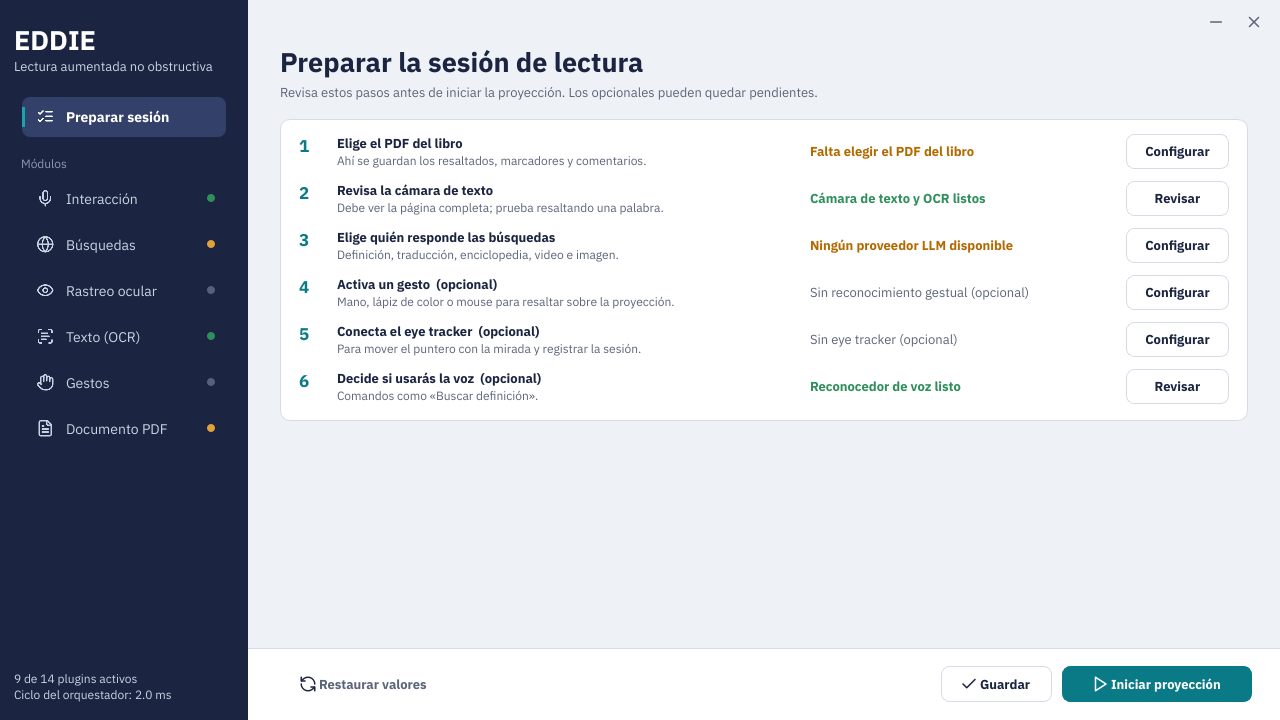
\includegraphics[width=0.85\textwidth]{figuras/00_menu_settings.png}
\caption{Pantalla de inicio con los pasos de preparación y el estado de cada módulo.}
\label{fig:ui_inicio}
\fuente{Elaboración propia (captura del avance P-07 con dispositivos simulados).}
\end{figure}

\begin{figure}[H]
\centering
\begin{minipage}{0.49\textwidth}\centering
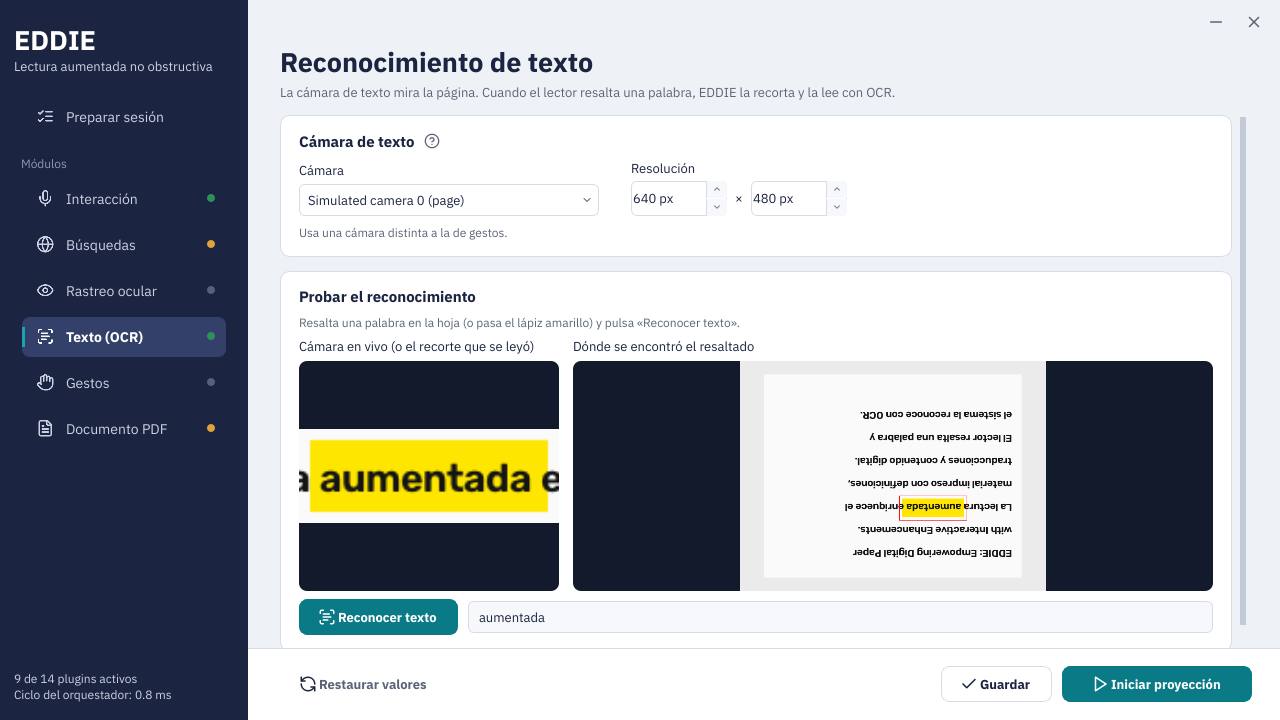
\includegraphics[width=\linewidth]{figuras/01_text.png}
\end{minipage}\hfill
\begin{minipage}{0.49\textwidth}\centering
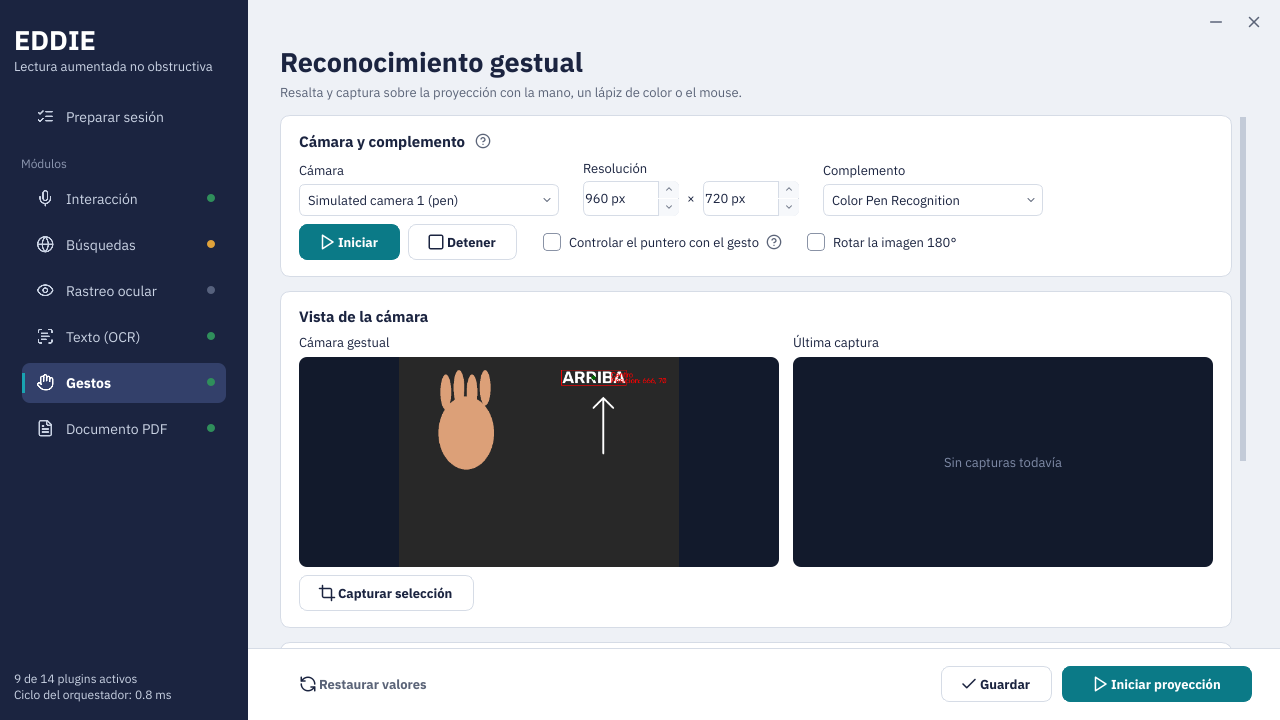
\includegraphics[width=\linewidth]{figuras/03_gesture_lapiz.png}
\end{minipage}
\caption{Configuración del reconocimiento de texto (izquierda) y de la interacción gestual con lápiz (derecha).}
\label{fig:ui_texto_gestos}
\fuente{Elaboración propia (capturas del avance P-07).}
\end{figure}

\begin{figure}[H]
\centering
\begin{minipage}{0.49\textwidth}\centering
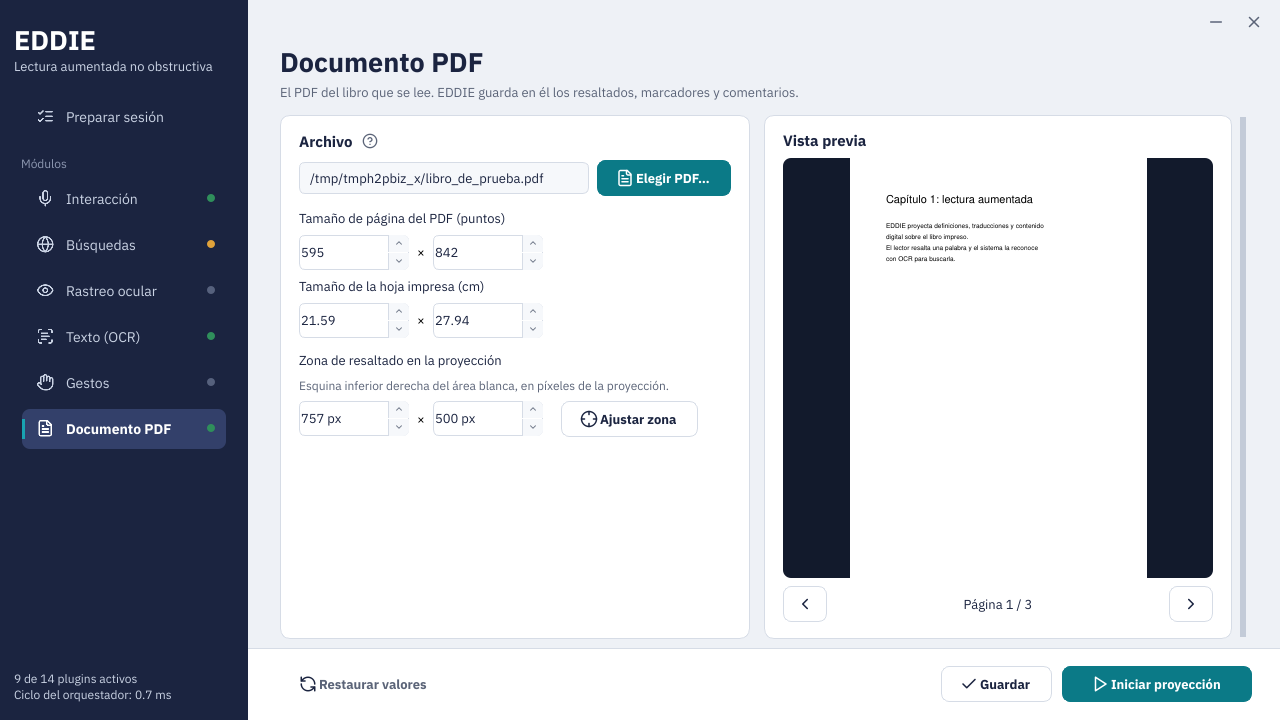
\includegraphics[width=\linewidth]{figuras/02_page.png}
\end{minipage}\hfill
\begin{minipage}{0.49\textwidth}\centering
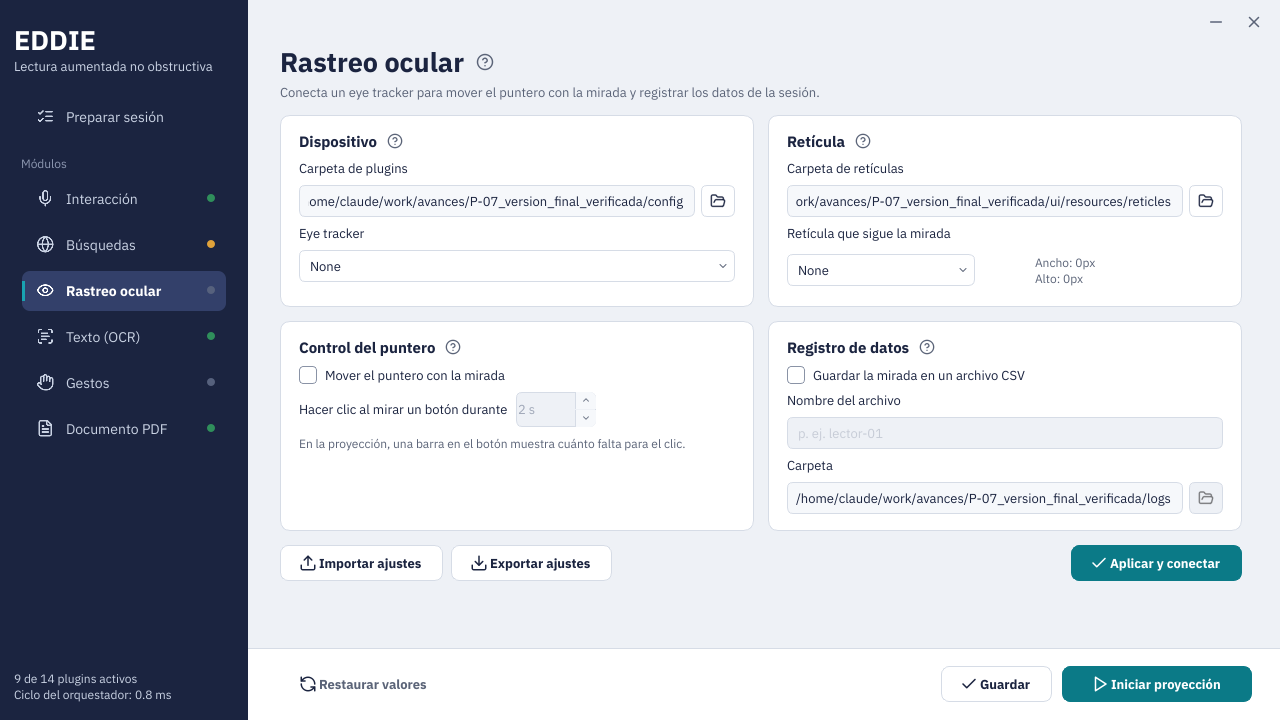
\includegraphics[width=\linewidth]{figuras/04_eye.png}
\end{minipage}
\caption{Configuración del documento PDF (izquierda) y del rastreo ocular (derecha).}
\label{fig:ui_pdf_ojo}
\fuente{Elaboración propia (capturas del avance P-07).}
\end{figure}

\begin{figure}[H]
\centering
\begin{minipage}{0.49\textwidth}\centering
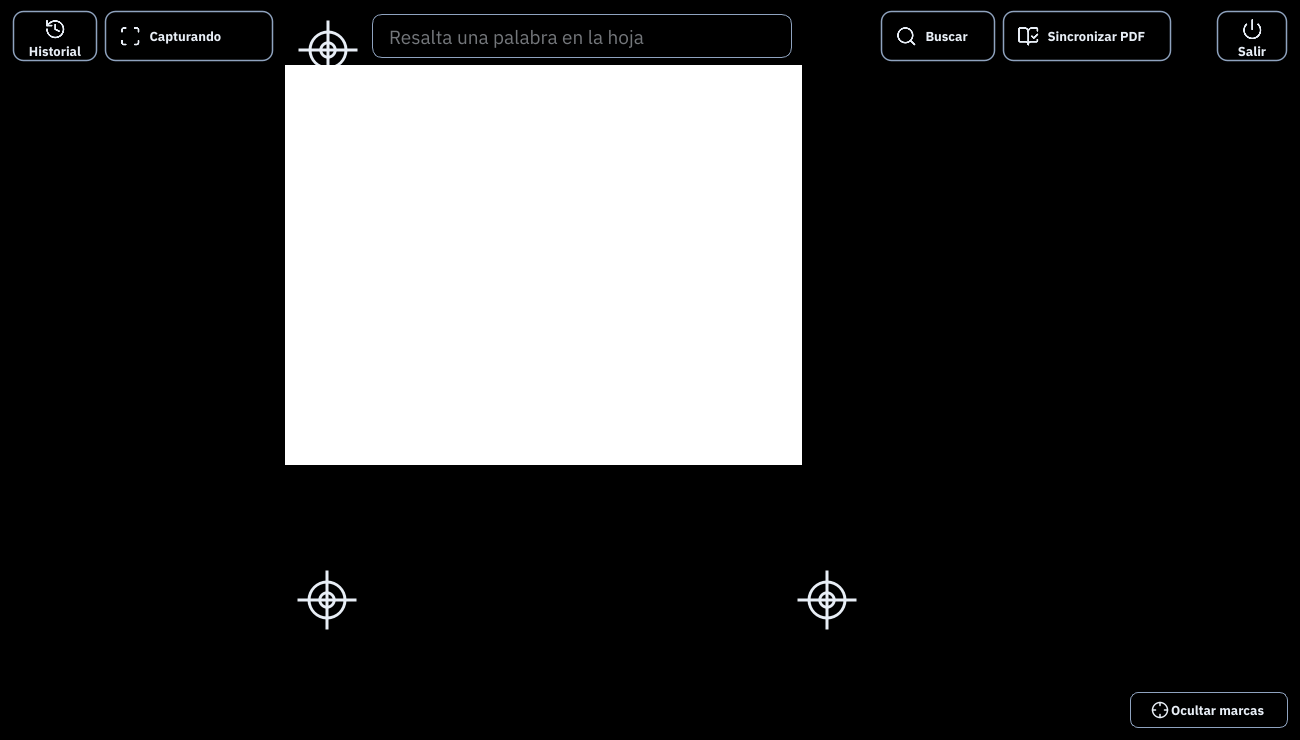
\includegraphics[width=\linewidth]{figuras/10_proyeccion.png}
\end{minipage}\hfill
\begin{minipage}{0.49\textwidth}\centering
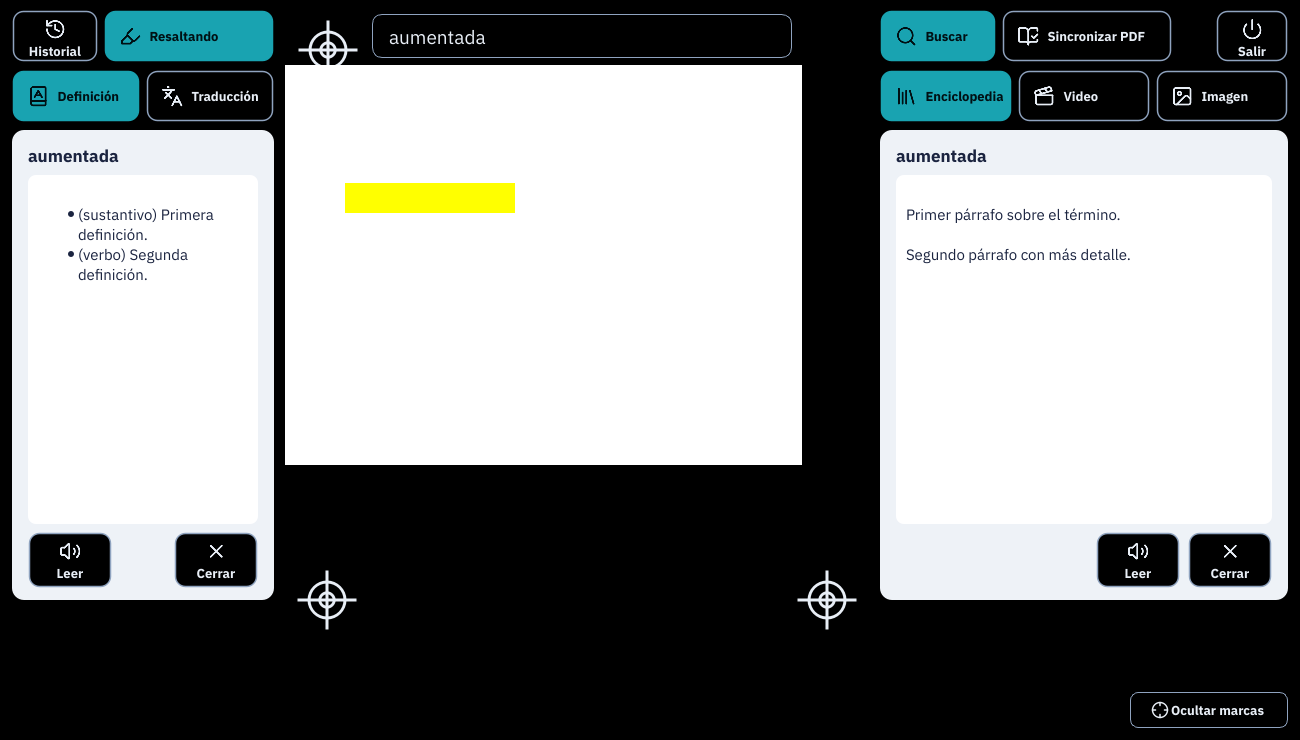
\includegraphics[width=\linewidth]{figuras/11_proyeccion_busqueda.png}
\end{minipage}
\caption{Pantalla proyectada: controles en la franja superior (izquierda) y resultado de una búsqueda (derecha).}
\label{fig:ui_proyeccion}
\fuente{Elaboración propia (capturas del avance P-07 con un modelo de lenguaje de prueba).}
\end{figure}

\section{Iteraciones de desarrollo}

El sistema se construyó en ocho avances, cada uno con su código completo, pruebas y evidencias reproducibles (Tabla~\ref{tab:avances}). P-00 corresponde a los prototipos desechables del Capítulo~\ref{cap:analisis}; P-01 a P-06 integran el núcleo y los módulos en el orden de menor a mayor dependencia del hardware; P-07 es la versión verificada. La interfaz se incorpora desde P-03 y muestra, en cada avance, solo los módulos ya integrados: los demás aparecen deshabilitados con la etiqueta del avance en que se integran. Las fichas de cada avance, con sus objetivos y requisitos, están en el Apéndice~\ref{ap:avances}.

\begin{table}[H]
\centering
\caption{Avances del desarrollo y resultados de sus pruebas.}
\label{tab:avances}
\footnotesize
\begin{tabularx}{\textwidth}{l >{\raggedright\arraybackslash}X c c c c}
\toprule
\textbf{Avance} & \textbf{Contenido} & \textbf{PDCA} & \textbf{Pruebas} & \textbf{Fallos esperados} & \textbf{Cobertura} \\ \midrule
P-00 & Prototipos desechables y mediciones & Plan & --- & --- & --- \\
P-01 & Núcleo orquestador y contratos & Do & \PUnoPruebas & \PUnoXfail & \PUnoCobertura\% \\
P-02 & Capa de hardware y consistencia & Do & \PDosPruebas & \PDosXfail & \PDosCobertura\% \\
P-03 & Reconocimiento de texto e interfaz & Do & \PTresPruebas & \PTresXfail & \PTresCobertura\% \\
P-04 & Interacción gestual & Do & \PCuatroPruebas & \PCuatroXfail & \PCuatroCobertura\% \\
P-05 & Rastreo ocular & Do & \PCincoPruebas & \PCincoXfail & \PCincoCobertura\% \\
P-06 & Proyección, búsqueda con LLM y voz & Do & \PSeisPruebas & \PSeisXfail & \PSeisCobertura\% \\
P-07 & Versión final verificada & Check/Act & \PSietePruebas & \PSieteXfail & \PSieteCobertura\% \\ \bottomrule
\end{tabularx}
\fuente{Elaboración propia a partir de \texttt{evidencias/} de cada avance.}
\end{table}

Los fallos esperados (\textit{xfail}) son pruebas que documentan un defecto conocido: en los avances en que el defecto existe la prueba se marca como fallo esperado, y en P-07, con la corrección aplicada, pasa a aprobada. Así cada corrección queda respaldada por una prueba que demuestra el problema y su solución (Sección~\ref{sec:hallazgos}).

\chapter{Evaluación}
\label{cap:evaluacion}

Este capítulo corresponde a la etapa \textit{Check} del ciclo PDCA y al cuarto objetivo específico. La evaluación se organiza en los tres niveles del diseño experimental de la propuesta: pruebas de software, verificación y validación con MECIVA PS, y pruebas de aceptación en el laboratorio. El primer nivel se ejecutó completo con dispositivos simulados; los dos siguientes requieren el hardware del laboratorio, y para ellos se presentan el protocolo, los instrumentos ya construidos y los resultados que faltan, marcados como \pendiente{laboratorio}.

\section{Plan de evaluación}

La Tabla~\ref{tab:plan_eval} resume las métricas comprometidas, su criterio de aceptación y su estado. Todas las métricas automatizadas se regeneran con \texttt{python tools/generar\_evidencias.py} en cada avance, y los resultados de este capítulo provienen de la carpeta \texttt{evidencias/} del avance P-07 (\PSieteEntorno, \PSieteFecha).

\begin{table}[H]
\centering
\caption{Métricas de evaluación, criterio de aceptación y estado.}
\label{tab:plan_eval}
\footnotesize
\begin{tabularx}{\textwidth}{>{\raggedright\arraybackslash}p{3.8cm} >{\raggedright\arraybackslash}X >{\raggedright\arraybackslash}p{3.2cm}}
\toprule
\textbf{Métrica} & \textbf{Criterio} & \textbf{Estado} \\ \midrule
\multicolumn{3}{l}{\textbf{Nivel 1: pruebas de software}} \\
Cobertura de líneas & $\geq$ 80\% (RNF-03) & \PSieteCobertura\%, cumple \\
Latencia orquestador $\rightarrow$ plugin & p95 $\leq$ 8,3~ms (RNF-01) & \PSieteCicloPnoventaycinco~ms el ciclo completo, cumple \\
Aislamiento de fallos & Una falla no detiene el sistema (RNF-02) & Verificado por pruebas \\
Matriz de trazabilidad & Cada caso: corregido, persistente o fuera de alcance & Parcial (Sección~\ref{sec:trazabilidad}) \\
Desfase entre sensores y pérdida de eventos & Desfase máximo (ms) y tasa de pérdida en captura simultánea & \pendiente{laboratorio} \\
Precisión y recall del OCR & $\geq$ 10 palabras de distinto largo & Métrica implementada; \pendiente{cámara} \\
Tasa de error gestual & Gestos bien clasificados / ejecutados & \pendiente{laboratorio} \\ \midrule
\multicolumn{3}{l}{\textbf{Nivel 2: verificación y validación (MECIVA PS)}} \\
Requisitos críticos & 100\% de las ejecuciones & \pendiente{laboratorio} \\
Validez funcional & \% de requisitos heredados cumplidos & \pendiente{laboratorio} \\
Confiabilidad & CV o tasa de éxito, $\geq$ 10 ejecuciones por caso & \pendiente{laboratorio} \\ \midrule
\multicolumn{3}{l}{\textbf{Nivel 3: pruebas de aceptación}} \\
Requisitos secundarios & Escala A--E (Tabla~\ref{tab:escala}) & \pendiente{laboratorio} \\ \bottomrule
\end{tabularx}
\fuente{Elaboración propia a partir de la propuesta de tesis.}
\end{table}

\section{Pruebas de software}

\subsection{Pruebas automatizadas y cobertura}

La versión final tiene \PSietePruebas{} pruebas automatizadas con pytest, organizadas en cinco archivos: núcleo y cargador (\texttt{test\_orchestrator.py}), hardware y núcleo extendido (\texttt{test\_hardware\_and\_core.py}), contratos y plugins (\texttt{test\_plugins\_eddie.py}), flujos de la interfaz (\texttt{test\_ui\_flows.py}) e interfaz rediseñada (\texttt{test\_interfaz.py}). Las pruebas de interfaz ejecutan los flujos reales de la aplicación (abrir un PDF, sincronizar un resaltado, calibrar un gesto, abrir la proyección) con dispositivos simulados y sin pantalla. Todas aprueban y la cobertura de líneas es de \PSieteCobertura\%, sobre el umbral de 80\% comprometido.

La Tabla~\ref{tab:avances} (Capítulo~\ref{cap:diseno}) muestra la evolución por avance. La cobertura de P-02 a P-05 está bajo el umbral porque esos avances contienen código de interfaz o de dispositivos que todavía no tenía pruebas de flujo completas; el umbral se exige a la versión final, que es la que se entrega.

\subsection{Latencia del orquestador}

Se midieron \PSieteCiclos{} ciclos completos del orquestador, tras 10 de calentamiento, con todos los plugins activos y el reconocimiento con lápiz encendido (Tabla~\ref{tab:latencias}). El ciclo completo, que incluye a todos los plugins, tiene una latencia de \PSieteCicloMedia~ms en promedio y \PSieteCicloPnoventaycinco~ms en el percentil 95, con un máximo de \PSieteCicloMax~ms. Ningún plugin superó los 8,3~ms en ningún ciclo, por lo que RNF-01 se cumple con margen: el ciclo completo usa menos del 10\% del período entre dos muestras del eye tracker.

\begin{table}[H]
\centering
\caption{Latencia por plugin en \PSieteCiclos{} ciclos del orquestador (ms).}
\label{tab:latencias}
\small
\begin{tabular}{lrrr}
\toprule
\textbf{Plugin} & \textbf{Media} & \textbf{p95} & \textbf{Máx.} \\ \midrule
\PSieteTablaLatencias \\ \midrule
\textbf{Ciclo completo} & \PSieteCicloMedia & \PSieteCicloPnoventaycinco & \PSieteCicloMax \\ \bottomrule
\end{tabular}
\fuente{Elaboración propia, \texttt{evidencias/latencias.json} de P-07 (dispositivos simulados).}
\end{table}

Dos limitaciones acotan este resultado. Primero, se midió con dispositivos simulados: la latencia de captura de la cámara real y la del eye tracker ocurren en hilos propios y no forman parte del ciclo, pero el costo del reconocimiento sobre imágenes reales puede ser mayor. Segundo, en P-06 se registró un ciclo aislado de 10,28~ms con un percentil 95 de 1,49~ms; corresponde a una pausa del sistema operativo o del recolector de memoria y no se repitió en P-07, pero muestra que el máximo debe medirse también en el PC del laboratorio con \texttt{generar\_evidencias.py --real}.

\subsection{Aislamiento de fallos}

El aislamiento de fallos (RNF-02) se verifica con pruebas que provocan fallas en cada fase del ciclo de vida: una clase que no existe o un módulo inválido (\texttt{test\_load\_invalid\_module}, \texttt{test\_load\_all\_missing\_class\_key}), un archivo de configuración ausente (\texttt{test\_initialize\_with\_missing\_config\_file}), un plugin cuya inicialización falla (\texttt{test\_initialize\_plugin\_init\_fail\_does\_not\_stop\_system}), una excepción en \texttt{execute()} (\texttt{test\_execute\_plugin\_exception\_isolation}), una excepción al liberar (\texttt{test\_release\_exception\_does\_not\_stop\_others}) y una operación bajo demanda que falla (\texttt{test\_invoke\_isolates\_failures}). En todos los casos el resto de los plugins sigue funcionando y la falla queda registrada con su causa.

El informe de inicialización de P-07 muestra el mismo comportamiento en la aplicación real: sin clave de Gemini configurada, el plugin de búsqueda queda como \texttt{initialization\_failed} y los otros trece plugins se inicializan normalmente. En EDDIE-2023, una situación equivalente (una DLL o carpeta de plugins faltante, E50) impedía usar el módulo completo.

\subsection{Matriz de trazabilidad}
\label{sec:trazabilidad}

La propuesta compromete reejecutar los casos de prueba documentados por \citet{pezoa2020}, \citet{contreras2019} y \citet{estay2020} en EDDIE-2023 y en la versión en Python, y registrar cada error de \citet{ibaceta2023} como corregido, persistente o fuera de alcance, con su evidencia. La Tabla~\ref{tab:trazabilidad} presenta la parte de la matriz que puede respaldarse con pruebas automatizadas; los casos que dependen del hardware quedan como pendientes hasta su ejecución en el laboratorio. La matriz completa de los 67 errores se construye con la plantilla del Anexo~\ref{an:errores}.

\begin{table}[H]
\centering
\caption{Matriz de trazabilidad (parcial) de errores de EDDIE-2023.}
\label{tab:trazabilidad}
\scriptsize
\begin{tabularx}{\textwidth}{>{\raggedright\arraybackslash}p{1.5cm} >{\raggedright\arraybackslash}p{3.1cm} c >{\raggedright\arraybackslash}p{2.3cm} >{\raggedright\arraybackslash}X}
\toprule
\textbf{Error} & \textbf{Descripción} & \textbf{Cat.} & \textbf{Resultado} & \textbf{Evidencia} \\ \midrule
E50 & Carpeta \texttt{PluginsConsistencia} no encontrada & (a) & Corregido por diseño & \texttt{test\_load\_invalid\_module}, \texttt{test\_load\_all\_missing\_class\_key} \\ \midrule
E7, E8 & No inicia sin cámara o sin dos cámaras & (d) & Corregido & \texttt{test\_camera\_sensor\_fails\_cleanly\_when\_camera\_missing}; modo simulado \\ \midrule
E11, E21, E22, E30 & Fallas al sincronizar, buscar o revisar sin PDF o sin página & (d) & Corregido & \texttt{test\_missing\_pdf\_is\_reported\_not\_crashing}, \texttt{test\_pdf\_tools\_require\_pdf\_and\_page\_number} \\ \midrule
E12, E13 & Sin manual de instalación ni de uso & (c) & Corregido & README del repositorio y manual del Apéndice~\ref{ap:manual} \\ \midrule
E14 & Mensajes en otro idioma & (e) & Corregido & Interfaz y mensajes en español (RNF-06) \\ \midrule
EFD2 & La cámara detecta botones de la interfaz & (e) & Corregido por diseño; \pendiente{verificar con cámara} & \texttt{test\_interface\_chrome\_never\_uses\_yellow} \\ \midrule
E27, E28 & Código sin comentarios ni nombres representativos & (d) & \pendiente{SonarQube} & Docstrings y análisis estático \\ \midrule
E40, E41 & Resaltado digital no coincide con el físico & (d) & \pendiente{laboratorio} & Prueba de aceptación de consistencia \\ \midrule
E15, E16 & Eye tracker no reconocido; cámara inestable & (b) & \pendiente{laboratorio} & Modo real vs.\ simulado (DeviceFactory) \\ \midrule
E49 & No se detecta la parte inferior de la proyección & (b) & Mitigado por diseño; \pendiente{laboratorio} & Controles en la franja superior; prueba con GazePoint \\ \midrule
APIs de búsqueda & Credenciales vencidas & (g) & Corregido por reemplazo & \texttt{test\_gemini\_key\_from\_secrets\_file\_or\_missing} y servidor de prueba \\ \midrule
E9, E10 & Conexiones eléctricas y seguridad del equipo & (f) & Fuera de alcance & Infraestructura del laboratorio \\ \bottomrule
\end{tabularx}
\fuente{Elaboración propia a partir de \citet{ibaceta2023} y de las pruebas de P-07. Categorías de la Tabla~\ref{tab:reclasificacion}: (a) carga y despliegue, (b) hardware, (c) documentación, (d) práctica de código, (e) interfaz e idioma, (f) infraestructura, (g) servicios externos.}
\end{table}

\subsection{Hallazgos de la verificación}
\label{sec:hallazgos}

Durante el desarrollo y la verificación se encontraron tres defectos que las pruebas automatizadas no habían detectado. Cada uno se documentó con una prueba que lo reproduce y se corrigió (Tabla~\ref{tab:hallazgos_verif}).

\begin{table}[H]
\centering
\caption{Hallazgos de la verificación y su corrección.}
\label{tab:hallazgos_verif}
\footnotesize
\begin{tabularx}{\textwidth}{>{\raggedright\arraybackslash}p{1.1cm} >{\raggedright\arraybackslash}X >{\raggedright\arraybackslash}X}
\toprule
\textbf{ID} & \textbf{Problema} & \textbf{Corrección y prueba} \\ \midrule
H-01 & Al calibrar con la mano la imagen aparecía rotada 180°: el plugin heredó de \texttt{HandSkinRecognition.cs} una rotación fija pensada para la cámara invertida del laboratorio. & La rotación pasa a ser una opción común de los tres plugins gestuales, desactivada por defecto, con una casilla en la interfaz. Pruebas \texttt{test\_gesture\_preview\_keeps\_camera\_orientation\_by\_default} y relacionadas. \\ \midrule
H-02 & Con PyMuPDF 2.1, desde el segundo guardado incremental el PDF quedaba con su tabla de referencias dañada y al reabrirlo se perdían anotaciones. & Cada guardado escribe una copia completa y reemplaza el original, con reintento si el archivo está bloqueado. Pruebas \texttt{test\_successive\_saves\_keep\_every\_annotation\_on\_disk} y relacionadas. \\ \midrule
H-03 & Los botones de ayuda de Rastreo ocular lanzaban una excepción en cada clic porque la señal de Qt reemplazaba el argumento del \textit{callback}. & La función ignora los argumentos de la señal. Prueba \texttt{test\_info\_icons\_and\_buttons\_with\_help\_do\_not\_raise}. \\ \bottomrule
\end{tabularx}
\fuente{Elaboración propia.}
\end{table}

Los tres hallazgos tienen un rasgo común: el programa parecía funcionar. En H-02 el documento en memoria era correcto y el daño solo aparecía al reabrir el archivo; en H-03 la acción del botón se ejecutaba y la excepción quedaba en el registro. Esto refuerza la necesidad de las pruebas de aceptación con el hardware real, porque hay defectos que solo se observan al operar el sistema completo.

\section{Verificación y validación con MECIVA PS}

\subsection{Protocolo}

La verificación replica la fase de diagnóstico de MECIVA PS \citep{ibaceta2023} para cada módulo del MVP: consistencia, reconocimiento de texto, interacción gestual y rastreo ocular. Para cada módulo:

\begin{enumerate}
  \item Se clasifican sus requisitos en \textbf{críticos}, que deben cumplirse en el 100\% de las ejecuciones y cuyo incumplimiento es bloqueante (por ejemplo, que los plugins del MVP carguen sin fallas, o que el error espacial del rastreo ocular esté dentro del margen definido), y \textbf{secundarios}, que se evalúan con la escala de la Tabla~\ref{tab:escala}.
  \item Se ejecuta cada caso al menos 10 veces con el hardware real (\texttt{EDDIE\_DEVICE\_MODE=real}) y se registra el resultado en la plantilla de diagnóstico de MECIVA PS (funcionalidad, resultado esperado, método, pruebas, resultados y nivel de funcionamiento).
  \item Se calcula la \textbf{validez funcional} como el porcentaje de requisitos heredados que el módulo cumple, y la \textbf{confiabilidad} como el coeficiente de variación $\mathrm{CV}=\sigma/\mu$ para variables continuas (por ejemplo, las coordenadas de una fijación sobre un punto fijo) o como la tasa de éxito para resultados binarios (por ejemplo, que un comentario se sincronice).
\end{enumerate}

Para el reconocimiento de texto se usa el mismo conjunto de \citet{ibaceta2023}: diez palabras de distinto largo (Control, Arte, Lectura, Jerusalén, Esponja, Pastilla, Caramelo, Metodología, Consistencia y Cama) en nueve posiciones de la zona de lectura, con diez repeticiones por posición. Así los resultados son directamente comparables con la línea base de 2023, en que la validez varió entre 10\% y 100\% según la posición. El plugin calcula precisión y recall con \texttt{get\_precision\_recall} (verificado en \texttt{test\_precision\_recall\_metric}):
\begin{equation}
\mathrm{Precisión}=\frac{|P_{\text{reconocidas}}\cap P_{\text{esperadas}}|}{|P_{\text{reconocidas}}|},\qquad
\mathrm{Recall}=\frac{|P_{\text{reconocidas}}\cap P_{\text{esperadas}}|}{|P_{\text{esperadas}}|}.
\end{equation}

\subsection{Resultados}

\pendiente{Tabla de validez y confiabilidad por módulo, con la línea base de \citet{ibaceta2023} en una columna para comparar.}

\section{Pruebas de aceptación}

Las pruebas de aceptación se realizan en la sala del laboratorio InTeractiOn con el profesor guía como evaluador, siguiendo la práctica de los trabajos anteriores del laboratorio \citep{estay2020,pezoa2020,figueroa2025}. Cada prueba tiene precondiciones, pasos, requisitos abordados y resultado esperado, y se califica con la escala de la Tabla~\ref{tab:escala}. Los escenarios cubren la operación simultánea de módulos, la recuperación ante la falla parcial de un sensor (desconectar una cámara durante la sesión) y la sincronización de datos entre componentes de frecuencias distintas.

\begin{table}[H]
\centering
\caption{Escala de evaluación de las pruebas de aceptación.}
\label{tab:escala}
\small
\begin{tabular}{clc}
\toprule
\textbf{Evaluación} & \textbf{Significado} & \textbf{Cumplimiento} \\ \midrule
A & Completa & 85--100\% \\
B & Aceptada con observaciones & 55--84,9\% \\
C & Incompleta & 45--54,9\% \\
D & Insuficiente & 15--44,9\% \\
E & No aceptada & 0--14,9\% \\ \bottomrule
\end{tabular}
\fuente{\citet{estay2020}.}
\end{table}

\begin{table}[H]
\centering
\caption{Pruebas de aceptación planificadas.}
\label{tab:aceptacion}
\footnotesize
\begin{tabularx}{\textwidth}{l >{\raggedright\arraybackslash}X >{\raggedright\arraybackslash}p{3.2cm} c}
\toprule
\textbf{ID} & \textbf{Prueba} & \textbf{Requisitos} & \textbf{Resultado} \\ \midrule
PA-01 & Arrancar con todos los plugins del MVP, desconectar una cámara durante la sesión y reconectarla desde la interfaz. & N1, N2, N6, RNF-02 & \pendiente{} \\
PA-02 & Resaltar una palabra en el papel y obtener su texto, su definición y su traducción. & FD1, B1--B13 & \pendiente{} \\
PA-03 & Sincronizar resaltado, comentario, marcador y figura del papel al PDF y del PDF al papel. & C1--C12 & \pendiente{} \\
PA-04 & Calibrar el lápiz y la mano, seleccionar un fragmento y capturarlo. & G1--G3, U2 & \pendiente{} \\
PA-05 & Conectar GazePoint y TheEyeTribe, ver la retícula y activar un botón de la proyección con la mirada. & RO1--RO7 & \pendiente{} \\
PA-06 & Registrar una sesión de lectura y verificar el CSV de mirada y la traza del orquestador. & RO4, N7 & \pendiente{} \\
PA-07 & Preparar una sesión completa desde la pantalla de inicio siguiendo el manual. & U1, U3, RFS1--RFS8 & \pendiente{} \\ \bottomrule
\end{tabularx}
\fuente{Elaboración propia.}
\end{table}

\section{Síntesis de la evaluación}

Las pruebas de software muestran que la arquitectura cumple los requisitos no funcionales que pueden verificarse sin el laboratorio: cobertura de \PSieteCobertura\% (RNF-03), latencia del ciclo completo de \PSieteCicloPnoventaycinco~ms en el percentil 95 (RNF-01), aislamiento de fallos en todas las fases del ciclo de vida (RNF-02), extensibilidad por configuración (RNF-04) y ejecución completa con dispositivos simulados (RNF-05). De los errores de EDDIE-2023, los de carga y despliegue, práctica de código, documentación e idioma que se pudieron reproducir quedan corregidos y respaldados por pruebas. Los errores de hardware y la coincidencia física del resaltado (E40, E41, E49) solo pueden cerrarse con las pruebas del laboratorio, para las que el protocolo y los instrumentos de medición ya están disponibles.

\chapter{Conclusiones}
\label{cap:conclusiones}

\textit{Versión preliminar: las conclusiones sobre el cuarto objetivo se completan con los resultados de la verificación funcional y de las pruebas de aceptación en el laboratorio.}

\section{Cumplimiento de los objetivos}

\paragraph{OE1: diagnóstico y factibilidad.} La reclasificación por causa de los 67 errores de \citet{ibaceta2023} mostró que 42 de ellos (62,7\%) dependen de la arquitectura (carga y despliegue, y práctica de código) y no del hardware, lo que justifica reconstruir el núcleo en lugar de corregir errores aislados. Los 19 prototipos desechables confirmaron que las funciones críticas pueden reproducirse en Python con bibliotecas mantenidas y, al medirse con verdad terreno conocida, entregaron cinco hallazgos que no eran visibles en el código del sistema legado: la binarización global falla con la luz del proyector, el preprocesamiento empeora el OCR sobre texto limpio, el contenido proyectado del color del lápiz anula su seguimiento, el orden de la regla de clasificación de figuras confunde cuadrados con círculos y el clic por permanencia depende fuertemente del ruido del sensor. El objetivo se considera cumplido, con las mediciones que dependen del hardware (F1, F9, F24, F25 y la parte de sensor de las demás) pendientes de ejecutar en el laboratorio con el mismo script.

\paragraph{OE2: diseño del núcleo.} Se definió un contrato base único (\texttt{PluginBase}) con ciclo de inicialización, ejecución y liberación, siete contratos de dominio y dos interfaces de flujo de datos, un único archivo de configuración y una capa de abstracción de hardware con conmutación real/simulado. El diseño reemplaza los tres mecanismos de carga de EDDIE-2023 por uno solo. El objetivo se considera cumplido.

\paragraph{OE3: implementación e integración.} Se implementó el núcleo y se integraron, en siete iteraciones, los módulos de consistencia, reconocimiento de texto, interacción gestual (lápiz, mano y mouse), rastreo ocular (GazePoint, TheEyeTribe, GazeCloud y simulado), búsqueda con modelo de lenguaje y voz, junto con la interfaz de configuración y la pantalla proyectada. La interfaz conserva todos los controles y flujos de EDDIE-2023 y corrige los problemas de usabilidad registrados en 2023. El objetivo se considera cumplido en software; la integración con el hardware físico se confirma en las pruebas de aceptación.

\paragraph{OE4: validación.} Las pruebas de software se completaron: \PSietePruebas{} pruebas aprobadas, \PSieteCobertura\% de cobertura de líneas, latencia del ciclo completo de \PSieteCicloPnoventaycinco~ms en el percentil 95 frente al umbral de 8,3~ms y aislamiento de fallos verificado en todas las fases del ciclo de vida. La verificación funcional con MECIVA PS y las pruebas de aceptación \pendiente{se ejecutan en el laboratorio}; sus protocolos e instrumentos están listos (Capítulo~\ref{cap:evaluacion}).

\section{Respuesta a la pregunta de investigación}

La pregunta planteada fue en qué medida la reconstrucción del núcleo bajo una arquitectura de plugins con contrato único permite reducir los errores estructurales documentados y habilitar el uso de EDDIE como instrumento de medición confiable. Respecto de la primera parte, los errores de carga y despliegue dejan de ser posibles por construcción: un plugin faltante o defectuoso se registra y el resto del sistema arranca, y los errores de práctica de código que se reprodujeron quedan respaldados por pruebas. Respecto de la segunda, la arquitectura entrega las condiciones necesarias para medir (latencia acotada, traza de cada acción, ejecución reproducible con dispositivos simulados), pero la confiabilidad de las mediciones con el hardware real solo puede afirmarse después de la verificación con MECIVA PS.

\section{Limitaciones}

\begin{itemize}
  \item Los resultados de los prototipos marcados como sintéticos miden el algoritmo sobre datos con verdad terreno conocida, no el desempeño con la cámara o el eye tracker reales.
  \item Las pruebas de software se ejecutaron con dispositivos simulados; la latencia y el comportamiento con el hardware real deben medirse en el PC del laboratorio.
  \item La búsqueda depende de un servicio externo (Gemini) y de una clave personal; si el servicio cambia sus condiciones, el contrato \texttt{IWebSearchProvider} permite reemplazarlo, pero el reemplazo no está implementado.
  \item El desarrollo y la validación se realizan solo en Windows~11.
\end{itemize}

\section{Trabajo futuro}

\begin{itemize}
  \item Ejecutar la verificación con MECIVA PS y las pruebas de aceptación, y completar la matriz de trazabilidad de los 67 errores.
  \item Calibrar los parámetros del clic por permanencia y los umbrales de color con el hardware del laboratorio.
  \item Implementar un proveedor de búsqueda local (por ejemplo, un modelo de lenguaje ejecutado en el equipo) para no depender de un servicio externo.
  \item Retomar la detección automática del libro (F4), que resultó factible, y el canal de telemetría para el visor web que quedó fuera del alcance.
\end{itemize}

\chapter*{GLOSARIO}
\addcontentsline{toc}{chapter}{Glosario}

\begin{description}
  \item[Arquitectura de plugins:] organización de un sistema en un núcleo estable y módulos intercambiables que implementan un contrato común y se pueden agregar o reemplazar sin modificar el núcleo.
  \item[Capa de abstracción de hardware (HAL):] componente que oculta los detalles de cada dispositivo detrás de una interfaz uniforme, de modo que un dispositivo real puede reemplazarse por uno simulado.
  \item[Clic por permanencia (\textit{dwell}):] activación de un control cuando la mirada permanece dentro de un radio durante un tiempo mínimo.
  \item[Consistencia bidireccional:] en EDDIE, mantener equivalentes el documento impreso y su versión PDF, de modo que una marca hecha en uno se refleje en el otro.
  \item[Contrato de interfaz:] conjunto de operaciones que un módulo se compromete a implementar; en este trabajo, una clase abstracta de Python.
  \item[Deuda técnica:] costo futuro de retrabajo derivado de elegir soluciones rápidas en lugar de un diseño mantenible.
  \item[Eye tracker:] dispositivo que estima, a una frecuencia fija, el punto al que mira una persona.
  \item[Fijación:] período en que la mirada permanece estable sobre una región.
  \item[Homografía:] transformación proyectiva entre dos planos, usada para convertir coordenadas de la cámara en coordenadas de la proyección.
  \item[Interacción humano-información (HII):] campo que estudia cómo las personas buscan, evalúan y usan información en distintos formatos.
  \item[Latencia:] tiempo entre una acción y su resultado; en este trabajo, el tiempo que el orquestador tarda en ejecutar un plugin o un ciclo completo.
  \item[MECIVA PS:] metodología para la evaluación y validación de productos de software desarrollados para EDDIE \citep{ibaceta2023}.
  \item[Modelo de lenguaje (LLM):] modelo de aprendizaje automático que genera texto a partir de una instrucción; en EDDIE responde los servicios de búsqueda.
  \item[OCR:] reconocimiento óptico de caracteres; conversión de la imagen de un texto en caracteres.
  \item[Orquestador:] componente central que controla el ciclo de vida de los plugins y coordina el flujo de datos entre ellos.
  \item[Percentil 95 (p95):] valor bajo el cual queda el 95\% de las mediciones.
  \item[Prototipo desechable:] pieza de software acotada que se construye para evaluar la factibilidad de una función y luego se descarta.
  \item[QuadPoints:] coordenadas de los cuatro vértices de cada fragmento de texto en un PDF, usadas para resaltarlo.
  \item[Realidad aumentada espacial:] superposición de información digital directamente sobre los objetos físicos mediante un proyector.
  \item[\textit{Science gateway}:] plataforma que integra instrumentos, datos y flujos de trabajo científicos.
  \item[Software científico:] software desarrollado \textit{ad hoc} para soportar una tarea de investigación.
  \item[SonarQube:] plataforma de análisis estático de la calidad, la seguridad y la mantenibilidad del código.
  \item[Toque de Midas:] activación involuntaria de controles por el solo hecho de mirarlos.
\end{description}


\bibliographystyle{apalike}
\bibliography{referencias}

\appendix
% ============================================================================ ANEXOS
% Anexo = material de terceros o de la propuesta; Apéndice = elaboración propia.
\titleformat{\chapter}[hang]{\normalfont\Large\bfseries\raggedright}{ANEXO \thechapter.}{0.5em}{\MakeUppercase}

\chapter{Errores de EDDIE-2023 y plantilla de trazabilidad}
\label{an:errores}

La Tabla~\ref{tab:extracto_errores} reproduce un extracto de los errores registrados por \citet{ibaceta2023} que se citan en este documento. La matriz completa se construye con la plantilla de la Tabla~\ref{tab:plantilla_traz}, una fila por cada uno de los 67 errores, ejecutando el caso de prueba original en EDDIE-2023 y en la versión en Python.

\begin{table}[H]
\centering
\caption{Extracto de errores encontrados en EDDIE-2023.}
\label{tab:extracto_errores}
\footnotesize
\begin{tabularx}{\textwidth}{l l X c}
\toprule
\textbf{ID} & \textbf{Tipo} & \textbf{Descripción} & \textbf{Estado} \\ \midrule
E7 & Interno-otro & El programa no se puede inicializar por falta de cámara disponible. & SF \\
E8 & Interno-otro & El programa no funciona correctamente sin dos cámaras disponibles. & SF \\
E9 & Externo & Falta de conexiones eléctricas en el laboratorio. & SP \\
E10 & Externo & Falta de seguridad en el computador del laboratorio. & SF \\
E11 & Interno-consistencia & La sincronización hace fallar el programa cuando no se ingresa un PDF. & SF \\
E12 & Externo & No existe un manual de instalación. & SS \\
E13 & Externo & No existe un manual de uso. & SS \\
E14 & Interno-otro & Los mensajes de error están en un idioma distinto al resto de la aplicación. & SF \\
E15 & Externo & No se reconoce el eye tracker en el computador. & SF \\
E16 & Externo & La conexión de la cámara digital es inestable. & SP \\
E21 & Interno-consistencia & El botón de búsqueda hace fallar el programa si no se sube un PDF. & SF \\
E22 & Interno-consistencia & La revisión del contenido del PDF falla si no existe el archivo. & SF \\
E27 & Interno-otro & Faltan comentarios en el código. & SS \\
E28 & Interno-otro & Variables y funciones sin nombres representativos. & SS \\
E30 & Interno-consistencia & El contenido del PDF falla si no se indica una página. & SF \\
E48 & Interno-consistencia & La consistencia de comentarios falla con datos correctos. & SF \\
E49 & Externo & Con TheEyeTribe no se detecta la parte inferior de la proyección. & SS \\
E50 & Interno-consistencia & No se encuentra la carpeta \texttt{PluginsConsistencia}. & SF \\ \bottomrule
\end{tabularx}
\fuente{\citet{ibaceta2023}. SF: solución final; SP: solución parcial; SS: sin solución.}
\end{table}

\begin{table}[H]
\centering
\caption{Plantilla de la matriz de trazabilidad.}
\label{tab:plantilla_traz}
\footnotesize
\begin{tabularx}{\textwidth}{l l c c c >{\raggedright\arraybackslash}X >{\raggedright\arraybackslash}X}
\toprule
\textbf{ID} & \textbf{Módulo} & \textbf{Estado C\#} & \textbf{Cat.} & \textbf{¿Reproducido?} & \textbf{Resultado en Python} & \textbf{Evidencia} \\ \midrule
E\textit{n} & \dots & SF/SP/SS & (a)--(g) & Sí/No & Corregido / Persiste / Fuera de alcance & Prueba, log o nota de alcance \\ \bottomrule
\end{tabularx}
\fuente{Propuesta de tesis (Tabla 3.3).}
\end{table}

\chapter{Plan de trabajo}
\label{an:plan}

\begin{table}[H]
\centering
\caption{Plan de trabajo.}
\label{tab:plan_trabajo}
\footnotesize
\begin{tabularx}{\textwidth}{l l >{\raggedright\arraybackslash}X c c >{\raggedright\arraybackslash}p{3cm}}
\toprule
\textbf{Semanas} & \textbf{Fase} & \textbf{Actividades} & \textbf{OE} & \textbf{Horas} & \textbf{Entregable} \\ \midrule
1--3 & Plan & Diagnóstico de la arquitectura en C\# mediante la reclasificación de errores y prototipos desechables de factibilidad. & OE1 & 108 & Diagnóstico y resultados de prototipos \\ \midrule
4--6 & Do (diseño) & Diseño del núcleo y de los contratos de interfaz; primer prototipo funcional. & OE2 & 108 & Arquitectura y contratos \\ \midrule
7--10 & Do (implem.) & Núcleo, capa de abstracción de sensores, consistencia, reconocimiento de texto e interacción gestual. & OE3 & 144 & Prototipos funcionales del núcleo con módulos \\ \midrule
11--12 & Do (implem.) & Rastreo ocular con hardware físico; contingencia: validación con \texttt{EyeTrackerMock}. & OE3 & 72 & Prototipo integrado \\ \midrule
13--14 & Check & Pruebas de software: cobertura, trazabilidad, latencia y métricas de sincronización y visión. & OE4 & 72 & Reporte de pruebas de software \\ \midrule
15--16 & Check & MECIVA PS por módulo, validez y confiabilidad, pruebas de aceptación. & OE4 & 72 & Reporte de verificación y validación \\ \midrule
17 & Act & Ajustes finales, cierre de la documentación y entrega. & OE4 & 36 & Documentación y entrega final \\ \bottomrule
\end{tabularx}
\fuente{Propuesta de tesis (Tabla 6.1).}
\end{table}

% ============================================================================ APÉNDICES
\titleformat{\chapter}[hang]{\normalfont\Large\bfseries\raggedright}{APÉNDICE \thechapter.}{0.5em}{\MakeUppercase}
\setcounter{chapter}{0}

\chapter{Fichas de los avances}
\label{ap:avances}

Cada avance se describe con el formato de \citet{figueroa2025}: identificador, nombre, objetivos, descripción y requisitos funcionales y no funcionales. Las tablas se generan desde la carpeta \texttt{avances/} del repositorio.

{\small% Tablas de prototipos de EDDIE (formato de Figueroa Contreras, 2025). Requiere \usepackage{tabularx}.
% Generado desde avances/; revisa los códigos de requisitos antes de usarlos.

% ---------------- P-01
\begin{table}[h!]
\centering
\caption{Primer prototipo - Núcleo orquestador y contratos de plugins.}
\label{tab:prototipo-p01}
\begin{tabularx}{\textwidth}{|l|X|}
\hline
ID Prototipo & P-01 \\ \hline
Nombre & Núcleo orquestador y contratos de plugins \\ \hline
Objetivos & Definir PluginBase y los contratos de cada módulo (ICameraSensor, IImageProcessor, IGesturePlugin, IEyeTracker, IConsistencyProvider, IWebSearchProvider, ISpeechProvider). \newline Implementar el OrchestratorCore (inicializar $\rightarrow$ ejecutar $\rightarrow$ liberar) y el PluginLoader con un único mecanismo de carga. \newline Validar la inyección de dependencias sensor$\rightarrow$consumidor, el aislamiento de fallos y la latencia por ciclo. \\ \hline
Descripción & Primera versión del núcleo, sin interfaz. Se prueba con dispositivos simulados (MockCameraSensor, EyeTrackerMock) y con plugins de prueba: un consumidor de frames, un consumidor de resultados del ciclo, un plugin que falla cada 10 ciclos y una entrada con una clase inexistente (equivalente a la DLL faltante de los errores E38/E50). El OrchestratorCore de este avance es la versión temprana del repositorio (sin overrides, invoke ni reinicio en caliente). \\ \hline
Requisitos Funcionales & N1, N2, N3, RFCO12 \\ \hline
Requisitos No Funcionales & RNF-01, RNF-02, RNF-04, RNF-05 \\ \hline
\end{tabularx}
\\[2pt] {\small Fuente: Elaboración propia, 2026.}
\end{table}

% ---------------- P-02
\begin{table}[h!]
\centering
\caption{Segundo prototipo - Capa de abstracción de hardware y módulo de consistencia.}
\label{tab:prototipo-p02}
\begin{tabularx}{\textwidth}{|l|X|}
\hline
ID Prototipo & P-02 \\ \hline
Nombre & Capa de abstracción de hardware y módulo de consistencia \\ \hline
Objetivos & Incorporar DeviceFactory para conmutar cada dispositivo entre real y simulado sin cambiar código. \newline Implementar la cámara real (OpenCV, hilo de captura) y la enumeración de cámaras de Windows. \newline Integrar primero el módulo sin dependencia de hardware: la consistencia papel$\leftrightarrow$PDF como plugin IConsistencyProvider (PyMuPDF). \newline Extender el núcleo con overrides de configuración, invocación bajo demanda, reinicio en caliente y traza de ejecución. \\ \hline
Descripción & El núcleo pasa a su versión definitiva y se agrega la capa HAL. La consistencia (resaltados, marcadores, comentarios y figuras, búsqueda de texto) se ejecuta a través del orquestador con OrchestratorCore.invoke(). Sigue sin interfaz: se demuestra con demos/demo\_consistencia.py, que sincroniza tres <<fotos>> sintéticas de la hoja con un PDF de prueba y guarda el PDF resultante y el render de cada página. \\ \hline
Requisitos Funcionales & N4, N5, N6, N8, C1, C2, C3, C7, C9, C10, C11 (parcial) \\ \hline
Requisitos No Funcionales & RNF-01, RNF-02, RNF-04, RNF-05 \\ \hline
\end{tabularx}
\\[2pt] {\small Fuente: Elaboración propia, 2026.}
\end{table}

% ---------------- P-03
\begin{table}[h!]
\centering
\caption{Tercer prototipo - Reconocimiento de texto e interfaz de configuración.}
\label{tab:prototipo-p03}
\begin{tabularx}{\textwidth}{|l|X|}
\hline
ID Prototipo & P-03 \\ \hline
Nombre & Reconocimiento de texto e interfaz de configuración \\ \hline
Objetivos & Integrar el reconocimiento del texto resaltado (IImageProcessor: segmentación del resaltado + Tesseract) sobre la cámara de texto declarada. \newline Construir la ventana de configuración a partir de los controles extraídos de los .Designer.cs, con un diseño propio en español (ui/theme.py, ui/modern\_forms.py) y las páginas Texto (OCR) y Documento PDF. \newline Ejecutar el ciclo del orquestador dentro de Qt (EddieRuntime) y persistir los ajustes. \newline Poder probar el OCR y ver el PDF cargado desde estas páginas, sin esperar la pantalla de proyección. \\ \hline
Descripción & Aparece la interfaz. Conserva todos los controles del original (mismo nombre, tipo, rangos y estado inicial), ordenados en tarjetas con layouts de Qt, con un menú lateral que muestra el estado de cada módulo y una pantalla de inicio <<Preparar sesión>>. Solo se construyen las páginas de los módulos ya integrados: las demás aparecen en el menú deshabilitadas con el avance en que se integran, y <<Iniciar proyección>> avisa que la proyección llega en P-06. Como en el C\# el texto reconocido solo se veía desde la proyección, se agregan el botón <<Reconocer texto>> con el texto reconocido y una vista previa del PDF con navegación de páginas. Los mensajes son avisos no modales. \\ \hline
Requisitos Funcionales & FD1, N7, U1, U3, RFS3, RFS5, RFS6, RFS7, RFS8 \\ \hline
Requisitos No Funcionales & RNF-01, RNF-06, RNF-07 \\ \hline
\end{tabularx}
\\[2pt] {\small Fuente: Elaboración propia, 2026.}
\end{table}

% ---------------- P-04
\begin{table}[h!]
\centering
\caption{Cuarto prototipo - Interacción gestual.}
\label{tab:prototipo-p04}
\begin{tabularx}{\textwidth}{|l|X|}
\hline
ID Prototipo & P-04 \\ \hline
Nombre & Interacción gestual \\ \hline
Objetivos & Integrar los plugins gestuales del C\# (Color Pen, Hand Skin, Mouse) bajo IGesturePlugin, compartiendo la cámara gestual declarada. \newline Portar la calibración sensor$\rightarrow$aplicación, el control del cursor (<<Recognition on>>), la máquina de estados del clic y la captura automática de la selección. \newline Agregar la página Gestos, con calibración asistida (<<Fijar inicio>> / <<Fijar fin>> desde la lectura del sensor). \\ \hline
Descripción & Los tres detectores heredan una base común (CalibratedGesturePlugin) que aplica la calibración y el clic; cada uno solo implementa su detección. Este avance porta el comportamiento del C\# tal cual, incluida la rotación fija de 180$^{\circ}$ de Hand Skin, que después se detectó como defecto (H-01). \\ \hline
Requisitos Funcionales & G1, G2, G3, U2 \\ \hline
Requisitos No Funcionales & RNF-01, RNF-04, RNF-06 \\ \hline
\end{tabularx}
\\[2pt] {\small Fuente: Elaboración propia, 2026.}
\end{table}

% ---------------- P-05
\begin{table}[h!]
\centering
\caption{Quinto prototipo - Rastreo ocular.}
\label{tab:prototipo-p05}
\begin{tabularx}{\textwidth}{|l|X|}
\hline
ID Prototipo & P-05 \\ \hline
Nombre & Rastreo ocular \\ \hline
Objetivos & Unificar GazePoint (Open Gaze API), TheEyeTribe y GazeCloud bajo IEyeTracker, con EyeTrackerMock como contingencia (DeviceFactory). \newline Portar la sesión de mirada: control del mouse por mirada, clic por permanencia, retícula y registro CSV. \newline Agregar la página Rastreo ocular (exportar/importar configuración). \\ \hline
Descripción & Los tres protocolos se prueban con servidores falsos que emiten el mismo formato que los dispositivos reales. La sesión de mirada es un consumidor de resultados del ciclo: recibe la muestra del eye tracker en el mismo ciclo en que se produce. \\ \hline
Requisitos Funcionales & RO1–RO7, RFS4 \\ \hline
Requisitos No Funcionales & RNF-01, RNF-02, RNF-05 \\ \hline
\end{tabularx}
\\[2pt] {\small Fuente: Elaboración propia, 2026.}
\end{table}

% ---------------- P-06
\begin{table}[h!]
\centering
\caption{Sexto prototipo - Pantalla de proyección, búsqueda con LLM y voz.}
\label{tab:prototipo-p06}
\begin{tabularx}{\textwidth}{|l|X|}
\hline
ID Prototipo & P-06 \\ \hline
Nombre & Pantalla de proyección, búsqueda con LLM y voz \\ \hline
Objetivos & Integrar la pantalla de proyección (ProjectionScreenActivity2): modo resaltado/captura, búsqueda y sincronización papel$\leftrightarrow$PDF, con los botones en la franja superior (zona de mayor validez del eye tracker según Ibaceta, 2023) y la zona de lectura y las cruces en su posición original. \newline Responder los cinco servicios de búsqueda con Gemini 2.5 Flash bajo IWebSearchProvider, en lugar de las APIs vencidas (Wikipedia, Google, Bing, YouTube, Cloud Vision). \newline Integrar lectura en voz alta y comandos de voz (ISpeechProvider) y las páginas Interacción y Búsquedas. \\ \hline
Descripción & Con este avance el sistema queda completo y equivale al código de <<Proyecto final>> antes de la verificación. Es una extensión respecto del alcance del seminario, donde IWebSearchProvider quedaba solo como interfaz. \\ \hline
Requisitos Funcionales & B1–B13, C5, C6, C8, C11, C12, RFS1, RFS2 \\ \hline
Requisitos No Funcionales & RNF-01, RNF-06, RNF-08 \\ \hline
\end{tabularx}
\\[2pt] {\small Fuente: Elaboración propia, 2026.}
\end{table}

% ---------------- P-07
\begin{table}[h!]
\centering
\caption{Séptimo prototipo - Versión final verificada.}
\label{tab:prototipo-p07}
\begin{tabularx}{\textwidth}{|l|X|}
\hline
ID Prototipo & P-07 \\ \hline
Nombre & Versión final verificada \\ \hline
Objetivos & Verificar el sistema integrado: cobertura, latencia, trazabilidad de errores y pruebas de regresión. \newline Corregir los hallazgos de la verificación (H-01, H-02, H-03) y dejar una prueba que los detecte. \newline Cerrar la documentación técnica (README, EQUIVALENCIAS, DISENO\_INTERFAZ). \\ \hline
Descripción & Es el contenido de <<Proyecto final>> con las correcciones de la verificación. Cada hallazgo tiene una prueba de regresión que falla con el código de P-06 y pasa con el de P-07. \\ \hline
Requisitos Funcionales & Todos los anteriores \\ \hline
Requisitos No Funcionales & RNF-01, RNF-02, RNF-03, RNF-04, RNF-05, RNF-06, RNF-07, RNF-08 \\ \hline
\end{tabularx}
\\[2pt] {\small Fuente: Elaboración propia, 2026.}
\end{table}

% ---------------- Hallazgos (fase de reparación MECIVA PS)
\begin{table}[h!]
\centering
\caption{Hallazgos de la verificación.}
\label{tab:hallazgos}
\begin{tabularx}{\textwidth}{|l|X|l|X|}
\hline
ID & Descripción & Estado & Justificación o Solución \\ \hline
H-01 & Al calibrar con Hand Skin la vista de la cámara aparece rotada 180$^{\circ}$. HandSkinRecognition.cs rotaba siempre la imagen porque la cámara del laboratorio estaba montada invertida; el port conservó esa rotación fija, solo en ese plug-in (Color Pen y Mouse no rotan), así que la vista previa y las coordenadas de calibración quedaban al revés con cualquier otra cámara. & SF & La rotación pasa a ser una opción común de los tres plug-ins (rotate\_180, por defecto desactivada) que se aplica una sola vez al frame; vista previa, coordenadas y recorte comparten orientación. Casilla nueva <<Rotar la imagen 180$^{\circ}$>> en Gestos para el montaje invertido del laboratorio. \\ \hline
H-02 & ConsistencyPlugin guardaba cada cambio con saveIncr(). Con PyMuPDF 2.1, desde el segundo guardado incremental el PDF queda con la xref dañada; al reabrirlo PyMuPDF lo <<repara>> y se pierden los resaltados, comentarios y marcadores guardados antes. En pantalla no se notaba porque el documento en memoria seguía correcto. & SF & Cada guardado escribe una copia completa en un archivo temporal, reemplaza el original y vuelve a abrirlo (se mantiene el respaldo .bac). Si otro programa tiene el PDF bloqueado (Windows), se reintenta y luego se informa con un mensaje claro. \\ \hline
H-03 & Al pulsar los botones de carpeta o las casillas de Rastreo ocular aparecía <<'bool' object has no attribute 'mapToGlobal'>>. La ayuda contextual se conectaba con lambda w=widget, t=text a la señal clicked; en los botones, clicked(bool) entrega checked y Qt lo pasaba como primer argumento, reemplazando w por False. La acción del botón sí se ejecutaba, pero cada clic dejaba una excepción. & SF & La ayuda por clic queda solo para los íconos de información; los botones y casillas la muestran al pasar el mouse. La lambda ignora los argumentos de la señal (lambda *\_, w=widget, t=text). Se corrige desde P-05, primer avance con esos controles, hasta P-07. \\ \hline
\end{tabularx}
\\[2pt] {\small Fuente: Elaboración propia, 2026.}
\end{table}
}

\chapter{Mediciones de los prototipos}
\label{ap:mediciones}

La Tabla~\ref{tab:resumen_mediciones} resume el tipo de medición y el resultado principal de cada prototipo. El detalle (protocolo, fórmula, parámetros y todas las métricas) está en \texttt{avances/P-00\_prototipos\_desechables/evidencias/MEDICIONES.md}, generado junto con los valores de este documento.

\begin{table}[H]
\centering
\caption{Resumen de las mediciones de los prototipos.}
\label{tab:resumen_mediciones}
\footnotesize
\begin{tabularx}{\textwidth}{l l >{\raggedright\arraybackslash}X}
\toprule
\textbf{ID} & \textbf{Tipo} & \textbf{Resultado principal} \\ \midrule
F1 & \FUnoTipo & \pendiente{FPS y latencia con las cámaras} \\
F2 & \FDosTipo & Eficacia Otsu \FDosEficaciaPct\%; adaptativo \FDosEficaciaAdaptativoPct\% \\
F3 & \FTresTipo & CER \FTresCerLimpioPct\% / WER \FTresWerLimpioPct\% (sin preproceso: \FTresCerSinPreprocesoPct\% / \FTresWerSinPreprocesoPct\%) \\
F4 & \FCuatroTipo & Éxito \FCuatroExitoPct\%, RMSE \FCuatroRmsePx~px \\
F5 & \FCincoTipo & Detección \FCincoDeteccionPct\% sin rojo proyectado; \FCincoDeteccionRojoPct\% con rojo \\
F6 & \FSeisTipo & IoU \FSeisIouPct\%, punta correcta \FSeisPuntaOkPct\% \\
F7 & \FSieteTipo & Error de reproyección \FSieteErrorPx~$\pm$~\FSieteErrorSdPx~px \\
F9 & \FNueveTipo & \pendiente{latencia de eventos} \\
F10 & \FDiezTipo & Pérdida \FDiezPerdidaPct\%, \textit{jitter} \FDiezJitterMs~ms \\
F11 & \FOnceTipo & \FOnceFallas{} fallas en \FOnceCargas{} cargas, \FOnceTiempoMs~ms \\
F12 & \FDoceTipo & \FDoceVoluntariasPct\% voluntarias, \FDoceAccidentalesPorMin{} accidentales/min \\
F13 & \FTreceTipo & \FTreceTiempoMs~ms por cuadro \\
F14 & \FCatorceTipo & Coherencia \FCatorceCoherenciaPct\% \\
F15 & \FQuinceTipo & \FQuincePersistidas{}/\FQuinceAnotaciones{} persistidos, \FQuinceTiempoMs~ms \\
F16 & \FDieciseisTipo & \FDieciseisDetectadasPct\% detectadas, \FDieciseisErrorPt~pt \\
F17 & \FDiecisieteTipo & Exactitud \FDiecisieteExactitudPct\%, IoU \FDiecisieteIouPct\% \\
F24 & \FVeinticuatroTipo & \pendiente{exactitud de comandos} \\
F25 & \FVeinticincoTipo & \pendiente{palabras por minuto} \\
F27 & \FVeintisieteTipo & \FVeintisieteTiempoMs~ms por cuadro \\ \bottomrule
\end{tabularx}
\fuente{Elaboración propia, \texttt{mediciones/medir\_prototipos.py} (P-00), \MedicionFecha.}
\end{table}

Para repetir las mediciones en el PC y agregar las de hardware:
\begin{verbatim}
cd avances\P-00_prototipos_desechables
python mediciones\medir_prototipos.py --pdf ruta\al\documento.pdf --camara 0
python ..\..\tesis\datos\actualizar_datos.py ..
\end{verbatim}
El segundo comando copia los valores nuevos a \texttt{datos/}, y al recompilar el documento todas las tablas y fichas se actualizan.

\chapter{Comparación de la interfaz}
\label{ap:interfaz}

Las figuras siguientes comparan la interfaz de EDDIE-2023, reproducida a partir de sus archivos \texttt{.Designer.cs}, con la versión en Python.

\begin{figure}[H]
\centering
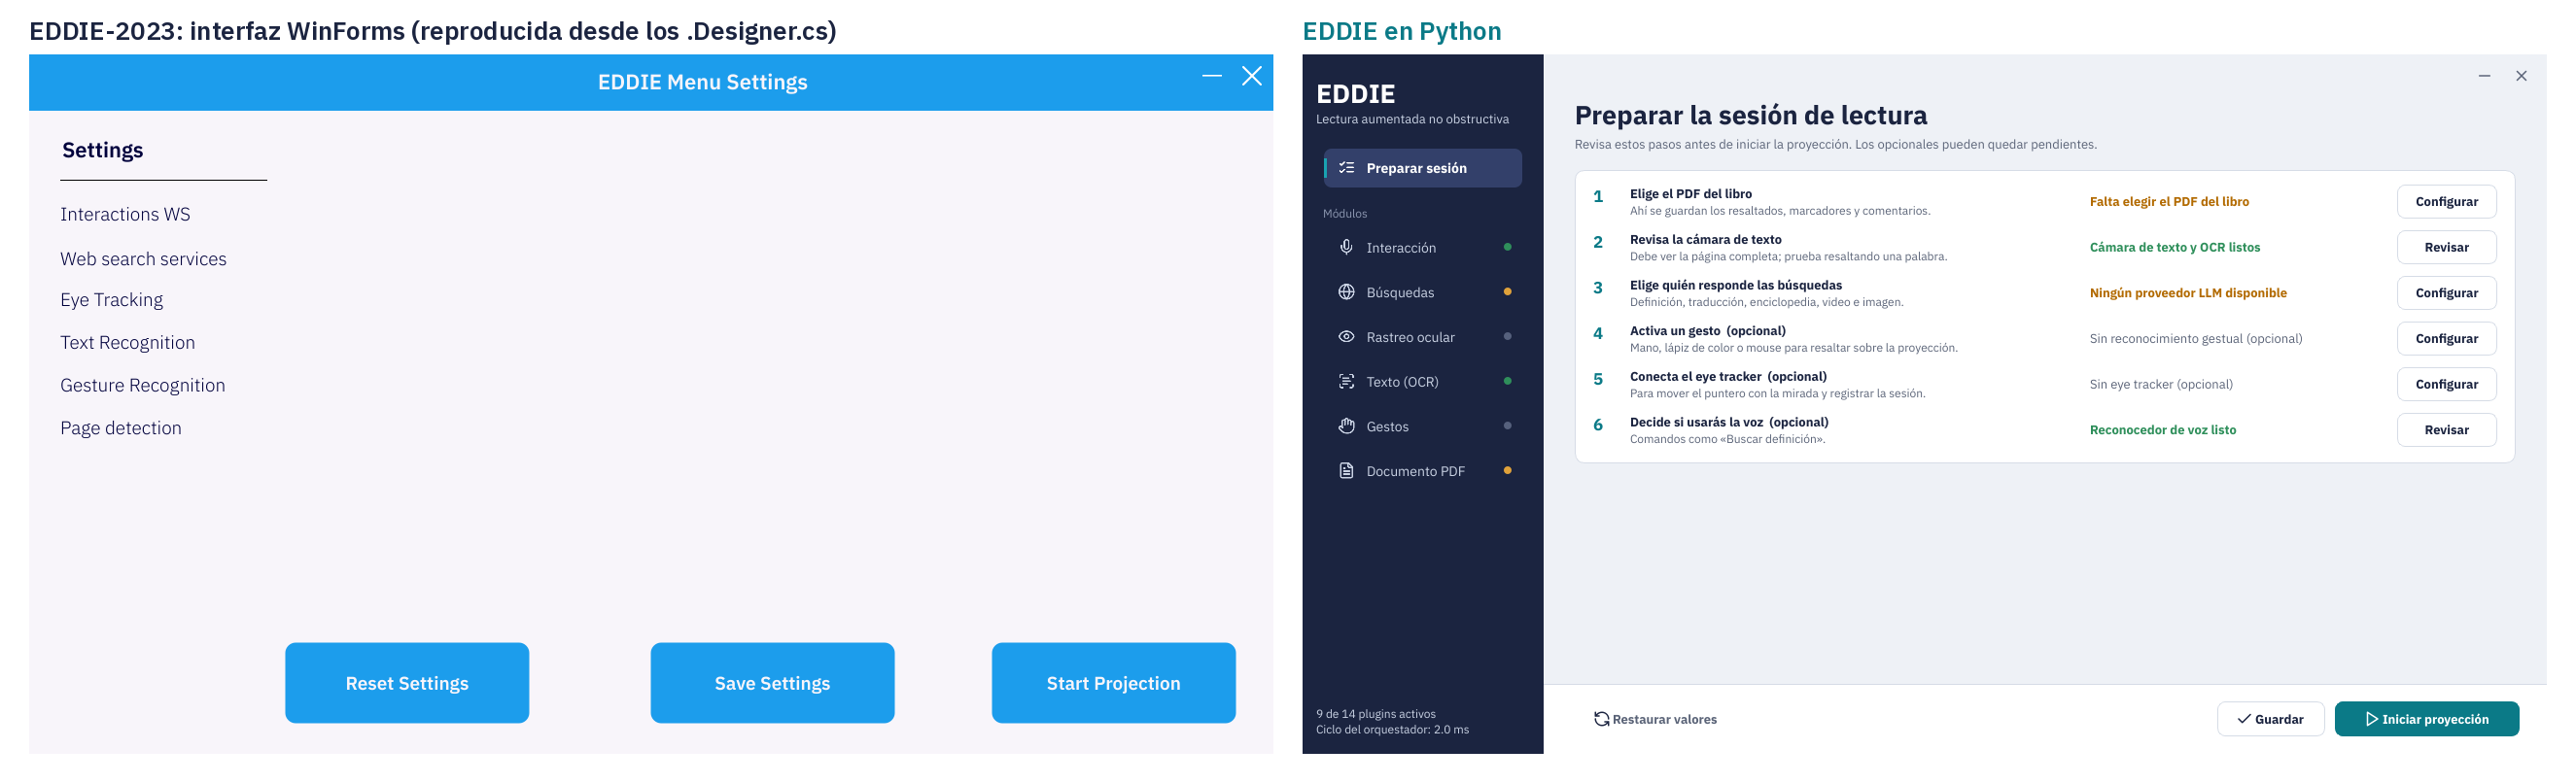
\includegraphics[width=\textwidth]{figuras/comparacion_inicio.png}
\caption{Pantalla de inicio: EDDIE-2023 (izquierda) y versión en Python (derecha).}
\fuente{Elaboración propia.}
\end{figure}

\begin{figure}[H]
\centering
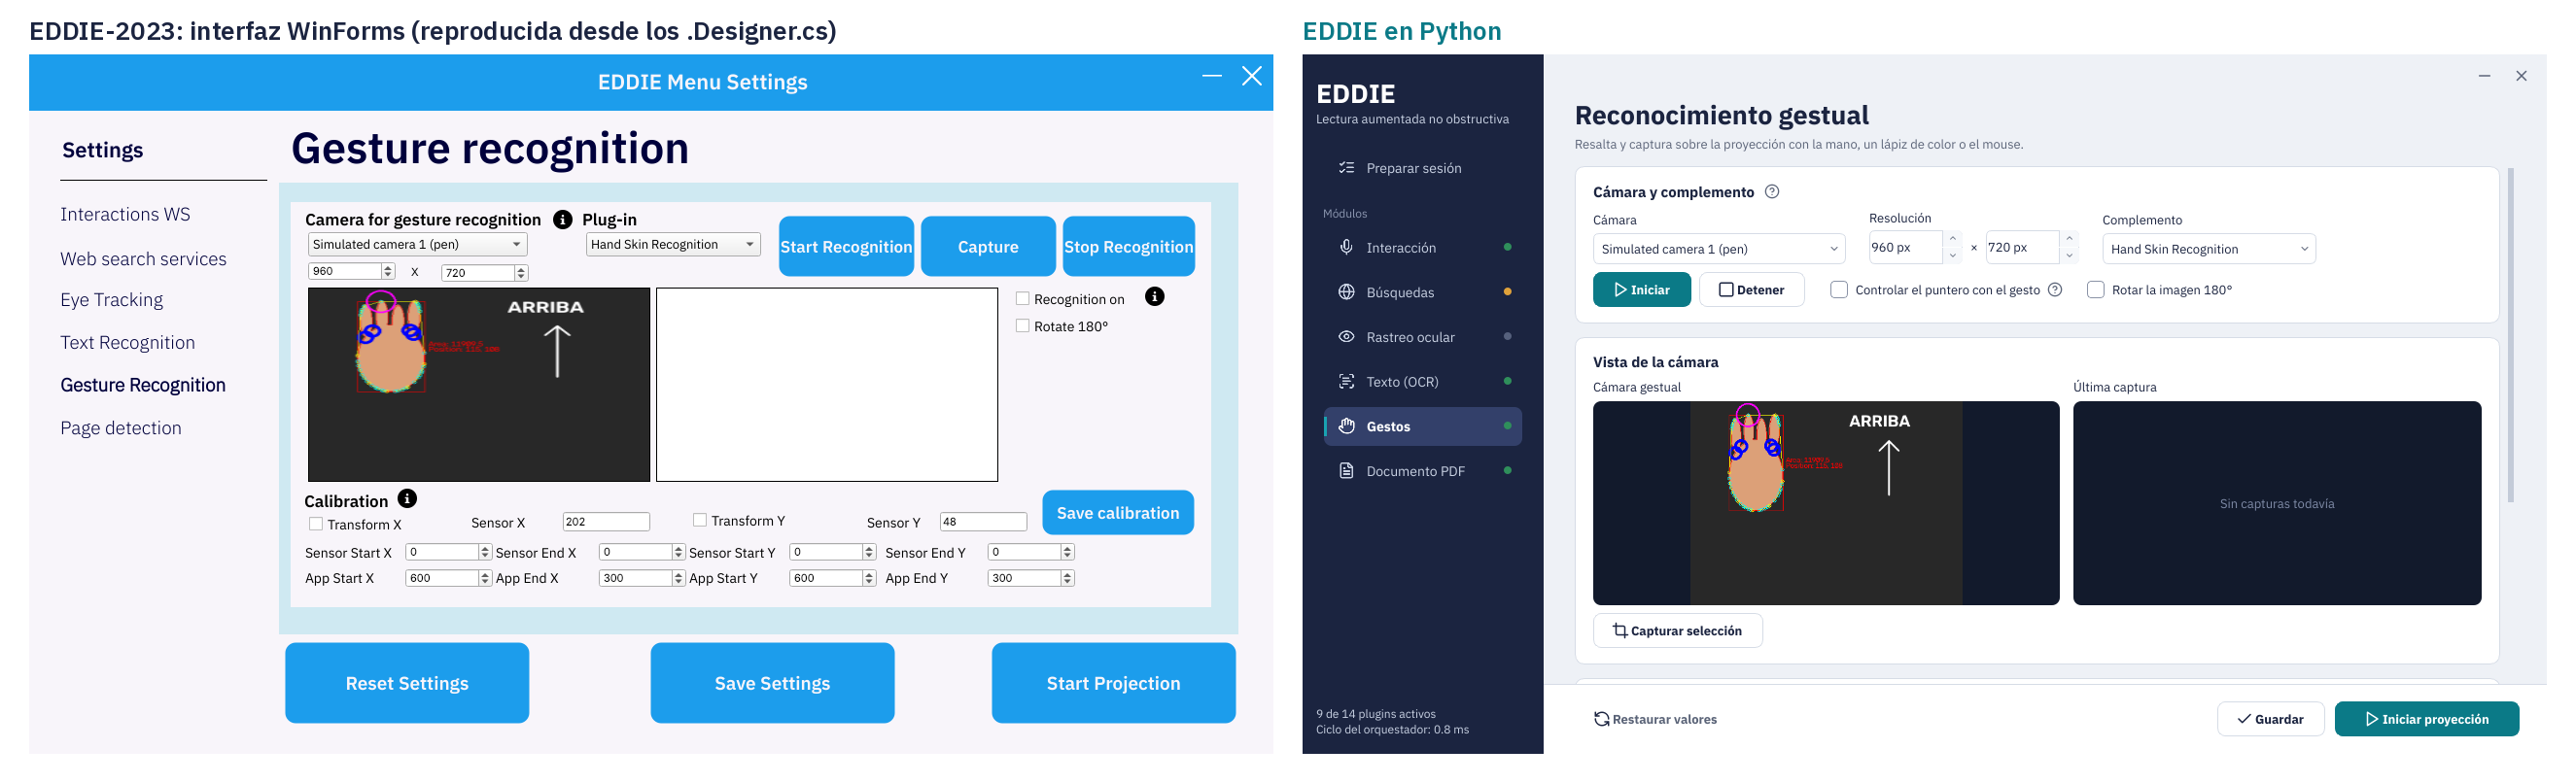
\includegraphics[width=\textwidth]{figuras/comparacion_gestos.png}
\caption{Configuración de gestos: EDDIE-2023 (izquierda) y versión en Python (derecha).}
\fuente{Elaboración propia.}
\end{figure}

\begin{figure}[H]
\centering
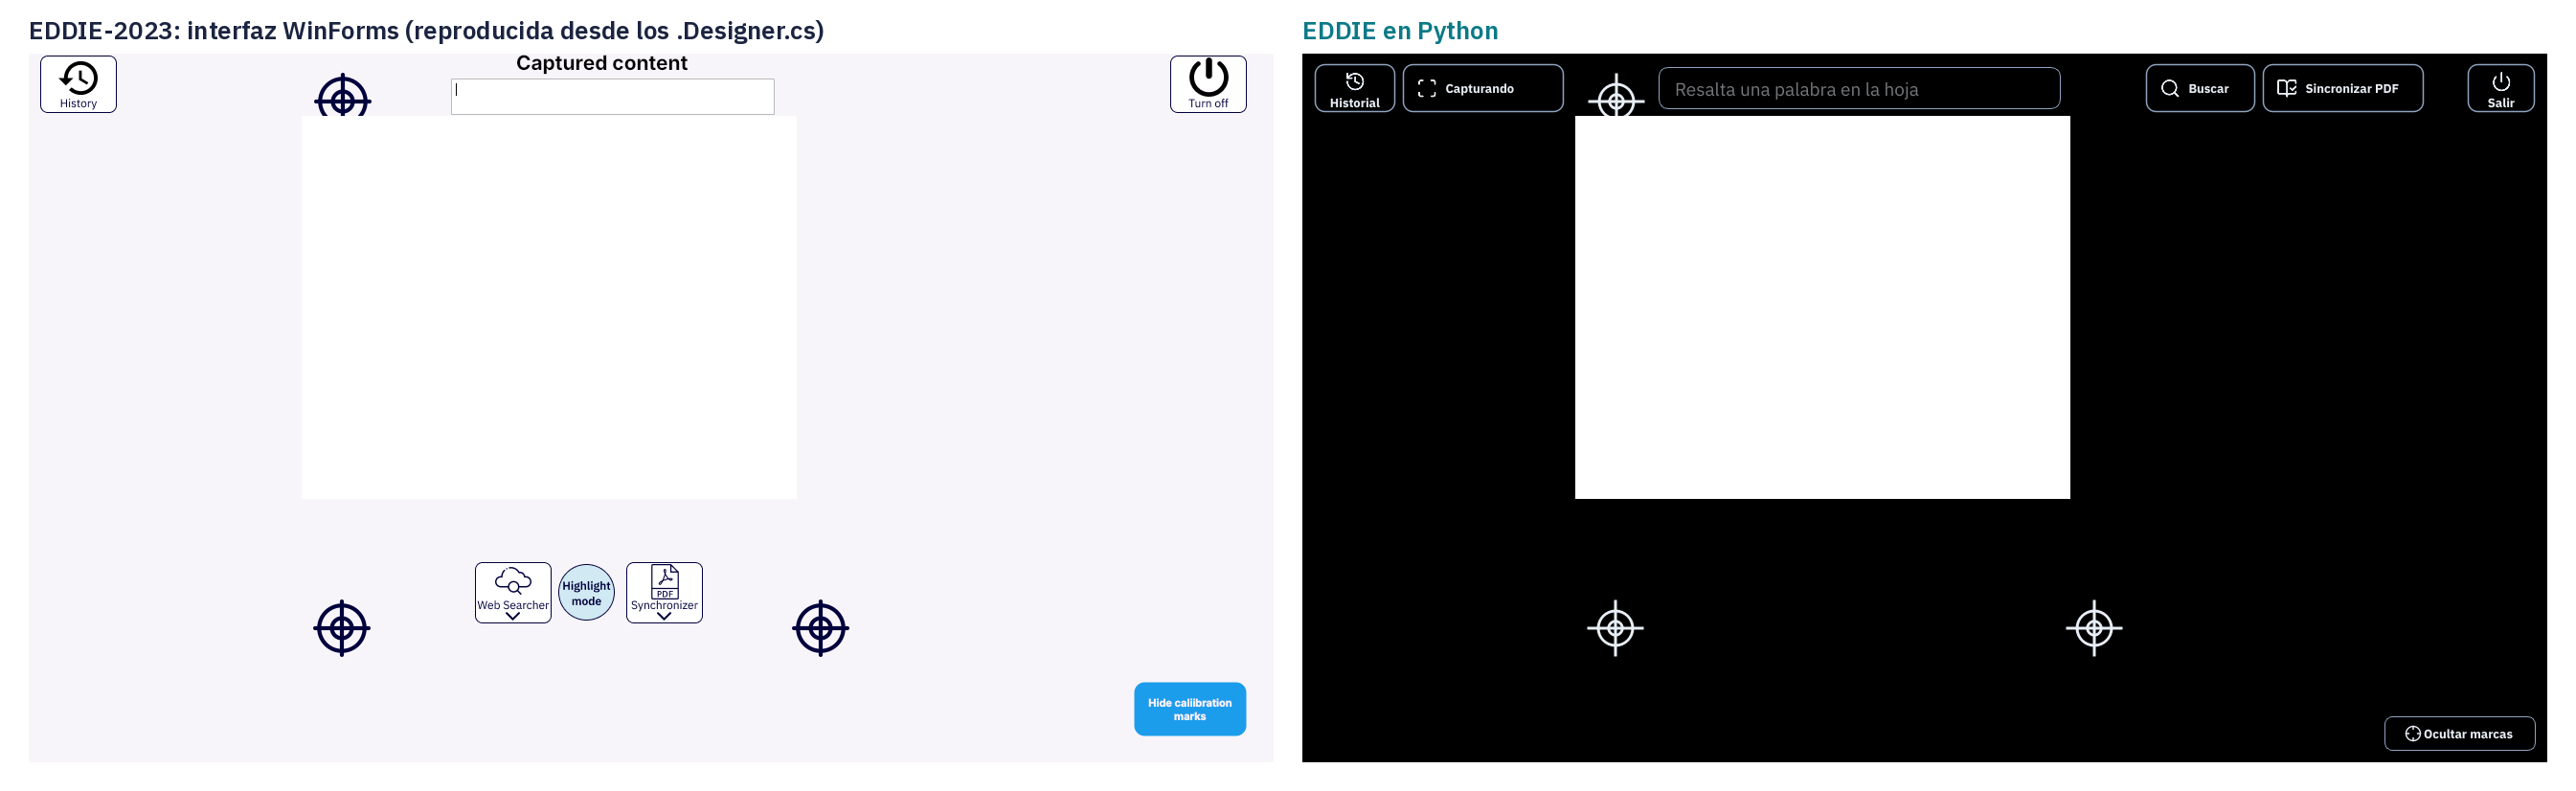
\includegraphics[width=\textwidth]{figuras/comparacion_proyeccion.png}
\caption{Pantalla proyectada: EDDIE-2023 (izquierda) y versión en Python (derecha).}
\fuente{Elaboración propia.}
\end{figure}

\chapter{Manual de instalación y uso}
\label{ap:manual}

\section{Instalación}

\begin{enumerate}
  \item Instalar Python 3.12 (64 bits) y, para el reconocimiento de texto, Tesseract-OCR con el idioma español.
  \item En la carpeta del proyecto:
\begin{verbatim}
python -m venv .venv
.venv\Scripts\activate
pip install -r requirements.txt
\end{verbatim}
  \item Para las búsquedas, copiar \nolinkurl{config/secrets.example.json} como \nolinkurl{config/secrets.json} y pegar la clave de Google AI Studio, o definir la variable \texttt{GEMINI\_API\_KEY}. Este archivo no se sube al repositorio.
  \item Para el rastreo ocular, abrir GazePoint Control o EyeTribe Server antes de conectar el eye tracker desde la aplicación.
\end{enumerate}

\section{Ejecución}

\begin{verbatim}
python main.py              # con el hardware del laboratorio
python main.py --sim        # con cámaras y eye tracker simulados
python -m pytest            # pruebas automatizadas
python tools\generar_evidencias.py   # evidencias
\end{verbatim}

\section{Uso}

\begin{enumerate}
  \item Al abrir, la pantalla de inicio muestra los pasos para preparar la sesión y el estado de cada módulo; cada paso lleva a su página.
  \item En \textit{Texto} y \textit{Gestos}, elegir la cámara y la resolución. En gestos, elegir el complemento (lápiz, mano o mouse), iniciarlo y calibrar apuntando a la cruz superior izquierda y luego a la inferior derecha.
  \item En \textit{Documento PDF}, elegir el PDF del libro.
  \item En \textit{Rastreo ocular}, elegir el eye tracker, la retícula y el registro CSV, y pulsar \textit{Aplicar y conectar}.
  \item Guardar e iniciar la proyección. En la proyección, resaltar una palabra; el texto reconocido aparece en el campo superior y los botones de búsqueda entregan definición, traducción, enciclopedia, video o imagen. \textit{Sincronizar PDF} abre las herramientas de consistencia papel--PDF.
\end{enumerate}

Los ajustes se guardan en \texttt{config/user\_settings.json}, las búsquedas en \texttt{CSV\_registro\_actividades/} y cada acción del orquestador con su latencia en \texttt{logs/}.

\end{document}
